
% ==============================
% Vorspann des LaTeX Dokumentes
% ==============================

% --- Definition der Dokumentenklasse: \documentclass[Optionen]{Klassenname}
% --- Dokumentenklasse gibt zahlreiche Vereinbarungen ueber Layout und Gliederung vor
% --- Wir verwenden hier die KOMA-Script Klasse 'srcreprt'
% --- Siehe dazu Anleitung zum KOMA-Script, insb. Abschnitt 2.6, Kapitel 3,
\documentclass[%
	a4paper,%							Papiergroesse im DIN A4-Format
	oneside,%							Einseitiger Druck
%	twoside,%							Zweiseitiger Druck
	12pt,%								Schriftgroesse
%	draft,%								Option unterscheidet zw. Dokument im Entwurfsstadium und fertigen Dokument
	toc=listof,%					Abbildungs- und Tabellenverzeichnis erhalten einen Eintrag im Inhaltsverzeichnis ohne Nummerierung
	toc=bibliography,%		Literaturverzeichnis erhaelt einen Eintrag im Inhaltsverzeichnis ohne Nummerierung
%	toc=flat,%						Inhaltsverzeichnis erhaelt eine tabellarische Form (ohne Einruecken der unteren Ebenen)
%	chapterprefix,%				Kapitelueberschriften werden nicht in kompakter Form dargestellt
%	appendixprefix%				Anhangueberschriften werden nicht in kompakter Form dargestellt
%	titlepage%						Titel und Zusammenfassung erscheinen auf einer eigenen Seite (Voreinstellung f�r 'book' und 'report')
	fleqn%								Mathematische Formeln werden linksbuendig statt zentriert gesetzt
%	leqno%								Mathematische Formeln werden auf der linken Seite statt auf der rechten Seite nummeriert
]{scrreprt}%


% --- Eigene Stildatei (Hier werden alle grundlegenden Einstellungen fuer Layout und Packages vorgenommen)
% --- Moeglicher Inhalt: Einbindung von haeufig verwendeten Pakete und Erweiterungspaketen
% ---										 Definition eigener Befehle
% ---                    Ausfuehrung global wirkender Befehle (z.B. globale Layout Einstellungen etc.)
\usepackage{styles/abschlussarbeit}


% =============================
%	Hauptdokument mit Textinhalt
% =============================

% --- Aufteilung in mehrere Quelldateien
%			LaTeX unterstuetzt die Aufsplittung in Teildokumente, so dass in einem Uebersetzungslauf nur ein gewisser Anteil verarbeitet wird
%			\include{Dateiname} - bindet 'Dateiname' (ohne .tex Endung) in das Dokument, LaTeX sorgt fuer Seitenumbruch vor und nach dem Inhalt dieser Datei und verwaltet eine eigene Hilfsdatei ('Dateiname'.aux) mit Querreferenzen u.ae.
%			\includeonly{Dateiname,Dateiname,...} - werden nur diejenigen Dateien tatsaechlich mit \include eingebunden, die hier aufgaehlt werden. Ist \includeonly nicht vorhanden, so werden alle Dateien eingebunden.

%\includeonly{chapters/heranfuehrende_kapitel,chapters/hauptteil}

\begin{document}

% --- Titelblatt
% ===========
% Titelseite
% ===========

% --- Kopf- und Fusszeilen der Titelseite sind leer
\thispagestyle{empty}

%\hspace*{1em}
\vfill
	\begin{center}
			\includegraphics[width=10cm]{images/WWU_Logo1_1c}
		\par
		\vspace*{8ex}
\Huge
%			Titel der Abschlussarbeit
			\textsc{L�sung eines Phasenfeld Modells f�r Rissentstehung mittels semiglatter Newtonmethode}
		\par
\normalsize
		\vspace*{8ex}
\large
			\textsc{Bachelorarbeit}\\
%			\textsc{Masterarbeit}\\
%			\textsc{Diplomarbeit}\\
\normalsize
			zur Erlangung des akademischen Grades\\
\large
			\textsc{Bachelor of Science}
%			\textsc{Master of Science}
%			\textsc{Diplom-Mathematiker/in}
		\par
\normalsize
		\vspace*{6ex}
			Westf�lische Wilhelms-Universit�t M�nster\\
			Fachbereich Mathematik und Informatik\\
			Institut f�r Numerische und Angewandte Mathematik
	\end{center}
	\par
	\vspace*{12ex}
	\begin{tabular}{ll}
		Betreuung: \hspace{35ex} & Eingereicht von: \\
		\large
			\textit{Prof. Dr. Benedikt Wirth} &\textit{Ines Ahrens} \\ 
	\end{tabular}
	\par
\normalsize
	\vspace*{4ex}
		M�nster, September 2015
\vfill

% kleine roemische Seitenzahlen im Vorspann der Arbeit, Seitenzaehler wird automatisch auf 1 gesetzt
\pagenumbering{roman}

% --- Zusammenfassung (Abstract)
%
\chapter{Numerische Resultate}

Zuerst betrachten wir die Implementierung der Optimierung. Wir werden darauf eingehen, wie man die Parameter im Code \ref{sec:code} w�hlen muss. Danach werde ich einige Beispiele f�r unterschiedliche Gitterweiten, verschiedene Risse und M�glichkeiten des Einspannens des Materials betrachten.   

\section{Justieren der Parameter im Code}

Am Anfang ist zu sagen, dass wir nur Risse betrachten, die mindestens zwei Gitterpunkte breit sind. Wenn ein Riss nur einen Gitterpunkt breit ist, wird $v$ nicht konstant $0$, was dazu f�hrt, dass in der Implementation nie ein vollst�ndiger Riss vorhanden ist.   

Au�erdem muss $u_0$ an beiden R�ndern unterschiedlich sein. Wenn $u_0$ an beiden R�ndern gleich ist, ist die Verschiebung des Materials �berall gleich, d.h. dass nur eine Translation stattgefunden hat. Selbst wenn wir einen Riss einf�gen, werden wir diesen nicht sehen. 

%Als erstes treffen wir eine Wahl f�r $\epsilon_1$ und $\epsilon_2$. F�r $\epsilon_1$ muss gelten: $\epsilon_1<\frac{1}{k}$, wobei $k$ die Anzahl der Gitterpunkte ist. 
%%todo warum?  
%F�r $\epsilon_2$ muss gelten: $\epsilon_2>\frac{1}{k}$, 
%%todo warum? da epsilon die breite des Risses darstellt??? ca 

Zur Wahl von der Konstanten $c$, die durch den Lagrangemultiplikator $\eta$ hinzugekommen ist: W�hlt man $c$ zu gro� und betrachtet
\begin{align*}
	f(v,\eta)=  \eta - \max\{0, \eta + c(v-v_0)\}- \min\{0, \eta + c v\}				
\end{align*}
werden das Maximum und das Minimum 0, da $v-v_0$ negativ ist und $v$ positiv ist. Es gilt $f(v,\eta)= \eta$. Nach dem Newtonverfahren ist $-G_2 = \partial G_{2v} s_1^k + \partial G_{2 \eta} s_2^k$ mit 
\begin{align*}
	G_2 = (\int\limits_{\Omega} T_i T_j \diff_x)_{ij}  \eta^h \hspace{9ex}
	\partial G_{2v}  = 0 \hspace{9ex}
	\partial G_{2 \eta}  = (\int\limits_{\Omega} T_i T_j \diff x)_{ij} 
\end{align*} 
Daraus folgt $\eta^h = - s^k$. Au�erdem gilt $\eta^{k+1}= \eta^k + s^k= 0$. Dadurch fallen nach dem ersten Iterationsschritt alle Terme mit $\eta$ weg. Also ber�cksichtigen wir die vorgegebene Bedingung von $0<v<v_0$ nicht mehr. Diese soll aber explizit ber�cksichtigt werden. Also sollte man $c$ nicht zu gro� w�hlen. Auch wenn $c$ zu klein gew�hlt wird, beachten wir die Schranke nicht, d.h. sinnvollerweise sollte man ungef�hr $c=1$ w�hlen. 

Die richtige Wahl von $\eta$ am Anfang zu finden, ist gar nicht so einfach. $\eta$ kann positiv und negativ sein, da $\eta=\lambda - \mu$ ist, wobei $\lambda>0, \mu>0$ Lagrangemultiplikatoren sind. Experimentell findet man heraus, dass $\eta=1$ kein Ergebnis liefert, bei $\eta \ge 2$ fast kein �bergang zwischen Riss und nicht Riss ist, bei $0,4<\eta<1$ ist das Papier nicht richtig gerissen, also $v$ wird nie ganz 0 und/oder das Papier ist nie ganz heile, d.h. 1 wird nie angenommen. Die Wahl von $\eta=0,34$ ist f�r manche Probleme sehr gut, f�r andere nicht. Erst im negativen Bereich erhalten wir f�r alle Probleme gute Werte. Hier muss aber  $\eta >-1 $ gelten. 
%todo f�r wahl eta grafiken einf�gen?

Kommen wir zur Wahl von $v_0$. Es sollte Sinn ergeben, $v_0$ konstant in einer Umgebung von 1 zu w�hlen, da $v=1$ schon bedeutet, dass kein Riss vorhanden ist. Kleiner sollte es nicht gew�hlt werden, da sonst nicht zugelassen ist, dass das Gebiet nicht gerissen ist. Dies ist leider in der Implementation nicht zu sehen. Bei $v_0>0,7$ erhalten wir Ergebnisse, die mit den erwarteten Ergebnissen �bereinstimmen. Damit ist auch  $v>v_0$, was im Widerspruch zu der Nebenbedingung $0<v<v_0$ steht.  Au�erdem ver�ndern auch gro�e Werte von $v_0$ nichts am Ergebnis. Dieses Verhalten l�sst �berlegen, ob es �berhaupt sinnvoll ist, diese Bedingung mit in das Problem zu nehmen. Als weiteren Ansatz k�nnte die Rissentstehung auch ohne Ungleichungsnebenbedingungen getestet werden. 

\section{Beispiele}
Mit dem implementierten Algorithmus k�nnen wir nun einige Beispiele betrachten. Dazu betrachten wir zwei unterschiedliche Grafiken, z.B. \ref{fig:riss_ganz_mitte.riss} und \ref{fig:riss_ganz_mitte.gebiet}. In einer Grafik ist die Verschiebung des Gebietes dargestellt, in der anderen, ob und wie stark ein Riss vorhanden ist. Bei beiden Grafiken ist jeweils das gesamte Gebiet, hier ein rechteckiges Gebiet in 2D auf der x und y Koordinate dargestellt. Die z Koordinate gibt bei der Verschiebung an, wie stark das Gebiet verschoben ist und bei dem Riss, wie stark der jeweilige Gitterpunkt eingerissen ist. Ein Wert in der N�he von 1 bedeutet, dass das Gebiet nicht gerissen ist und 0, dass es vollst�ndig gerissen ist. 

Bei beiden Grafiken sind je 8 Bilder zu sehen. Diese geben an, wie viele Iterationsschritte der Newton Algorithmus durchgelaufen ist. Das erste Bild (also links oben) gibt das Ergebnis nach der ersten Iteration an. Das zweite Bild, rechts neben dem ersten Bild, gibt das Ergebnis nach 2 Schritten aus. Dann folgen 5, 10, 20, 50, 100 und zum Schluss, rechts unten, 200 Iterationsschritte. 

\subsection{Der Riss im Material ist durchg�ngig}

Beim ersten Beispiel ist das Gebiet an der rechten und linken Seite konstant eingespannt. Hier ist $u$ am linken Rand immer 1 und am rechten Rand immer 2. Am Anfang wurde ein Riss durch das gesamte Gebiet eingef�gt, der parallel zum eingespannten Rand verl�uft. Dieser befindet sich genau in der Mitte des Gebietes. Dieses sieht man auch in dem ersten Bild von \ref{fig:riss_ganz_mitte.riss}.

Betrachtet man den Riss im Verlauf der Iterationen, sieht man, dass der Riss an der gleichen Stelle bleibt und gegl�ttet wird. Manchmal schwankt das Gebiet, das nicht gerissen ist, zwischen $0,9$ und $1,1$.  
Die Verschiebung des Gebietes  \ref{fig:riss_ganz_mitte.gebiet}  sieht �hnlich aus. An der Stelle des Risses, ist eine Unstetigkeitsstelle zu finden. Diese zieht sich durch alle Bilder. Die Ver�nderung im Verlauf der Iterationen ist zum einen, dass die Unstetigkeit gegl�ttet wird. Zum anderen ist die Verschiebung, die nicht beim Riss ist, linear und mit steigender Iterationszahl fast konstant.  

Die Gl�ttung des Risses, und damit auch die Gl�ttung der Unstetigkeitsstelle bei der Verschiebung im Gebiet, entsteht durch den $|\nabla v|^2$ Term im Optimierungsproblem, wie am Anfang erl�utert. Ebenfalls ist die zun�chst lineare und dann ann�hernd konstante Verschiebung hierauf zur�ckzuf�hren.
Der Riss breitet sich nicht weiter aus, da das Gebiet nicht weiter verschoben wird. Dieses Szenario liefert realit�tsnahe Ergebnisse. 

Betrachten wir das gleiche Szenario bei einem $10 \times 10$ Gitter wie in \ref{fig:riss_ganz_mitte_10_gitter.gebiet} und \ref{fig:riss_ganz_mitte_10_gitter.riss}. Hier gibt es andere Ergebnisse. Der Riss verschiebt sich zum Rand, an dem $v=1$ gilt. Vermutlich liegt die Verschiebung des Risses daran, dass der Riss sehr gro� im Vergleich zu dem Gitter ist. Dadurch wird das gesamte Papier gerissen, was niedriger eingespannt ist. 

\newpage 
\begin{figure}[!htb]
	\centering 
	\includegraphics[scale=0.429]{images/optimazation/01rissGanz_Gitter_100_u0Konstant.png}
	\caption{Darstellung der Verschiebung des Gebietes bei konstantem $u_0$, einem Riss in der Mitte und $100\times 100$ Gitterpunkten}
	\label{fig:riss_ganz_mitte.gebiet}
\end{figure}

\begin{figure}[!htb]
	\centering	\includegraphics[scale=0.429]{images/optimazation/02rissGanz_Gitter_100_u0Konstant.png}
	\caption{Darstellung des Risses  bei konstantem $u_0$, einem Riss in der Mitte und $100\times 100$ Gitterpunkten}
	\label{fig:riss_ganz_mitte.riss}
\end{figure}

\newpage

\begin{figure}[!htb]
	\centering 
	\includegraphics[scale=0.8]{images/optimazation/01rissGanz_Gitter10_u0Konstant.png}
	\caption{Darstellung der Verschiebung des Gebietes  bei konstantem $u_0$, einem Riss in der Mitte und $10\times 10$ Gitterpunkten}
	\label{fig:riss_ganz_mitte_10_gitter.gebiet}
\end{figure}

\begin{figure}[!htb]
	\centering	\includegraphics[scale=0.8]{images/optimazation/02rissGanz_Gitter10_u0Konstant.png}
	\caption{Darstellung des Risses  bei konstantem $u_0$, einem Riss in der Mitte und $10\times 10$ Gitterpunkten}
	\label{fig:riss_ganz_mitte_10_gitter.riss}
\end{figure}

\newpage



\subsection{Das Material ist am Rand angerissen}

Beim n�chsten Experiment betrachten wir das gleiche $u$ wie vorhin, aber wir rei�en das Papier nur an einer Seite ein wenig an. Dieser Riss ist 10 Gitterpunkte lang auf einem $100 \times 100$ Gitter. Abbildung \ref{fig:riss_klein_100_gitter.gebiet} und \ref{fig:riss_klein_100_gitter.riss} zeigen dieses Szenario. 

Betrachten wir zun�chst die Verschiebung des Gebietes. Hier sieht man nur dort eine Unstetigkeitsstelle, wo am Anfang der Riss ist. Diese Unstetigkeitsstelle wird l�nger und breitet sich parallel zur Befestigung aus. Am Ende, bei 200 Iterationen, ist im gesamten Papier der Riss zu sehen. Die Unstetigkeitsstelle wird wieder glatter, je mehr Iterationen das Programm durchgef�hrt hat.     

Auch die Ausbreitung des Risses verl�uft fast identisch. W�hrend der ersten 20 Iterationen ist kaum eine Ver�nderung festzustellen. Bei der 50. Iteration liegt der Wert von v bei 0,7 dort, wo das Extremum nicht angenommen wird. Bei sp�teren Iterationen zieht sich der Riss wie erwartet durch die gesamte Oberfl�che.
  
Im Groben zeigt der Algorithmus das erwartete Verhalten, d.h. der Riss breitet sich parallel zur Befestigung aus. Die Anomalie bei Iteration 50 k�nnte eine Ungenauigkeit in meinem Algorithmus oder der zu Grunde liegenden Modellierung sein. 

\newpage 

\begin{figure}[!htb]
	\centering	\includegraphics[scale=0.91]{images/optimazation/01riss1Rand_Gitter_100_u0Konstant.png}
	\caption{Verschiebung des Gebietes bei konstantem $u_0$, einem kleinen Riss am Rand und $100\times 100$ Gitterpunkten}
	\label{fig:riss_klein_100_gitter.gebiet}
\end{figure}

\begin{figure}[!htb]
	\centering	\includegraphics[scale=0.42]{images/optimazation/02riss1Rand_Gitter_100_u0Konstant.png}
	\caption{Darstellung des Risses  bei konstantem $u_0$, einem kleinen Riss am Rand und $100\times 100$ Gitterpunkten}
	\label{fig:riss_klein_100_gitter.riss}
\end{figure}

\newpage 

\subsection{Das Material ist an beiden Seiten eingerissen}


Befestigen wir nun das Material wieder wie vorhin und rei�en es an beiden Seiten an, sodass die Risse aufeinander zulaufen. Dies stellen Abbildung \ref{fig:riss_aufeinanderzulaufend_100_gitter.gebiet} und \ref{fig:riss_aufeinanderzulaufend_100_gitter.riss} dar. 

Zun�chst wird der Riss bei beiden Bildern nur gegl�ttet. Sp�ter setzt er sich fort, sodass beide Risse zu einem Riss werden. Dadurch erh�lt man einen Riss, der quer durch das gesamte Material verl�uft. 

Dieses ist auch das erwartete Verhalten des Risses. 

\begin{figure}[!htb]
	\centering	\includegraphics[scale=0.24]{images/optimazation/01Riss2gegeneinanderausgerichtet_Gitter_100_u0_konstant.png}
	\caption{Verschiebung des Gebietes bei konstantem $u_0$, einem kleinen Riss an beiden R�ndern und $100\times 100$ Gitterpunkten}
	\label{fig:riss_aufeinanderzulaufend_100_gitter.gebiet}
\end{figure}

\begin{figure}[!htb]
	\centering	\includegraphics[scale=0.35]{images/optimazation/02Riss2gegeneinanderausgerichtet_Gitter_100_u0_konstant.png}
	\caption{Darstellung des Risses  bei konstantem $u_0$, einem kleinen Riss an beiden R�ndern und $100\times 100$ Gitterpunkten}
	\label{fig:riss_aufeinanderzulaufend_100_gitter.riss}
\end{figure}

%Kommen wir zu einem Beispiel, wo das Programm nicht das erwartete tut.

%\subsection{Das Material ist an einer Seite an zwei Stellen eingerissen}
%
%\begin{figure}[ht]
%	\centering	\includegraphics[scale=0.3]{images/optimazation/01_2_rissAnEinerSeite_100Gitter_u0Konstant.png}
%	\caption{Darstellung des Risses bei konstantem $u_0$, einem kleinen Riss an beiden R�ndern und $100x100$ Gitterpunkten}
%	\label{fig:2riss_eineSeite_100_gitter.gebiet}
%\end{figure}
%
%\begin{figure}[ht]
%	\centering	\includegraphics[scale=0.42]{images/optimazation/02_2_rissAnEinerSeite_100Gitter_u0Konstant.png}
%	\caption{Darstellung des Risses  bei konstantem $u_0$, einem kleinen Riss an beiden R�ndern und $100x100$ Gitterpunkten}
%	\label{fig:2riss_eineSeite_100_gitter.riss}
%\end{figure}
%
%Die Befestigung des Materials ist wieder dieselbe wie vorhin. Nun rei�en wir das Papier an einer Seite so ein, dass sich die Risse 


% --- Inhaltsverzeichnis wird automatisch erzeugt
\tableofcontents

% technische Gruende, damit Inhaltsverzeichnis roemische Seitenzahl erhaelt
\newpage
% arabische Seitenzahlen im Rest der Arbeit, Seitenzaehler wird automatisch auf 1 gesetzt
\pagenumbering{arabic}

% --- Einleitung (Introduction)
%% ====================================
% Einleitung
% ====================================

\chapter{Einleitung}
\label{chap:einleitung}

%todo Konvergenz S 38 in Script 
%englischer Titel: solution of a phase field model for crack formation using semismooth newton methods

%todo anderer Anfangssatz
Wir wollen herausfinden, wie Risse entstehen, bzw wie sie sich fortsetzen,

%\begin{itemize}
%	\item Was beschreibt mein Problem? Warum minimiere ich da?
%	\item Was besagen die einzelnen Terme? fertig
%	\item Was mache ich in meiner Bachelorarbeit damit/ wie mache ich es
%\end{itemize}
%todo was ist ein phasenfeld?
%todo referenzen einf�gen!
Betrachten wir zun�chst ein Beispiel. Ein Blatt Papier befindet sich in Ruheposition auf dem Gebiet $\Omega \subset \R^3 $.Nun wird es an zwei gegen�berliegenden Seiten eingespannt und an diesen Seiten wird Kraft ausge�bt. Was passiert? Zun�chst wird sich das Blatt Papier ein wenig dehnen, also deformieren. Die neue Position des Papiers beschreibt $\varphi(x)$. Also gilt $\varphi=u+id$ wobei $u$ die Verschiebung des K�rpers ist. 

Das Ziel ist es, obwohl Kraft auf dem K�rper ausge�bt wird, dass die Verzerrung des Papiers minimal ist. Dazu betrachten wir den Abstand zwischen $x \in \Omega$ und $ x+h \in \Omega$ im aktuellen Zustand
\begin{align*}
	\|\varphi(x+h)- \varphi(x)\|^2 = \|\nabla \varphi \|^2 + o(\|h\|^2) = h^T \nabla \varphi^T \nabla \varphi h + o(\|h\|^2)
\end{align*} 
Damit haben wir die Matrix $C:=\nabla \varphi^T \nabla \varphi $ erhalten, die die lokale �nderung der L�ngen angibt. Diese nennt sich Cauchy-Grennscher Verzerrungstensor. 
Die Verzerrung $E$ ist $ \frac{1}{2} (C-I)$. Da $u=\phi - \text{id}$ gilt, k�nnen wir die Ableitung von u einsetzen und erhalten
\begin{align*}
	E_{ij}=\frac{1}{2} \left( \frac{\partial  u_i}{\partial x_j} +\frac{\partial  u_j}{\partial x_i}  \right) + \frac{1}{2} \sum\limits_{k} \frac{\partial  u_i}{\partial x_k} \frac{\partial  u_j}{\partial x_k} 
\end{align*}
Da im linearen die quadratischen Terme vernachl�ssigt werden k�nnen, erhalten wir $ \frac{1}{2} \left( \frac{\partial  u_i}{\partial x_j} +\frac{\partial  u_j}{\partial x_i} \right) = \frac{\nabla u^T + \nabla u}{2} $.

Wenn kr�ftiger am Papier gezogen wird, rei�t es. Dann ist die Formel f�r die Verzerrung nicht mehr g�ltig. Also brauchen wir einen Term, der angibt, wo und wie stark der K�rper gerissen ist.  $v: \Omega \rightarrow \R$ ist 0, falls der K�rper vollst�ndig gerissen ist und 1, wenn kein Riss vorhanden ist.  Multiplizieren wir also $ \frac{1}{2} (\nabla u^T + \nabla u)$ mit  $v^2 + \epsilon_1$. Es ergibt sich 
\begin{align*}
	& \min\limits_u \int\limits_{\Omega} |\nabla u|^2 (v^2 + \epsilon_1) \\
	& u=u_0 \text{ auf } \Gamma_1 \cup \Gamma_2  
\end{align*}
Da wir $u$ nur im zweidimensionalen betrachten, k�nnen wir  $\frac{\nabla u + \nabla u^T}{2}^2$ vereinfachen zu $|\nabla u|^2$. Der K�rper ist an $\Gamma_1$ und $\Gamma_2$ befestigt, was die Randbedingung $u_0$ angibt.  

In der Modellierung w�re es nun ideal, falls der K�rper nie rei�t. Dies ist jedoch nicht m�glich. Betrachten wir deswegen den Riss genauer. Einerseits wollen wir, dass der Riss m�glichst klein ist, also die Oberfl�che, auf der der Riss auftritt m�glichst minimal ist. Anderersetits stellen wir fest, dass, wenn ein Riss vorhanden ist, immer ein �bergang zwischen dem Riss und dort wo es nicht gerissen ist, ist. 
Betrachten wir zun�chst die Minimierung der Oberfl�che. Wir wollen also, dass $\int\limits_{\Omega} (1-v)^2$ minimal ist. Aber in der Realit�t stellt man fes, dass es Zwischenst�ck zwischen Riss un nicht Riss gibt. Damit dieses gen�gend glatt ist, addieren wir die Ableitung zum Quadrat mit $\epsilon_2^2$ multipliziert hinzu. Daraus ergibt sich eine Darstellung vom Riss
\begin{align*}
	\epsilon_2 |\nabla v|^2 + \frac{1}{\epsilon_2} (1-v)^2
\end{align*}
Zusammengefasst ist das gesamte Problem gegeben durch
\begin{align*}
	& \min\limits_{u \in  \h^2 , v \in \h } \int_{\Omega} \left( v^2 + \epsilon_1 \right) | \nabla u|^2 + \nu \left(\epsilon_2 |\nabla v|^2 + \frac{1}{\epsilon_2} \left( 1- v \right)^2 \right) dx \\
	& \text{s.d.} \hspace{1ex} 0 \le v \le v_0 \\\
	& u=u_0 \text{ auf } \Gamma_1 \cup \Gamma_2  
\end{align*}
dabei ist $\nu$ eine Konstante, $\epsilon_i>0 \hspace{1ex}\forall i \in \{1,2\}$ ein kleiner Parameter und $\Gamma_1, \Gamma_2 \subset \Omega$  der rechte bzw. linke Rand eines rechteckigen Gebietes $\Omega \subset \R^2$, d.h., $\Omega=[0,a] \times [0,b] \hspace{1ex} \Gamma_1=\{0\} \times [0,b] \hspace{1ex} \Gamma_2=\{a\} \times [0,b] $
 
$u:\Omega \rightarrow \R^2 $ beschreibt die Verschiebung eines K�rpers auf dem Gebiet $\Omega$. Der K�rper ist an $\Gamma_1$ und $\Gamma_2$ befestigt, was die Randbedingung $u_0$ angibt.  
$v: \Omega \rightarrow \R$ gibt an, wo und wie stark der K�rper gerissen ist. 0 bedeutet, dass der K�rper vollst�ndig gerissen ist und 1, das kein Riss vorhanden ist.    

Zur L�sung des Problems, werden analytische und numerische Grundlagen gebraucht. F�r die analytische Betrachtung nutze ich partielle Differentialgleichungen und Optimierung. Da die L�sung des Problems analytisch nicht zu finden ist, diskretisiere ich das Problem mit dreieckig lineare Lagrange Elemente und implementiere es mittels semiglatter Newton Methoden. Die Grundlagen dazu sind im zweiten Kapitel zu finden. Alle Themen sind sehr umfangreich und ich werde nur die wichtigsten Begriffe einf�hren k�nnen. 
 
Die Untersuchung des Problems folgt in Kapitel drei. Beim ersten Betrachten f�llt auf, dass die Optimierung nach $u$ und $v$ getrennt werden kann. Dieses wird im ersten Teil des dritten Kapitels erl�utert. Im zweiten Teil wird die Optimierung nach $u$ betrachtet. Zuerst wird die Existenz und Eindeutigkeit gesichert, um dann numerisch die L�sung mit dreieckig linearen Lagrange Elementen zu suchen. Die Optimierung nach $v$ im dritten Teil hat den selben Aufbau. Nur ist hier das Problem komplizierter und die numerische L�sung erfolgt mit der semiglatten Newton Methode. 
Im letzten Kapitel werte ich die numerischen Resultate aus und ziehe R�ckschl�sse f�r die Konvergenz der Methode aufgrund der Gitterweite.  
%todo sp�ter �berpr�fen, ob ich das wirklich tue, wenns geschrieben ist



%----- Problemstellung (Problemstellung)
% ====================================
% Einleitung
% ====================================

\chapter{Einleitung}
\label{chap:einleitung}

%todo Konvergenz S 38 in Script 
%englischer Titel: solution of a phase field model for crack formation using semismooth newton methods

%todo anderer Anfangssatz
Wir wollen herausfinden, wie Risse entstehen, bzw wie sie sich fortsetzen,

%\begin{itemize}
%	\item Was beschreibt mein Problem? Warum minimiere ich da?
%	\item Was besagen die einzelnen Terme? fertig
%	\item Was mache ich in meiner Bachelorarbeit damit/ wie mache ich es
%\end{itemize}
%todo was ist ein phasenfeld?
%todo referenzen einf�gen!
Betrachten wir zun�chst ein Beispiel. Ein Blatt Papier befindet sich in Ruheposition auf dem Gebiet $\Omega \subset \R^3 $.Nun wird es an zwei gegen�berliegenden Seiten eingespannt und an diesen Seiten wird Kraft ausge�bt. Was passiert? Zun�chst wird sich das Blatt Papier ein wenig dehnen, also deformieren. Die neue Position des Papiers beschreibt $\varphi(x)$. Also gilt $\varphi=u+id$ wobei $u$ die Verschiebung des K�rpers ist. 

Das Ziel ist es, obwohl Kraft auf dem K�rper ausge�bt wird, dass die Verzerrung des Papiers minimal ist. Dazu betrachten wir den Abstand zwischen $x \in \Omega$ und $ x+h \in \Omega$ im aktuellen Zustand
\begin{align*}
	\|\varphi(x+h)- \varphi(x)\|^2 = \|\nabla \varphi \|^2 + o(\|h\|^2) = h^T \nabla \varphi^T \nabla \varphi h + o(\|h\|^2)
\end{align*} 
Damit haben wir die Matrix $C:=\nabla \varphi^T \nabla \varphi $ erhalten, die die lokale �nderung der L�ngen angibt. Diese nennt sich Cauchy-Grennscher Verzerrungstensor. 
Die Verzerrung $E$ ist $ \frac{1}{2} (C-I)$. Da $u=\phi - \text{id}$ gilt, k�nnen wir die Ableitung von u einsetzen und erhalten
\begin{align*}
	E_{ij}=\frac{1}{2} \left( \frac{\partial  u_i}{\partial x_j} +\frac{\partial  u_j}{\partial x_i}  \right) + \frac{1}{2} \sum\limits_{k} \frac{\partial  u_i}{\partial x_k} \frac{\partial  u_j}{\partial x_k} 
\end{align*}
Da im linearen die quadratischen Terme vernachl�ssigt werden k�nnen, erhalten wir $ \frac{1}{2} \left( \frac{\partial  u_i}{\partial x_j} +\frac{\partial  u_j}{\partial x_i} \right) = \frac{\nabla u^T + \nabla u}{2} $.

Wenn kr�ftiger am Papier gezogen wird, rei�t es. Dann ist die Formel f�r die Verzerrung nicht mehr g�ltig. Also brauchen wir einen Term, der angibt, wo und wie stark der K�rper gerissen ist.  $v: \Omega \rightarrow \R$ ist 0, falls der K�rper vollst�ndig gerissen ist und 1, wenn kein Riss vorhanden ist.  Multiplizieren wir also $ \frac{1}{2} (\nabla u^T + \nabla u)$ mit  $v^2 + \epsilon_1$. Es ergibt sich 
\begin{align*}
	& \min\limits_u \int\limits_{\Omega} |\nabla u|^2 (v^2 + \epsilon_1) \\
	& u=u_0 \text{ auf } \Gamma_1 \cup \Gamma_2  
\end{align*}
Da wir $u$ nur im zweidimensionalen betrachten, k�nnen wir  $\frac{\nabla u + \nabla u^T}{2}^2$ vereinfachen zu $|\nabla u|^2$. Der K�rper ist an $\Gamma_1$ und $\Gamma_2$ befestigt, was die Randbedingung $u_0$ angibt.  

In der Modellierung w�re es nun ideal, falls der K�rper nie rei�t. Dies ist jedoch nicht m�glich. Betrachten wir deswegen den Riss genauer. Einerseits wollen wir, dass der Riss m�glichst klein ist, also die Oberfl�che, auf der der Riss auftritt m�glichst minimal ist. Anderersetits stellen wir fest, dass, wenn ein Riss vorhanden ist, immer ein �bergang zwischen dem Riss und dort wo es nicht gerissen ist, ist. 
Betrachten wir zun�chst die Minimierung der Oberfl�che. Wir wollen also, dass $\int\limits_{\Omega} (1-v)^2$ minimal ist. Aber in der Realit�t stellt man fes, dass es Zwischenst�ck zwischen Riss un nicht Riss gibt. Damit dieses gen�gend glatt ist, addieren wir die Ableitung zum Quadrat mit $\epsilon_2^2$ multipliziert hinzu. Daraus ergibt sich eine Darstellung vom Riss
\begin{align*}
	\epsilon_2 |\nabla v|^2 + \frac{1}{\epsilon_2} (1-v)^2
\end{align*}
Zusammengefasst ist das gesamte Problem gegeben durch
\begin{align*}
	& \min\limits_{u \in  \h^2 , v \in \h } \int_{\Omega} \left( v^2 + \epsilon_1 \right) | \nabla u|^2 + \nu \left(\epsilon_2 |\nabla v|^2 + \frac{1}{\epsilon_2} \left( 1- v \right)^2 \right) dx \\
	& \text{s.d.} \hspace{1ex} 0 \le v \le v_0 \\\
	& u=u_0 \text{ auf } \Gamma_1 \cup \Gamma_2  
\end{align*}
dabei ist $\nu$ eine Konstante, $\epsilon_i>0 \hspace{1ex}\forall i \in \{1,2\}$ ein kleiner Parameter und $\Gamma_1, \Gamma_2 \subset \Omega$  der rechte bzw. linke Rand eines rechteckigen Gebietes $\Omega \subset \R^2$, d.h., $\Omega=[0,a] \times [0,b] \hspace{1ex} \Gamma_1=\{0\} \times [0,b] \hspace{1ex} \Gamma_2=\{a\} \times [0,b] $
 
$u:\Omega \rightarrow \R^2 $ beschreibt die Verschiebung eines K�rpers auf dem Gebiet $\Omega$. Der K�rper ist an $\Gamma_1$ und $\Gamma_2$ befestigt, was die Randbedingung $u_0$ angibt.  
$v: \Omega \rightarrow \R$ gibt an, wo und wie stark der K�rper gerissen ist. 0 bedeutet, dass der K�rper vollst�ndig gerissen ist und 1, das kein Riss vorhanden ist.    

Zur L�sung des Problems, werden analytische und numerische Grundlagen gebraucht. F�r die analytische Betrachtung nutze ich partielle Differentialgleichungen und Optimierung. Da die L�sung des Problems analytisch nicht zu finden ist, diskretisiere ich das Problem mit dreieckig lineare Lagrange Elemente und implementiere es mittels semiglatter Newton Methoden. Die Grundlagen dazu sind im zweiten Kapitel zu finden. Alle Themen sind sehr umfangreich und ich werde nur die wichtigsten Begriffe einf�hren k�nnen. 
 
Die Untersuchung des Problems folgt in Kapitel drei. Beim ersten Betrachten f�llt auf, dass die Optimierung nach $u$ und $v$ getrennt werden kann. Dieses wird im ersten Teil des dritten Kapitels erl�utert. Im zweiten Teil wird die Optimierung nach $u$ betrachtet. Zuerst wird die Existenz und Eindeutigkeit gesichert, um dann numerisch die L�sung mit dreieckig linearen Lagrange Elementen zu suchen. Die Optimierung nach $v$ im dritten Teil hat den selben Aufbau. Nur ist hier das Problem komplizierter und die numerische L�sung erfolgt mit der semiglatten Newton Methode. 
Im letzten Kapitel werte ich die numerischen Resultate aus und ziehe R�ckschl�sse f�r die Konvergenz der Methode aufgrund der Gitterweite.  
%todo sp�ter �berpr�fen, ob ich das wirklich tue, wenns geschrieben ist



\chapter{Mathematische Grundlagen}
\label{chap:mathematische_grundlagen}

\section{Grundlagen Optimierung}

Das Phasenfeldmodell f�r die Rissentstehung ist ein Optimierungsproblem mit Ungleichungsnebenbedingungen. Um die Eindeutigkeit und Existenz einer L�sung zu sichern, werden Grundlagen in der Optimierung ben�tigt. Au�erdem werden wir Bedingungen kennenlernen, mit denen sich das Optimierungsproblem in ein einfacheres Problem umschreiben l�sst. Grunds�tzlich lassen sich Optimierungsprobleme in Probleme mit und ohne Nebenbedingung aufteilen. Fangen wir zun�chst mit der einfacheren Variante an. 

\subsection{Optimierungsproblem ohne Nebenbedingung}

Optimierungsprobleme ohne Nebenbedingung kennt man im endlichdimensionalen bereits aus der Schule. Wir wollen ein Minimum oder Maximum finden und leiten dazu die zu optimierende Funktion ab und setzen die Ableitung gleich 0. Allerdings betrachten wir jetzt nicht mehr nur endlichdimensionale Probleme, sondern auch unendlichdimensionale. Sei also $W$ ein Banachraum und $J:W \rightarrow \R$ ein Funktional. Das Optimierungsproblem ohne Nebenbedingung hat dann folgende Form: 
\begin{align}
	\label{eq:op_ohne_nb}
	\min_{w \in W} J(w)
\end{align}
 Um nun wieder die Ableitung 0 setzen zu k�nnen, muss erst der Ableitungsbegriff in Banachr�umen definiert werden. Dies ist die G�teaux-Ableitung. Die Definitionen stammen aus \citep[S. 50]{hinze:op_pde_constraints}

Sei $F: U \subset X \rightarrow Y$ ein Operator zwischen Banachr�umen und $U \neq \emptyset$ offen. 

\begin{defi}[Richtungsableitung]
	F hei�t Richtungsableitbar in $x \in U$, falls 
	\begin{align*}
		\delta F(x,h)= \lim\limits_{t \rightarrow 0^+} \frac{F(x+th)-F(x)}{t} \in Y
	\end{align*}
	f�r alle $h \in X$ existiert. Dann hei�t $\delta F(x,h) $ Richtungsableitung von F in Richtung h. 
\end{defi}

\begin{defi}[G\^ateaux differenzierbar]
	F hei�t G�teaux differenzierbar in $x \in U$, falls F Richtungsableitbar ist und die Richtungsableitung 
	\begin{align*}
		&  F'(x):X \rightarrow Y \\
		& h \mapsto \delta F(x,h)
	\end{align*}
	beschr�nkt und linear ist d.h. $F'(x) \in L(X,Y)$
\end{defi}

\begin{defi}[Fr\'echet differenzierbar]
	F hei�t Fr�chet differenzierbar in $x \in U$, falls F G�teaux differenzierbar ist und folgende Approximation gilt:
	\begin{align*}
		\|F(x+h)-F(x)-F'(x)h\|_Y= o \left( \|h\|_X \right) \text{ f�r } \|h\|_X  \rightarrow 0
	\end{align*} 
\end{defi}

Nun k�nnen wir die Ableitung von $J$ bestimmen und daraus resultierend das Optimeriungsproblem l�sen. Das Theorem stammt aus der Vorlesung \glqq Optimierung 2\grqq, gelesen von Prof. B. Wirth. 

\begin{thm}
	\label{thm:ableitung_gleich_null}
	Sei das Optimierungsproblem \eqref{eq:op_ohne_nb} gegeben. 
	Sei $J:W \rightarrow \R$ G�teaux differenzierbar in $\tilde{w} \in W$. Wenn $\tilde{w}$ das Optimierungsproblem l�st, gilt:  
	\begin{align*}
		\partial J(\tilde{w},h)=0 \hspace{2ex} \forall h \in W
	\end{align*}
	Dabei ist $h$ die Richtung der Ableitung.  
\end{thm}
\begin{proof}
	F�r alle $h \in W$ muss $\alpha \mapsto J(\tilde{w}+ \alpha h)$ minimal in $\alpha = 0$ sein. Daraus folgt:
	\begin{align*}
		\frac{\partial}{\partial \alpha} f(x+\alpha h)|_{\alpha  =0} = 0
	\end{align*}
\end{proof}

Damit ist eine Bedingung f�r ein Optimum gegeben. Das Optimierungsproblem ist zu einer Nullstellensuche geworden. Oftmals ist die Ableitung eine partielle Differentialgleichung. F�r diese muss eine L�sung gefunden werden. Dies wird in den Grundlagen Partieller Differentialgleichungen \ref{sec:grundlagen_pdgl} erkl�rt.  

\subsection{Optimierungsproblem mit Ungleichungsnebenbedingung}

Oftmals tauchen als Nebenbedingungen Ungleichungsbedingungen wie $a \le u \le b$ auf, wobei $a,b,u \in X$ gilt und $X$ ein Vektorraum ist. Damit �berhaupt klar ist, wie das $\le$ gemeint ist, wird ein positiver Kegel nach der Vorlesung \glqq Optimierung 2\grqq  von Prof. Wirth definiert. 

\begin{defi}[positiver Kegel] 
	Sei X ein Vektorraum, $P \subset X$ ein konvexer Kegel. F�r $x,y \in X$ schreiben wir $x \le_P y$ oder $y \ge_p x$ falls $y-x \in P$. P hei�t positiver Kegel. 
	
	$x<_P y $ oder $y>_P x$ bedeutet $y-x \in \mathring{P}$ 
\end{defi}

Wir werden Probleme der Form
\begin{align}
	\min\limits_{w \in W} J(w) \quad s.d. \quad G(w) \le_p 0 
	\label{eq:optimierungsproblem_funktionbedingung}
\end{align}

bearbeiten, wobei $W,Z$  Banachr�ume sind, $J: W \rightarrow \R $ G�teaux differenzierbar und  $G: W \rightarrow Z$ die Nebenbedingung des Optimierungsproblems ist. $P \subset Z$ ist ein positiver Kegel. Die Nebenbedingung l�sst sich in eine Raumnebenbedingung umschreiben, $C:=\{w \in W| G(w) \le_P 0 \}$. Dabei ist $C$ nichtleer, abgeschlossen und konvex. Das Problem lautet: 
\begin{align}
	\min\limits_{w \in W} J(w) \quad s.d. \quad w \in C 
	\label{eq:optimierungsproblem_raumbedingung}
\end{align}

Je nachdem welche Notation grade praktischer ist, wird die eine oder andere benutzt. 
Bei Optimierungen dieser Art muss zun�chst die Existenz und Eindeutigkeit der L�sung gesichert werden. 

\begin{thm}
	\label{thm:existenz_eindeutigkeit_loesung}
	Sei
	\begin{enumerate}
		\item W reflexiver Banachraum
		\item $C \subset W$ nichtleer, konvex und abgeschlossen
		\item $J: W \rightarrow \R$ strikt konvex und stetig auf C 
		\item $J$ G�teaux differenzierbar
		\item $\lim\limits_{w \in C, \|w\|_W \rightarrow \infty} J(w)=\infty $
	\end{enumerate}
	Dann existiert genau eine L�sung von \eqref{eq:optimierungsproblem_raumbedingung}.  
\end{thm} 
\begin{proof}
	Der Beweis und das Theorem sind in \cite[S.66]{hinze:op_pde_constraints} zu finden 
\end{proof}

Bei Optimierungsproblemen mit Nebenbedingung reicht als Bedingung f�r das Optimum nicht aus, dass die Ableitung 0 ist. Da das Optimum auf dem Rand des zul�ssigen Gebietes sein k�nnte, muss die Ableitung nicht zwingend 0 sein. Jedoch gibt es andere Bedingungen, die ausreichend f�r ein Optimum sind. Die Herleitung dieser Bedingungen, die wir im folgenden Karush-Kuhn-Tucker Bedingungen nennen werden, werde ich aufgrund des Umfanges hier nicht machen k�nnen. Ich werde sie nur angeben.    

\begin{thm}[Lagrangefunktion]
	\label{thm:kkt_system}
	Seien X,Y normierte R�ume, $P \subset Z$ ein positiver Kegel mit \r{P}$ \neq \emptyset$. Sei $J:W \rightarrow \R \cup \{\infty\}$, $G:W \rightarrow Z$ konvex. Es existiert ein $\hat{w} $ im Bild(J),  sodass $G(\hat{w})<_P 0$. Au�erdem gelte $\mu=\inf\{J(w)|G(w)\le_P 0\}< \infty $. 
	
	Dann $\exists z' \in Z^*$ mit$ z' \ge_{P^*} 0$, sodass $\mu=\inf_{w \in W} J(w)+ \langle G(w),z'\rangle_{Z,Z^*}$.
	Falls ein optimales $\overline{w}$ existiert, dann minimiert $\overline{w}$  $J(w)+ \langle G(w),z'\rangle_{Z,Z^*}$. 
\end{thm}
\begin{proof}
	Der Beweis ist im Script zu der Vorlesung \glqq Optimierung II \grqq, gelesen von Prof. Wirth, zu finden. 
\end{proof}

Nun haben wir die Bedingungen gegeben, sodass wir von  \eqref{eq:optimierungsproblem_raumbedingung} mit $C$ wie oben das KKT System aufstellen k�nnen. Dabei ist $\overline{w}$ die L�sung des Problems. $\mu$ und $\lambda$ hei�en Lagrange Multiplikatoren. 
\begin{align*}
	\begin{array}{lll}
		\multicolumn{3}{l}{ \nabla J(\overline{w})+ \lambda - \mu =0} \\
		\overline{w} \ge a & \mu \ge 0 & \mu (\overline{w}-a)=0 \\
		\overline{w} \le b & \lambda \ge 0 & \lambda (b-\overline{w})=0 \\
	\end{array}
\end{align*}

Aus den letzten beiden Zeilen folgt, dass
\begin{align}
	\label{eq:min_max_theorie}
	\mu - \lambda = \max\{0, \mu- \lambda + c(\overline{w}-b)\}+ \min\{0, \mu- \lambda + c(\overline{w}-a)\} \vspace{2ex} \forall c>0
\end{align}

Diese Darstellung werde ich sp�ter nutzen, um das Problem �ber die Rissentstehung zu l�sen. 
%todo: falls Zeit beweis, siehe mails. 
%todo Ref: http://citeseerx.ist.psu.edu/viewdoc/download?doi=10.1.1.163.7781&rep=rep1&type=pdf S. 7

\section{Grundlagen pDGL}
\label{sec:grundlagen_pdgl}

Optimierungsprobleme kann man oft umschreiben, sodass statt dem Optimierungsproblem eine partielle Differentialgleichung gel�st wird. Dadurch kann man R�ckschl�sse auf die Existenz und Eindeutigkeit von dem Optimierungsproblem ziehen. Die Theorie, die ich dazu verwende ist aus der Vorlesung \glqq partielle Differentialgleichungen\grqq gelesen vom Professor B. Wirth. 

Wir betrachten das elliptische Dirichlet-Problem auf einem beschr�nkten Gebiet $\Omega \subset \R^n$
\begin{align}
\label{eq:pDGL}
	Lu=f \text{ auf } \Omega\\
	u=g \text{ auf } \partial \Omega \notag 
\end{align}
mit $g \in H^1(\Omega)$, $f: \Omega \rightarrow \R $ und $Lu(x):= - \div \left(A(x) \nabla u(x) \right) + b(x) \nabla u(x) + c(x) u(x) $, wobei $A: \Omega \rightarrow \R^{n \times n}$, $b: \Omega \rightarrow \R^n$ und $c: \Omega \rightarrow \R$

\begin{defi}[schwache L�sung]
$u \in g + \ho$ hei�t schwache L�sung zu \eqref{eq:pDGL}, falls 
\begin{align*}
	B(u,v):= \int\limits_{\Omega} \nabla v^T A \nabla u + b \nabla u  v + c u v \diff x = \int_{\Omega }f v \diff x \hspace{2ex} \forall v \in \ho 
\end{align*}
\end{defi}
Damit eine schwache L�sung eindeutig ist, brauchen wir ein paar Voraussetzungen: 
\begin{ann}
\label{ann:ex_und_eind}
Es existieren $\lambda, \Lambda, \nu >0$, sodass $ \forall x \in \Omega$, $ \forall \xi, \zeta \in \R^n$ gilt: 
\begin{enumerate}
	\item $\xi^T A(x) \xi \ge \lambda |\xi|^2 $
	\item $|\xi^T A(x) \zeta| \le \Lambda |\xi| |\zeta| $
	\item $\lambda^{-2} |b(x)|^2 + \lambda^{-1} |c(x)| \le \nu^2 $
	\item $ c(x) \ge 0 $ 
\end{enumerate}
\end{ann}

\begin{thm}[Eindeutigkeit der schwachen L�sung]
\label{thm:eindeutigkeit_schwach_loesung}
Seien die Annahmen \ref{ann:ex_und_eind} f�r das Problem \ref{eq:pDGL} erf�llt. Falls eine schwache L�sung  f�r \ref{eq:pDGL} existiert, ist sie eindeutig.  
\end{thm}
\begin{proof}
	Der Beweis wird im Script von Prof. B. Wirth zur Vorlesung \glqq Partielle Differentialgleichungen\grqq gef�hrt. 
\end{proof}
%thm 67 pdgl Script wirth S28

\begin{thm}[Existenz der schwachen L�sung]
\label{thm:existenz_schwache_loesung}
	Sei $\Omega$ beschr�nkt mit Lipschitz Rand. $A,b,c$ seien beschr�nkt, $f \in L^2(\Omega)$. Dann existiert eine schwache L�sung $u \in H^1(\Omega)$ von \ref{eq:pDGL}. 
\end{thm}
\begin{proof}
	Der Beweis wird im Script von Prof. B. Wirth zur Vorlesung \glqq Partielle Differentialgleichungen\grqq gef�hrt.  
\end{proof}
%Theorem 71 pDGL Script Wirth S.29


\section{Finite Elemente}
\label{sec:finite_elemente}

Finite Elemente sind die Grundlage, um partielle Differentialgleichungen auf zweidimensionalen Gebieten numerisch darstellen zu k�nnen. Dazu wird zun�chst das Gebiet trianguliert. In unseren Fall sind Dreiecke. Dann werden Basisfunktionen auf diesen Dreiecken definiert, die sogenannten globalen Formfunktionen. Aus diesen ist die gesuchte Funktion zusammengesetzt und kann damit berechnet werden. Dieses ist der Galerkin-Ansatz. Die hier beschriebene Theorie richtet sich nach der Vorlesung \glqq Numerik Partieller Differentialgleichungen\grqq gelesen von Dr. F. W�bbeling. 

Es ist ein rechteckiges Gebiet in 2D gegeben. ObdA $\Omega = [0,a] \times [0,b]$. Auf diesem Gebiet legen wir ein �quidistantes Gitter $G_h$. 
\begin{align*}
	G_h:= \left\{ (ih_1,jh_2)| i=0, \cdots , \frac{a}{h_1}, j=0, \cdots , \frac{b}{h_2}  \right\}
\end{align*}
$h=(h_1,h_2)$ ist die Schrittweite mit $a=(n+1) h_1$ und $b=(m+1) h_2$, $n+1$ die Anzahl der St�tzpunkte in x-Richtung und $m+1$ die Anzahl der St�tzpunkte in y-Richtung.
Um ein sinnvolles Gitter zu erhalten, sollten m und n recht nahe beieinander gew�hlt werden. 
Nun wird durch die Gitterpunkte die Triangulierung gelegt. Diese nennen wir $E_k$ und ist in \ref{fig:triangulierung} dargestellt. 
%todo m+1 -> m �berall? einfachere notation!

\begin{figure}[ht]
	\centering
	\includegraphics[scale=0.1]{images/triang.png}
	\caption{Triangulierung eines rechteckigen Gebietes}
	\label{fig:triangulierung}
\end{figure}
%todo falls Zeit achsenbeschriftung einf�gen. 

\begin{figure}[ht]
	\centering
	\includegraphics[scale=0.25]{images/referenzdreieck.png}
	\caption{Referenzdreieck}
	\label{fig:referenzdreieck}
\end{figure}

Stellen wir das Referenzelement unserer Finiten Elemente auf.  Wir benutzen dreieckig lineare Lagrange Elemente. Bei diesen sind die Funktionsauswertungen auf den Ecken der Dreiecke gegeben. Das Finite Element ist deswegen gegeben durch $(E,P, \Psi)$, wobei $E$ das Referenzdreieck \ref{fig:referenzdreieck} ist, $P= \mathcal{P}_1$, sind Polynome auf $\R^2$ vom Grad 1 mit Basis $ \{p_1, p_2, p_3 \}$ 
\begin{align*}
	p_1(x,y):=1 \hspace{5ex} p_2(x,y):=x \hspace{5ex} p_3(x,y):=y 
\end{align*}
und $\Psi:=\{\varphi_0, \varphi_1, \varphi_2\}$ sind Funktionale auf $P$ und damit eine Basis von $P^*$. $\varphi_i$ sind lokale Formfunktionen d.h. $\varphi_i(p_j)= \delta_{ij}$, $i,j \in \{ 0,1,2 \}$. Dabei ist $\delta_{ij}$ das Kronecker-Delta. Au�erdem soll gelten $\varphi_i(p_j)=p_j(a_i)$, wobei $a_i$ eine Auswertung in einer Ecke des Dreiecks ist. Daraus ergibt sich, dass 
\begin{align}
	\label{eq:varphi}
	\varphi_1=1-x-y, \hspace{1ex} \varphi_2=x, \hspace{1ex} \varphi_3=y
\end{align} 
Nun ist das Referenzelement gegeben. Jedes Element $(E_k, P_k, \Psi_k)$ l�sst sich nun mit der affin linearen Transformation \\
$
\begin{array}{lrcl}
T: 	& \R^2 									& \rightarrow 	& \R^2 \\
& \begin{pmatrix} x \\ y \end{pmatrix}	& \mapsto		& \begin{pmatrix} a_1 \\ a_2 \end{pmatrix} \pm \begin{pmatrix} h_1 x \\ h_2 y \end{pmatrix}
\end{array}	
$

durch das Referenzelement darstellen. Dabei entspricht $(a_1,a_2)^t$ dem Eckpunkt mit dem $90^{\circ}$ Winkel des Rechteckes und $(h_1,h_2)^t$ ist die H�he des Dreiecks. Mit dem Transformationssatz k�nnen wir alle Berechnungen auf dem Referenzelement ausf�hren und dann auf das transformierte Element �bertragen. Durch die Transformation muss dann zu allen Integralen $|\det D T(x,y)|^{-1}$ multipliziert werden. Das ergibt
\begin{align*}
	|\det \text{D } T(x,y)|^{-1} = |\det \begin{pmatrix}
		h_1 & 0 \\ 0 & h_2
	\end{pmatrix}|^{-1} = \frac{1}{h_1 h_2} 
\end{align*} 

Die Familie $\{(E_k,P_k, \Psi_k)\}$ von Finiten Elementen, die durch unsere Triangulierung hervorgegangen ist, ist vertr�glich. Also k�nnen wir die globalen Formfunktionen aufstellen, die auf dem gesamten Gebiet $\Omega$ definiert sind. Die globale Formfunktion $T_j$ ist $1$ auf dem Gitterpunkt $j$ und 0 sonst. 

F�r die Berechnung von linearen Funktionen auf dreieckig-linearen Lagrange Elementen, brauchen wir oft eine explizite Darstellung. Durch die Triangulierung haben wir 2 Arten von Dreiecken. Dabei entspricht $a^i$ der Wert der Funktion $a$ an dem Eckpunkt $i$.

\begin{figure}[ht]
	\centering
	\includegraphics[scale=0.25]{images/dreieck_oben_unten_u0.png}	
	\caption{gerade und ungerade Dreiecke mit den Werten von $a$ }
	\label{fig:oben_unten_dreieck}
\end{figure}

$a(x,y)$ wird auf dem linken Dreieck von \ref{fig:oben_unten_dreieck} dargestellt durch  
\begin{align}
	\label{eq:gerades_dreieck_lineare_fkt}
	a(x,y)=(a^3-a^2)x + (a^1 - a^2)y + a^2 \hspace{1ex} \text{ mit } \hspace{1ex} 
		\nabla a(x,y)= 
	\begin{pmatrix}
		a^3 - a^2 \\
		a^1 - a^2 
	\end{pmatrix}
\end{align}

und auf dem rechten Dreieck von \ref{fig:oben_unten_dreieck} wird $a(x,y)$ dargestellt durch
\begin{align}
	\label{eq:ungerades_dreieck_lineare_fkt}
a(x,y)=(a^1-a^2)x + (a^3 - a^2)y + a^2  \hspace{1ex} \text{ mit } \hspace{1ex} 
	\nabla a(x,y)= 
	\begin{pmatrix}
		a^1 - a^2 \\
		a^3 - a^2 
	\end{pmatrix}
\end{align}

\section{Semidifferenzierbare Newtonmethoden}

Semiglatte Newtonmethoden werden gebraucht, um Nullstellen von nicht differenzierbaren Funktionen numerisch zu berechnen. Die Rissentstehung ist ein nicht differenzierbares Problem. Um die Idee der Newtonmethoden zu verstehen, f�hre ich zun�chst einfache Newton Methoden ohne Nebenbedingung und dann solche mit einfachen Nebenbedingungen ein. Um diese realisieren zu k�nnen, wird der Begriff der Semidifferenzierbarkeit ben�tigt. Das ist eine Mengenwertige Ableitung, mit der auch nicht-differenzierbare, aber stetige Punkte in einer Funktion abgeleitet werden k�nnen. Damit kann dann die semidifferenzierbare Newtonmethode eingef�hrt werden, von der wir auch die Konvergenz betrachten werden.  Dieses Kapitel richtet sich nach \cite[S. 115 ff]{hinze:op_pde_constraints}. 

\subsection{Newton Methoden mit einfachen Nebenbedingungen}
Als erstes leiten wir uns zum Verst�ndnis die einfache Newtonmethode her. Dazu betrachten wir wie vorher das Minimierungsproblem 
\begin{align}
	\label{eq:min}
	\min\limits_{w \in \R^n} f(w) \hspace{6ex} f: \R^n \rightarrow \R
\end{align}
Die Optimalbedingung zu diesem Problem lautet $\nabla f(w)=0$. Nun wollen wir ein numerisches Verfahren f�r dieses Problem entwickeln. Dazu setzen wir $G:= \nabla f$. Da wir ein diskretes Verfahren wollen, setzten wir $w_0, w_1, \cdots $ in $G$ ein. Wir erhalten:   
\begin{align*}
	G(w_{k+1})=0
\end{align*}
Um ein iteratives Verfahren zu erhalten taylorn wir $G$ ist $w_k$. Das ergibt: 

\begin{thm}[einfaches Newtonverfahren]  
	Das Verfahren \ref{algo:einfache_nm} l�st das Optimierungsproblem \eqref{eq:min}. Es konvergiert superlinear falls $G \in C^1$ und $G'$ invertierbar ist.
	
	\begin{algorithm}[H]
		\caption{einfache Newton Methode}
		\label{algo:einfache_nm}
		\KwData{$w^0$ (m�glichst Nah an der L�sung $\overline{w}$)}
		\For{$k=0,1,\cdots$} {
			\emph{L�se $G'(w^k) s^k=-G(w^k)$}\;
			$w^{k+1}=w^k+s^k $\;
		}
	\end{algorithm}
\end{thm}

\subsection{Konvergenz der generalisierten Newton Methode}
Nun m�chten wir Aussagen �ber die Konvergenz der Newton Methode treffen k�nnen. Dazu definieren wir Konvergenzgeschwindigkeiten. 
\begin{defi}[Konvergenzgeschwindigkeit]
	Sei $x_k$ eine Folge, die $\overline{x}$ approximiert. 
	\begin{itemize}
		\item lineare Konvergenz: $ \| x_{k+1}- \overline{x}\| \le c \| x_k- \overline{x}\| \quad \forall k>k_0 $
		\item superlineare Konvergenz:  Sei $c_k$ eine Nullfolge. $ \| x_{k+1}- \overline{x}\| \le c_k \| x_k- \overline{x}\| \quad \forall k>k_0$
		\item Konvergenz der Ordnung p: $\| x_{k+1}- \overline{x}\| \le c \| x_k- \overline{x}\|^p \quad \forall k>k_0$
	\end{itemize}
\end{defi}

Betrachte nun 
\begin{align}
	\label{eq:g=0}
	G(x)=0
\end{align}
mit $G:X \rightarrow Y$, wobei $X,Y$ Banachr�ume sind. Sei $\overline{x}$ die L�sung der Gleichung. 

Um eine numerische L�sung von \eqref{eq:g=0} zu erhalten, benutzen wir einen �hnlichen Algorithmus, wie den f�r das einfache Newtonverfahren, nur allgemeiner: 

\begin{algorithm}[H]
	\caption{Generalisierte Newton Methode}
	\label{algo:generalisierte_newton_methode}
	\KwData{$x^0 \in X$ (m�glichst Nah an der L�sung $\overline{x}$)}
	\For{$k=0,1,\cdots$} {
		\emph{W�hle invertierbaren Operator $M_k \in L(X,Y)$}\;
		\emph{Erhalte $s_k$ beim l�sen von $M_ks^k=-G(x^k)$}\;
		$x^{k+1}=x^k+s^k $\;
	}
\end{algorithm}

Bis jetzt war der Operator $M_k$ die Ableitung von $G$. Dies ist jedoch nicht m�glich, wenn $G$ nicht differenzierbar ist. Wie der Operator $M_k$ in diesem Fall sinnvoll zu w�hlen ist, wird sp�ter bestimmt. 

Nun untersuchen wir die durch diesen Algorithmus gewonnene Folge $x^k$ in einer Umgebung von $\overline{x}$. Sei $d^{k+1} =x^{k+1}-\overline{x}$ der Abstand zwischen dem Iterationsschritt und der L�sung. Dann gilt: 
\begin{align*}
	M_kd^{k+1} & = M_k(x^{k+1}-\overline{x})=M_k (x^k+s^k-\overline{x})=M_kd^k-G(x^k) \\
	& = G(\overline{x}) + M_k d^k-G(x^k)
\end{align*}
Wir erhalten: 

\begin{thm}
	\label{thm:konvergenz_generalisierte_NM}
	Betrachte \eqref{eq:g=0} mit der L�sung $\overline{x}$. Sei $x^k$ die Folge, die durch den Generalisierten Newton Algorithmus \ref{algo:generalisierte_newton_methode} erzeugt wurde. Sei $x^0$ nah genug an $\overline{x}$ gew�hlt
	\begin{enumerate}
		\item Falls $\exists \gamma \in (0,1)$ mit
		\begin{align*}
			& \| d^{k+1}\|_X =\| M_k^{-1} \left(G(\overline{x}+d^k)-G(\overline{x})-M_kd^k \right) \|_X \le \gamma \| d^k\|_X  \\
			& \forall k \text{ mit } \| d_k\|_X \text{ klein genug}  
		\end{align*}
		gilt, dann konvergiert $x^k \rightarrow \overline{x}$ linear mit Konstante $\gamma$
		\item Falls $\forall \eta \in (0,1) \quad \exists \delta_{\eta}>0$, sodass
		\begin{align*}
			& \| d^{k+1}\|_X =\| M_k^{-1} \left(G(\overline{x}+d^k)-G(\overline{x})-M_kd^k \right) \|_X  \le \eta \|d^{k+1}\|_X \\ 
			& \text{ f�r } \| d_k\|_X < \delta_{\eta}
		\end{align*}
		gilt, dann konvergiert $x^k \rightarrow \overline{x}$ super linear
		\item Falls  $\exists \gamma \in (0,1)$ mit
		\begin{align*}
			& \| d^{k+1}\|_X =\| M_k^{-1} \left(G(\overline{x}+d^k)-G(\overline{x})-M_kd^k \right) \|_X \le C \| d^k\|_X^{1+\alpha}  \\
			& \text{ f�r } \| d_k\|_X \rightarrow 0    
		\end{align*}
		gilt, dann konvergiert $x^k \rightarrow \overline{x}$ super linear der Ordnung $\alpha +1$
	\end{enumerate}
\end{thm}
\begin{proof}
	Der Beweis ist in \cite[S. 118]{hinze:op_pde_constraints} zu finden. 
\end{proof}

Oft teilt man diese Kleinheitsannahmen in zwei Teile auf: 

\begin{defi}[Regularit�tsannahme]
	Sei $M_k \in L(X,Y)$, wobei X,Y Banachr�ume sind. Dann ist die Regularit�tsannahme gegeben durch:
	\begin{align*}
		\|M_k^{-1}\|_{Y \rightarrow X} \le C \quad \forall k \ge 0
	\end{align*}
\end{defi}

\begin{rem}[Operatornorm]
	Die Notation f�r die Operatornorm von einem linearen Operator  $ f:X \rightarrow Y$, wobei $X,Y$ normierte Vektorr�ume sind lautet:
	\begin{eqnarray*}
		\| f\|_{X \rightarrow Y}:=\sup\limits_{\| x\|_X=1} \| f(x)\|_Y
	\end{eqnarray*}
\end{rem}

\begin{defi}[Approximationsannahme]
	Sei $M_k \in L(X,Y)$, wobei X,Y Banachr�ume sind, $\overline{x}$ die L�sung von $G(x)=0$ und $d^k:=x^k-\overline{x}$  Sei $\alpha +1>1 $ Dann ist die Approximationsannahme gegeben durch:
	\begin{align*}
		\|G(\overline{x}+d^k)-G(\overline{x})-M_kd^k\|_{Y} = o(\| d^k\|_X) \text{ f�r } \| d_k\|_X \rightarrow 0
	\end{align*}
	oder 
	\begin{align*}
		\|G(\overline{x}+d^k)-G(\overline{x})-M_kd^k\|_{Y} = o(\| d^k\|^{1+ \alpha}_X) \text{ f�r } \| d_k\|_X \rightarrow 0
	\end{align*}
\end{defi}

Die geeingnete Wahl von $M_k$ ist das sogenannte Semidifferential. Was das genau ist und wie es gerechnet wird, kl�rt folgendes Kapitel. 

\subsection{Semidifferential}

\begin{defi}[verallgemeinerte Differentiale]
	Seien $X,Y$ Banachr�ume und $G: X \rightarrow Y$ ein stetiger Operator. Dann ist die Menge der verallgemeinerten Differentiale definiert als 
	\begin{align*}
		\partial G: X \rightrightarrows L(X,Y)
	\end{align*}
\end{defi}
Dabei meint $\rightrightarrows L(X,Y)$, dass ein Punkt $x \in X$ auf eine Menge von linearen Operatoren abgebildet wird (und nicht nur auf einen Operator). 
Ein Beispiel f�r ein verallgemeinertes Differenzial ist das Clarke Differenzial. Dies ist jedoch nur f�r Vektorwertige Funktionen definiert. 

Nun k�nnen wir, um unser Newtonverfahren umzugestalten $M_k \in \partial G(x^k)$ w�hlen. Damit unser Verfahren aber super linear konvergiert, muss gelten 
\begin{align*}
	\sup\limits_{M \in \partial G(\overline{x}+d) } \| G(\overline{x}+d^k)-G(\overline{x})-M_kd\|_Y = o\left( \| d\|_X \right)  \text{ f�r } \| d\|_X \rightarrow 0
\end{align*}

Dieses nennt sich semidiffbar. 

\begin{defi}[semidiffbar]
	Sei $G: X \rightarrow Y$ ein stetiger Operator zwischen Banachr�umen. Sei $\partial G: X \rightrightarrows L(X,Y) $ mit nicht leeren Bildern gegeben wie oben.
	\begin{enumerate}
		\item G hei�t $\partial G $ semidiffbar in $x \in X$, falls
		\begin{align}
			\label{eq:semidiffbar_abschaetzung}
			\sup\limits_{M \in \partial G(x+d) } \| G(x+d^k)-G(x)-M_kd\|_Y = o\left( \| d\|_X \right)  \text{ f�r } \| d \|_X \rightarrow 0
		\end{align}
		\item G hei�t $\partial G $ semidiffbar von der Ordnung $\alpha +1>1$ in $x \in X$, falls
		\begin{align*}
			\sup\limits_{M \in \partial G(x+d) } \| G(x+d^k)-G(x)-M_kd\|_Y = \mathcal{O} \left( \| d\|_X^{\alpha+1}\right)  \text{ f�r } \| d\|_X \rightarrow 0
		\end{align*}	
	\end{enumerate} 
\end{defi} 

\begin{lem}
	\label{lem:semidiffbar_f_diffbar}
	Sei $G: X \rightarrow Y$ ein Operator zwischen Banachr�umen und stetig F-diffbar in einer Umgebung von x. Dann ist G $\{ G' \}$-semidiffbar in x. Falls $G'$ $\alpha$-H�lderstetig in einer Umgebung von x ist, dann ist G $\{ G' \} $-semidiffbar in x von der Ordnung $\alpha$. 
	
	$\{G'\}$ beschreibt den Operator $\{G'\}: X \rightrightarrows L(X,Y)$ mit $\{G'\}(x)=\{G'(x)\}$ 
\end{lem}
\begin{proof}
	\begin{align*}
		& \| G(x+d^k)-G(x)-G'(x+d)d\|_Y \\
		& \le \| G(x+d^k)-G(x)-G'(x)d\|_Y + \| G'(x)d-G'(x+d)d\|_Y \\
		& \le o \left( \|d\|_X \right) +   \| G'(x)-G'(x+d)\|_{X \rightarrow Y} \|d\|_X=  o \left( \|d\|_X \right)
	\end{align*}
	Der zweite Teil des Beweises erfolgt analog, siehe \cite[S. 121]{hinze:op_pde_constraints}
\end{proof}

\begin{thm}[Rechenregeln semidiffbare Funktionen]
	\label{thm:rechenregeln_semidiffbare_fkt}
	Seien $X,Y,Z, X_i, Y_i$ Banachr�ume. 
	\begin{enumerate}
		\item Falls die Operatoren $G_i: X_i \rightarrow Y_i$ $\partial G_i$-semidiffbar in x sind, dann ist $(G_1,G_2)$ $(\partial G_1, \partial G_2)$-semidiffbar in x.  
		\item Falls die Operatoren $G_i: X \rightarrow Y$ $\partial G_i$-semidiffbar in x sind, dann ist $ G_1+G_2$ $(\partial G_1 +\partial G_2)$-semidiffbar in x.  
		\item Seien $G_1: Y \rightarrow Z$ und $G_2: X \rightarrow Y$  $\partial G_i$-semidiffbar in $G_2(x)$ und in x. Sei au�erdem $\partial G_1$ beschr�nkt in einer Umgebung von $x=G_2(x)$ und $G_2$ ist Lipschitzstetig in einer Umgebung von x. Dann ist $G= G_1\circ G_2$ $\partial G$-semidiffbar mit 
		\begin{align*}
			\partial G(x)= \left\{ M_1M_2|M_1 \in \partial G_1\left( \partial G_2(x)\right), \quad M_2 \in \partial G_2(x) \right\}
		\end{align*}	  	
	\end{enumerate}
\end{thm}
\begin{proof}
	Der Beweis ist in \cite[S. 122]{hinze:op_pde_constraints} zu finden. 
\end{proof}

\subsection{semidiffbare Newton Methoden}

Mit dem Semidifferential k�nnen wir nun die semidifferenzierbare Newton Methode definieren. 

\begin{algorithm}[H]
	\caption{semidiffbare Newton Methode}
	\label{algo:semidiffbare_newton_methode}
	\KwData{$x^0 \in X$ (m�glichst Nah an der L�sung $\overline{x}$)}
	\For{$k=0,1,\cdots$} {
		\emph{W�hle $M_k \in \partial G(x^k)$}\;
		\emph{Erhalte $s_k$ beim l�sen von $M_ks^k=-G(x^k)$}\;
		$x^{k+1}=x^k+s^k $\;
	}
\end{algorithm}
Damit diese konvergiert, muss die Approximationsannahme und die Regularit�tsannahme erf�llt sein. 
Die Approximationsannahme ist durch die Semidiffbarkeit gegeben. Fehlt noch die Regularit�tsannahme. 

\begin{defi}[Regularit�tsannahme f�r semidiffbare Newton Verfahren]
	\label{def:regularitaetsbedingung}
	Betrachte \eqref{eq:g=0} mit der L�sung $\overline{x}$. Dann lautet die Regularit�tsannahme
	\begin{align}
		\label{eq:regularitaetsbedingung}
		\exists C>0, \quad \exists \delta >0 : \|M^{-1}\|_{X \rightarrow Y} \le C \quad \forall M \in \partial G(x) \quad \forall x \in X, \quad \|x-\overline{x}\|_X<\delta
	\end{align}
\end{defi}

\begin{thm}[Konvergenz des semidiffbaren Newton-Verfahrens]
	\label{thm:konvergenz_des_semidiffbaren_newton_verfahrens}
	Sei das Problem \eqref{eq:g=0} gegeben mit der L�sung $\overline{x}$. Seien $X,Y$ Banachr�ume, $G: X \rightarrow Y$ stetig und $\partial G$ semidiffbar und die Regularit�tsannahme \eqref{eq:regularitaetsbedingung} sei gegeben. Dann existiert $\delta >0$, sodass f�r alle $x^0 \in X$ mit $\|x^0- \overline{x}\|_X < \delta $   die semidiffbare Newton Methode super linear gegen $\overline{x}$ konvergiert.
	
	Falls G $\partial G$-semidiffbar der Odnung $\alpha >0$ in $\overline{x}$ ist, dann ist die Konvergenzordnung $ 1 + \alpha $ 
\end{thm}
\begin{proof}
	\ref{thm:konvergenz_generalisierte_NM} besagt, dass wenn ich ein Newtonverfahren der Form \ref{algo:generalisierte_newton_methode} habe, also $M_k \in \mathcal{L}(X,Y)$, $M_k$ invertierbar ist und 
	\begin{align*}
		\| M_k^{-1} \left(G(\overline{x}+d^k)-G(\overline{x})-M_kd^k \right) \|_X = o( \| d^k\|_X  )
	\end{align*}  
	gilt, dann konvergiert das Newtonverfahren super linear. Da $M_k \in \partial G$, ist $M_k \in \mathcal{L}(X,Y)$. $M_k$ ist invertierbar, da die Regularit�tsannahme gilt. Au�erdem gilt mit der Regularit�tsannahme und der Semidiffbarkeit:
	\begin{align*}
		& \| M_k^{-1} \left(G(\overline{x}+d^k)-G(\overline{x})-M_kd^k \right) \|_X \\
		& \le \| M_k^{-1} \|_X \| \left(G(\overline{x}+d^k)-G(\overline{x})-M_kd^k \right) \|_X \\
		& \le C o( \| d^k\|_X  ) = o( \| d^k\|_X  )
	\end{align*}  
	Also ist \ref{thm:konvergenz_generalisierte_NM} anwendbar. 
\end{proof}
%todo vll k�rzen, falls sp�ter keine konvergenz bewiesen werden kann. 

Damit haben wir Bedingungen f�r die Konvergenz der semidifferenzierbaren Newton Methode gefunden. Diese k�nnen wir f�r den Beweis der Konvergenz bei unserer Newton Methode anwenden. 

% ==============
% Anwendung auf das Phasenfeldmodell f�r Rissentstehung 
% ==============

\chapter{Anwendung auf das Phasenfeldmodell f�r Rissentstehung }

Nachdem wir die Mathematischen Grundlagen f�r die Betrachtung eines Optimierungsproblems kennengelernt haben, wollen wir diese anwenden. 
Zun�chst teilen wir das Minimierungsproblem in zwei voneinander unabh�ngige Optimierungen auf: Die Optimierung nach $u$ und die Optimierung nach $v$. Im Anschluss betrachten wir beide Optimierungen genauer, indem wir sie umschreiben und numerische Verfahren zur L�sung entwickeln. Zum Schluss fusionieren wir beide Verfahren.


\section{erste Betrachtung der Rissentstehung}
\label{sec:allgemeines_kkt}

%todo einleitung
Erinnern wir uns an die vorangegangene Problemstellung: 
\begin{align*}
	& \min\limits_{u \in  \h^2 , v \in \h } \int_{\Omega} \left( v^2 + \epsilon_1 \right) | \nabla u|^2 + \epsilon_2 |\nabla v|^2 + \frac{1}{\epsilon_3} \left( 1- v \right)^2 dx \\
	& \text{s.d.} \hspace{1ex} 0 \le v \le v_0 \\\
	& u=u_0 \text{ auf } \Gamma_1 \cup \Gamma_2  
\end{align*}

Beim genaueren Betrachten bemerkt man, dass die Ungleichungsnebenbedingung nur von $v$ und die Randbedingung nur von $u$ abh�ngt. Dies bietet die M�glichkeit das Optimierungsproblem in zwei Teilprobleme aufzuteilen.
\begin{align*}
\label{eq:problem_von_v}
	& \min\limits_{u \in\h^2} \int_{\Omega} \left( v^2 + \epsilon_1 \right) | \nabla u|^2 + \epsilon_2 |\nabla v|^2 + \frac{1}{\epsilon_3} \left( 1- v \right)^2 \diff x \\
	& u=u_0 \text{ auf } \Gamma_1 \cup \Gamma_2 
	\vspace{1ex} \\
	& \min\limits_{v \in\h} \int_{\Omega} \left( v^2 + \epsilon_1 \right) | \nabla u|^2 + \epsilon_2 |\nabla v|^2 + \frac{1}{\epsilon_3} \left( 1- v \right)^2 \diff x \\
	& \text{s.d.} \hspace{1ex} 0 \le v \le v_0 
\end{align*}

Wenn man beide Probleme implementiert, l�st man zun�chst die Optimierung nach u und setzt die L�sung dann in die Optimierung nach $v$ ein. Dieses Vorgehen wird mit der semidifferenzierbaren Newtonmethode wiederholt. Betrachten wir zuerst die Optimierung nach u. 


%%%%%%%%%%%%%%%%%%%%%%%%%%%%%%%
% Optimierung nach u          %
%%%%%%%%%%%%%%%%%%%%%%%%%%%%%%%  
\section{Optimierung nach u}

Das Kapitel ist in zwei Unterkapitel aufgeteilt: Die analytische und numerische Betrachtung. 

Im analytischen Teil formulieren wir das Problem zu einem Problem ohne Nebenbedingung und. Dieses l�sst sich dann als partielle Differentialgleichung schreiben. Die Existenz und Eindeutigkeit der schwachen L�sung sichern wir uns am Schluss des ersten Teils. 

F�r die numerische Betrachtung schreiben wir das Problem nochmal um und wenden dann Finite Elemente und den Galerkin Ansatz an. Das Resultat ist ein Gleichungsssytem, das sich einfach l�sen l�sst. 

\subsection{Analytische Betrachtung}

Erinnern wir uns an das Optimierungsproblem, das die Verschiebung des K�rpers bei der Entstehung von einem Riss beschreibt.
\begin{align*}
	& \min\limits_{u \in\h^2} \int_{\Omega} \left( v^2 + \epsilon_1 \right) | \nabla u|^2 + \epsilon_2 |\nabla v|^2 + \frac{1}{\epsilon_3} \left( 1- v \right)^2 \diff x \\
	& u=u_0 \text{ auf } \Gamma_1 \cup \Gamma_2
\end{align*}

Es ist leichter ein Problem ohne Nebenbedingung zu betrachten, also nehmen wir die Nebenbedingung mit in dem Raum auf, �ber dem wir optimieren. Also suchen wir statt $u \in \h^2$ 
\begin{align*}
	u \in u_0 + \ho^2:=u_0+\{u \in\h^2| u=0 \text{ auf } \Gamma_1 \cup \Gamma_2\} 
\end{align*}
Das Problem hat dann folgende Form
\begin{align}
	\label{eq:optimierung_u_ohne_nb2}
	& \min\limits_{u \in u_0 +\ho^2} \int_{\Omega} \left( v^2 + \epsilon_1 \right) | \nabla u|^2 + \epsilon_2 |\nabla v|^2 + \frac{1}{\epsilon_3} \left( 1- v \right)^2 \diff x 
\end{align}

Da $u: \Omega \rightarrow \R^2$, m�ssen wir nach $u_1$ und nach $u_2$ minimieren. Es tauchen keine Mischung aus den Termen $u_1$ und $u_2$ auf, das hei�t, dass wir die Optimierungen trennen k�nnen. Beide sind identisch, es m�ssen sp�ter nur unterschiedliche Werte eingesetzt werden.Betrachten wir oBdA die Optimierung nach $u_1$. 

\begin{thm}[Bedingung f�r ein Minimum]
	Sei das Minimierungsproblem \eqref{eq:optimierung_u_ohne_nb2} gegeben und $\tilde{u_1}$  nimmt das Minimum an. Dann gilt 
	\begin{align}
		\label{eq:u_gleich_null}
		\int\limits_{\Omega} 2 \left( v^2 + \epsilon_1 \right)  \nabla \tilde{u_1} \nabla \varphi \diff x = 0 \forall \varphi \in u_0 + \ho 
	\end{align}
	%todo wirklich u_0 + ho? oder nur ho?
\end{thm}
\begin{proof}
	Nach \ref{thm:ableitung_gleich_null} muss nur �berpr�ft werden, ob die G�teaux-Ableitung von 
	\begin{align*}
		\begin{array}{rrcl}
			J: 	& u_0+ \ho^2& \rightarrow	& \R \\
			& u 											& \mapsto		& \int_{\Omega} \left( v^2 + \epsilon_1 \right) | \nabla u|^2 + \epsilon_2 |\nabla v|^2 + \frac{1}{\epsilon_3} \left( 1- v \right)^2 \diff x 
		\end{array}
	\end{align*}
	\eqref{eq:u_gleich_null} ist. Leiten wir $J$ ab: 
	\begin{align*}
		\begin{array}{lcrl}
			\partial J(u,\varphi ) & = &\lim\limits_{t \rightarrow 0} \frac{1}{t} 
			\Big( & J(u_1+t \varphi,u_2)-J(u_1,u_2) \Big) \\
			& = &\lim\limits_{t \rightarrow 0} \frac{1}{t} 
			\Big(	& 
			\int\limits_{\Omega}  \left( v^2 + \epsilon_1 \right) | \nabla (u_1+t \varphi )|^2 + |\nabla u_2|^2 + \epsilon_2 |\nabla v|^2 + \frac{1}{\epsilon_3} \left( 1- v \right)^2 \diff x \\ 
			& & &\hspace{-2ex} - \int\limits_{\Omega}  \left( v^2 + \epsilon_1 \right) | \nabla u_1|^2 \hspace{6ex} + |\nabla u_2|^2  + \epsilon_2 |\nabla v|^2 + \frac{1}{\epsilon_3} \left( 1- v \right)^2 \diff x \Big) \\
			& = &\lim\limits_{t \rightarrow 0} \frac{1}{t} 
			\Big(	& 
			\int\limits_{\Omega}  \left( v^2 + \epsilon_1 \right) \left( | \nabla (u_1+t \varphi )|^2 - | \nabla u_1|^2 \right) \diff x  
			\Big) \\	
			& = &\lim\limits_{t \rightarrow 0} \frac{1}{t} 
			\Big(	& 
			\int\limits_{\Omega}  \left( v^2 + \epsilon_1 \right) ( | \nabla u_1+t \nabla \varphi |^2 - | \nabla u_1|^2 ) \diff x  
			\Big) \\	
			& = &\lim\limits_{t \rightarrow 0} \frac{1}{t} 
			\Big(	& 
			\int\limits_{\Omega}  \left( v^2 + \epsilon_1 \right) ( | \nabla u_1|^2 + 2 t  \nabla u_1 \nabla \varphi  + t^2 |\nabla \varphi |^2 - | \nabla u_1|^2 ) \diff x  
			\Big) \\					
			& = &\lim\limits_{t \rightarrow 0} \frac{1}{t} 
			\Big(	& 
			\int\limits_{\Omega}  \left( v^2 + \epsilon_1 \right) ( 2 t  \nabla u_1 \nabla \varphi  + t^2 |\nabla \varphi |^2 ) \diff x  
			\Big) \\	
			& = & &\int\limits_{\Omega} 2 \left( v^2 + \epsilon_1 \right) \nabla u_1 \nabla \varphi \diff x  
		\end{array}	
	\end{align*}
	Damit dies eine G\^ateaux Ableitung ist, muss die Abbildung $J'(u_1): \varphi  \mapsto \partial J(u_1,\varphi ) \in \R $ linear und beschr�nkt sein. Linearit�t ist einfach nachzurechnen. Beschr�nktheit l�sst sich durch Cauchy-Schwarz zeigen.   
	%todo muss ich das ausf�hren?
	%todo brauche ich F-diffbar f�r konvergenz der Methode? 
\end{proof}

Also lautet unser analytisches Problem:
Finde $u_1 \in u_0+\ho$, sodass  $\forall \varphi  \in u_0 +\ho$ gilt: 
\begin{align}
\label{eq:problem_u}
	0 = \int\limits_{\Omega} 2 \left( v^2 + \epsilon_1 \right)  \nabla u_1 \nabla \varphi   \diff x 
\end{align}
Nun ist noch interessant, ob eine L�sung existiert und ob sie eindeutig ist. Dieses h�ngt von $u_0$ und $v_0$ ab. 

\begin{thm}[Existenz und Eindeutigkeit]
	Sei $u_0 \in \h^2, ,v_0 \in \h$. Die schwache L�sung $u \in u_0+\ho$ von \eqref{eq:problem_u} existiert und ist eindeutig. 
\end{thm}
\begin{proof}
Wir wenden \ref{thm:existenz_schwache_loesung} an. Dazu m�ssen wir die Bilinearform aufstellen und dann \ref{ann:ex_und_eind} zeigen. 
Die Bilinearform lautet: 
\begin{align*}
	\begin{array}{rrcl}
		B(u_1,\varphi ): 	& \left( u_0 +\h0^2 \right)^2  & \rightarrow 	& \R \\
		& (u_1,\varphi )											& \mapsto		& \int\limits_{\Omega}  \left( v^2 + \epsilon_1 \right) 2  \nabla u_1 \nabla \varphi   \diff x 
	\end{array}
\end{align*}
Mit den Bezeichnungen aus \ref{sec:grundlagen_pdgl} ist $g = u_0$, $f,b,c=0$ und  
\begin{align*}
	A(x):= \begin{pmatrix}
	v^2(x) + \epsilon_1 & 0 \\
	0 & v^2(x) + \epsilon_1 
	\end{pmatrix}		
\end{align*}
%todo falls zeit matrix anders
Aus \ref{ann:ex_und_eind} sind 3 und 4 bereits erf�llt, da $b,c=0$ gilt. Beweisen wir 1. 

Sei $\xi \in \R^n$. Dann gilt:
\begin{align*}
	\xi^T A(x) \xi  & = \xi^T  \begin{pmatrix}
	v^2(x) + \epsilon_1 & 0 \\
	0 & v^2(x) + \epsilon_1 
	\end{pmatrix}		 \\
	& = (v^2+ \epsilon_1) \xi \cdot \xi \\
	& \ge \epsilon_1 |\xi|^2
\end{align*}
Damit ist Annahme 1 erf�llt mit $\lambda = \epsilon_1$. 
Zu Annahme 2:
\begin{align*}
	|\xi^T A(x) \zeta| =  (v^2 + \epsilon_1) \xi \cdot \zeta   \le (v_0^2 + \epsilon_2) \xi \cdot \zeta 
     \le (\sup (v_0)^2 + \epsilon_3)  |\xi| |\zeta| 
\end{align*}
mit $\Lambda = \sup (v_0)^2 + \epsilon   $
%todo nummerierungen anders? 
\end{proof}

\subsection{Numerische Betrachtung}

Wir haben grade bewiesen, dass wir folgendes Problem l�sen m�ssen:

Finde $u_1 \in u_0+ H_0^1(\Omega)$, sodass
\begin{align*}
	0 = \int\limits_{\Omega} \left( v^2 + \epsilon_1 \right) \nabla u_1 \nabla \varphi \diff x \hspace{2ex} \forall \varphi \in u_0 + H_0^1(\Omega)
\end{align*}

Da die Nullstelle im Raum $H_0^1(\Omega)$ einfacher zu finden ist, als im Raum $u_0 + H_0^1(\Omega)$, stellen wir das Problem um. 
Dazu definieren wir $\uotild \in u_0 + \ho$, sodass $\uotild$ $u_{0_1}$ auf dem Rand $\Gamma_1 \cup \Gamma_2$ entspricht und sonst $0$ ist. Dafiniere zus�tzlich $\utild \in \ho$, sodass $u_1=\utild + \uotild$. 
Damit l�sst sich das Problem umschreiben zu 

Finde $\utild \in \ho$, sodass  $\forall \varphi \in \ho$  
\begin{align*}
	- \int\limits_{\Omega}  \left( v^2 + \epsilon_1 \right) \nabla \uotild \nabla \varphi \diff x  = \int\limits_{\Omega}  \left( v^2 + \epsilon_1 \right)  \nabla \utild \nabla \varphi \diff x 
\end{align*}

Zur numerischen Betrachtung bieten sich Finite Elemente, insbesondere die dreieckig-linearen Lagrange Elemente an. Daf�r triangulieren wir das Gebiet, wie in \ref{sec:finite_elemente} dargestellt. Nun nutzen wir den Galerkin Ansatz. Daf�r gilt ab jetzt $k:=(m+1)(n+1)$
\begin{align*}
	\utild(x,y):= \sum\limits_{i=1}^{k} u^h_i T_i(x,y) 
\end{align*}

Dabei sind  $T_i(x,y)$ die globalen Formfunktionen und $u^h_i$ die gesuchten Konstanten. Setzt man die Definition von $\utild$ ein und ersetzt $\varphi \in \ho$ durch die Basis von $P^*$, also den globalen Formfunktionen $T_i$, so gilt $\forall i \in \{1, \cdots , k\}$  
\begin{align*}
	& - \int\limits_{\Omega}  \left( v^2 + \epsilon_1 \right)  \nabla \uotild \nabla \varphi \diff x  = \int\limits_{\Omega}  \left( v^2 + \epsilon_1 \right) \nabla \utild \nabla \varphi \diff x \\
	\Leftrightarrow 
	& - \int\limits_{\Omega}  \left( v^2 + \epsilon_1 \right) \sum\limits_{i=1}^{k} {u^h_0}_i \nabla T_i \nabla T_i \diff x  =\int\limits_{\Omega}  \left( v^2 + \epsilon_1 \right) \sum\limits_{i=1}^{k} u^h_i \nabla T_i  \nabla T_j  \diff x \\
	\Leftrightarrow
	& - \sum\limits_{i=1}^{k} {u^h_0}_i \int\limits_{\Omega}  \left( v^2 + \epsilon_1 \right)  \nabla T_j \nabla T_i \diff x
	= \sum\limits_{i=1}^{k} u^h_i \int\limits_{\Omega}  \left( v^2 + \epsilon_1 \right)   \nabla T_i \nabla T_j  \diff x \\
	\Leftrightarrow
	& A*u_0^h =  A * u^h
\end{align*}
wobei $u^h:= (u^h_1, \cdots u^h_{k})^T $, $u_0^h:= ({u^h_0}_1, \cdots {u^h_0}_k)^T $ und $A:= \left( \int_{\Omega}  \left( v^2 + \epsilon \right)   \nabla T_i \nabla T_j  \diff x \right)_{ij} $

Also m�ssen wir $A$ berechnen und dann das Gleichungssystem $ A*u_0^h =  A * u^h$ l�sen. 

\subsubsection{Berechnung des $u$ Integrals} 
  %todo nicht B nennen!
Als erste Vereinfacherung betrachten wir nicht mehr das Integral �ber $\Omega$, sondern �ber die einzelnen Dreiecke der Triangulierung. Desweiteren ist $T_i$ linear, also $\nabla T_i$ konstant. Es gilt:  
\begin{align*}
  \int\limits_{\Omega}  \left( v^2 + \epsilon_1 \right) \nabla T_i \nabla T_j  \diff x  
 & = \sum\limits_{\tilde{E} \in E_k} \int\limits_{\tilde{E}}  \left( v^2 + \epsilon_1 \right) \nabla T_i \nabla T_j  \diff x \\
 & =  \sum\limits_{\tilde{E} \in E_k} \nabla T_i \nabla T_j \int\limits_{\tilde{E}}  \left( v^2 + \epsilon_1 \right)   \diff x 
\end{align*}

Wir kennen $\nabla T_i \nabla T_j$ auf jedem Dreieck. Also muss nur noch $\int_E v^2+ \epsilon \diff x$ berechnet werden. Es darf �ber das Referenzdreieck integriert werden, da durch den Transformationssatz das Integral �ber das transformierte Element gewonnen werden kann. Es gilt:
\begin{align*}
	\int\limits_E v^2 + \epsilon_1 \diff x &  = \int\limits_E v^2  \diff x + \frac{1}{2}\epsilon_1  \\
\end{align*}
Da $v$ bereits numerisch berechnet wurde, haben wir nur Funktionsauswertungen von $v$ an den Ecken des Dreieckes gegeben und wir wissen, dass $v \in \mathcal{P}_1$. Also ist v eindeutig bestimmt und kann berechnet werden. Die Berechnung ist in \ref{eq:gerades_dreieck_lineare_fkt} und \ref{eq:ungerades_dreieck_lineare_fkt} zu finden. 

Die Berechnung von $\int_E v^2 \diff x$ sieht wie folgt aus
\begin{align*}
	\int\limits_E v(x,y)^2 \diff x \diff y 
	& = \int\limits_0^1 \int\limits_0^{1-y}
	 \left( 
	 	(v_3-v_1)x+(v_2-v_1)y+v_1
	 \right)^2
	 \diff x \diff y \\ 
	 & = \frac{1}{12} (v_1^2+v_2^2+v_3^2 + v_1v_2 + v_1 v_3 + v_2 v_3)
\end{align*}
Da die Berechnung �ber das transformierte Element durchgef�hrt wurde, muss noch der Multiplikator $\frac{1}{h_1 h_2}$ eingef�gt werden. 
%todo: genauer erkl�ren?

Berechnen wir nun 
\begin{align*}
B(T_i,T_j) = \sum\limits_{\tilde{E} \in E_k} \nabla T_i \nabla T_j \int\limits_{\tilde{E}}  \left( v^2 + \epsilon \right)   \diff x 
\end{align*}

$T_i$ ist nur auf dem Gitterpunkt $i$ $1$ und sonst $0$. Das hei�t genauer, dass $T_i$ nur auf sechs Dreiecken ungleich 0 ist. Um das Integral zu bestimmen braucht man also maximal sechs Dreiecke. Falls der Gitterpunkt am Rand liegen sollte, betrachtet man nur drei Dreiecke, an den Ecken entweder ein oder zwei Dreiecke. 

\begin{figure}[ht]
	\centering
	\includegraphics[scale=0.25]{images/triang_inner.png}
	\caption{Triangulierung im Inneren}
	\label{fig:triang_inner}
\end{figure}

Jetzt k�nnen wir $B(T_i,T_j)$ f�r festes $i,j$ berechnen. Falls $i$ und $j$ nicht adjazent sind, ist $B(T_i,T_j)=0$, da $T_i T_j=0$ gilt. Seien nun $T_I$ und $T_j$ adjazent. Hier haben wir vier F�lle: $i$ liegt auf $j$, also $j=i$, $j$ liegt rechts neben $i$ also $j=i+1$, $j$ liegt direkt unter $i$, $j=i+n+1$ und $j$ liegt schr�g unter $i$, also $j=i+n+2$.  Betrachten wir f�r die einzelnen Berechnungen \ref{fig:triang_inner}. $T_i$ ist immer der Mittelpunkt dieser Zeichnung, $T_j$ ist entsprechend des jeweiligen $j$ positioniert. In den Berechnungen stimmen die Nummerierungen der Dreiecke mit den Nummerierungen in der Abbildung \ref{fig:triang_inner} �berein und $\varphi_k, k \in \{0,1,2\}$ entspricht den $\varphi_k$ in \eqref{eq:varphi}. 

Betrachten wir nun die vier F�lle. 

\paragraph*{$i$ und $j$ sind gleich}
\begin{align*}
	B(T_i,T_i)	& = \sum\limits_{E \in E_k}  \nabla T_i \nabla T_i   \int\limits_{E}  \left( v^2 + \epsilon \right)   \diff x\\
 				& =  \nabla \varphi_0 \nabla \varphi_0 \int\limits_{E_3}  \left( v^2 + \epsilon \right)   \diff x 
 				+ \nabla \varphi_0 \nabla \varphi_0 \int\limits_{E_4} \left( v^2 + \epsilon \right) \diff x \\ 
 				& +  \nabla \varphi_1 \nabla \varphi_1 \int\limits_{E_1}  \left( v^2 + \epsilon \right)   \diff x
 				+ \nabla \varphi_1 \nabla \varphi_1 \int\limits_{E_6} \left( v^2 + \epsilon \right) \diff x \\			
 				& +  \nabla \varphi_2 \nabla \varphi_2  \int\limits_{E_2}  \left( v^2 + \epsilon \right)  \diff x
 				+  \nabla \varphi_2  \nabla \varphi_2  \int\limits_{E_5}  \left( v^2 + \epsilon \right) \diff x		
\end{align*}
%todo falls zeit reihenfolge anders
\paragraph*{$j$ liegt rechts neben $i$}
\begin{align*}
	B(T_i,T_{i+1})	& = \sum\limits_{E \in E_k}  \nabla T_i \nabla T_{i+1}  \int\limits_{E}  \left( v^2 + \epsilon \right)   \diff x \\
 				& =  \nabla \varphi_0 \nabla \varphi_1  \int\limits_{E_3}  \left( v^2 + \epsilon \right)   \diff x + \nabla \varphi_0 \nabla \varphi_1  \int\limits_{E_6}  \left( v^2 + \epsilon \right)   \diff x 
\end{align*}

\paragraph*{$j$ liegt unter $i$}
\begin{align*}
%korrekte varphi?
	B(T_i,T_{i+1+n})	& = \sum\limits_{E \in E_k}  \nabla T_i \nabla T_{i+1+n}  \int\limits_{E}  \left( v^2 + \epsilon \right)   \diff x \\
 				& =  \nabla \varphi_0 \nabla \varphi_1 \int\limits_{E_4}  \left( v^2 + \epsilon \right)   \diff x + \nabla \varphi_0 \nabla \varphi_1  \int\limits_{E_5}  \left( v^2 + \epsilon \right)   \diff x 
\end{align*}

\paragraph*{$j$ liegt schr�g unter $i$}
\begin{align*}
%korrekte varphi?
	B(T_i,T_{i+2+n})	& = \sum\limits_{E \in E_k}  \nabla T_i \nabla T_{i+2+n}  \int\limits_{E}  \left( v^2 + \epsilon \right)   \diff x \\
 				& =  \nabla \varphi_1 \nabla \varphi_2 \int\limits_{E_5}  \left( v^2 + \epsilon \right)   \diff x + \nabla \varphi_1\nabla \varphi_2  \int\limits_{E_6}  \left( v^2 + \epsilon \right)   \diff x \\
 				& = 0
\end{align*}

\paragraph*{Zusammenfassung}
Mit diesen Werten k�nnen wir nun die Matrix $ \left( \int_{\Omega} (v^2+ \epsilon) \nabla T_i \nabla T_j \right)_{ij}$ aufstellen:

\begin{figure}[ht]
	\centering
	\includegraphics[scale=0.25]{images/matrix.png}
	\caption{Darstellung der Matrix $ \left( \int_{\Omega} (v^2+ \epsilon) \nabla T_i \nabla T_j \right)_{ij}$ }
	\label{fig:int_u}
\end{figure}
Dabei sind auf der Diagonalen die Eintr�ge $B(T_i,T_i)$, auf der Nebendiagonalen die Eintr�ge $B(T_i,T_{i+1})$ und auf der anderen Diagonale die Eintr�ge $B(T_i,T_{i+n+1})$. Wir haben bis jetzt immer nur �ber das Referenzdreieck integriert. Da wir aber eigentlich �ber die transformierten Dreiecke integrieren, m�ssen wir zu der Matrix $1/(h_1 h_2)$ multiplizieren. 

\subsection{Agregation}

Nun haben wir die Matrix $A$ und den Vektor $u_0^h$ gegeben, um das Gleichungssystem $A u^h = A u_0^h$ zu berechnen. Allerdings haben wir noch nicht eingebracht, dass auf $\Gamma_1 \cup \Gamma_2$ $u=0$ gilt. Eigentlich w�rden wir das im Vektor $u$ mit aufnehmen, also die Zeilen 0 setzten, die den Rand repr�sentieren und dann das Gleichungssystem l�sen. Dies geht numerisch jedoch nicht so einfach. Die Information muss in $A$ und in $A u_0^h$ codiert sein. Dazu setzt man die Zeilen in $A$ 0, die zum Rand geh�ren. Die zugeh�rigen Diagonaleintr�ge werden 1 gesetzt. Diese Matrix nennen wir $\tilde{A}$. Die zugeh�rige Zeile in $A u_0^h$ setzt man 0. Den neuen Vektor nennen wir $\tilde{A u_0^h}$ Dadurch erh�lt man, dass $u^h$ an dieser Stelle 0 wird. 


Damit haben wir beide Seiten diskretisiert und k�nnen das Gleichungssystem implementieren.  
Wir wollen
\begin{align*}
	\frac{1}{h_1 h_2}\tilde{A} u=\frac{1}{h_1 h_2} \tilde{A u_0^h} \Leftrightarrow \tilde{A}u = \tilde{A u_0^h}
\end{align*}
berechnen. Der Code dazu hat folgende Form: 

\begin{algorithm}[H]
	\caption{Berechnung von u}
	1. Berechne Matrix $\tilde{A}$ \\
	2. Berechne Vektor $\tilde{A u_0^h}$ \\
	3. $u = \tilde{A u_0^h}\backslash \tilde{A}$ 
\end{algorithm}
Da sowohl $\tilde{A}$ als auch $\tilde{A u_0^h}$ aus fast nur Nullen besteht, verwende ich in Matlab Sparse Matrizen. Dies f�hrt zu einer wesentlich k�rzeren Laufzeit. 

\section{Optimierung nach v}

Bei der Optimierung nach $v$ geht es um die Fortsetzung des Risses. F�r dieses Optimierungsproblem mit Ungleichungsnebenbedingung sicheren wir zun�chst die Existenz und Eindeutigkeit der L�sung. Danach stellen wir die Optimalit�tsbedingungen auf. Das resultiert in ein Karush Kuhn Tucker System. Dieses wollen wir mittels semidifferenzierbarer Newtonmethode l�sen. Dazu m�ssen zun�chst alle Funktionen der KKT Systems differenziert und danach diskretisiert werden.Dies geschieht wieder mit Finiten Elementen. Am Schluss f�hre beide Optimierungsprobleme zu einem Verfahren zusammen.    


\subsection{Analytische Betrachtung}
Die Optimierung nach $v$ hat folgende Form:

\begin{align}
	\label{eq:problem_von_v}
	& \min\limits_{v \in\h} \int_{\Omega} \left( v^2 + \epsilon_1 \right) | \nabla u|^2 + \epsilon_2 |\nabla v|^2 + \frac{1}{\epsilon_3} \left( 1- v \right)^2 \diff x \\
	& \text{s.d.} \hspace{1ex} 0 \le v \le v_0 \notag
\end{align}
Das l�sst sich allgemein als Optimierungsproblem mit Ungleichungsnebenbedingungen darstellen:  
\begin{align*}
 \min\limits_{w \in W} J(w) \quad \text{s.d.} \quad w \in C 
\end{align*}
wobei W ein Banachraum, $J: W \rightarrow \R $ G-diffbar und $C \subset W$. 

In diesem Fall bedeutet das also, dass 
\begin{align*}
	\begin{array}{lrcl}
		J: 	& H^1(\Omega)	& \rightarrow 	& \R \\
			& v				& \mapsto		& \int_{\Omega} \left( v^2 + \epsilon_1 \right) | \nabla u|^2 + \epsilon_2 |\nabla v|^2 + \frac{1}{\epsilon_3} \left( 1- v \right)^2 \diff x \\
		\multicolumn{4}{l}{ C:= \left\{ v \in H^1(\Omega) | 0 \le v \le v_0 \right\} }	
	\end{array}
\end{align*}

Zun�chst wollen wir die Existenz und Eindeutigkeit der L�sung zeigen. Daf�r brauchen wir, dass $J$ G�teaux differenzierbar ist. 

\begin{lem}
	\label{lem:J_g_diffbar}
	$J$ ist G�teaux-Differenzierbar mit 
	\begin{align*}
		\begin{array}{lrcl}
			J'(v): 	& \overline{H^1}(\Omega) 	& \rightarrow 	& \R \\
			& s							& \mapsto		&  \left( 2  v | \nabla (u)|^2  - \epsilon_2 2 \Delta v - \frac{2}{\epsilon_3} (1-v), s \right)_{L^2(\Omega)} + \left( 2 \epsilon_2 \nabla v \nu , s \right)_{L^2(\partial \Omega)}  \\
		\end{array}	
	\end{align*}
\end{lem}
\begin{proof}
	Zun�chst kommt die Richtungsableitung:  
	\begin{align*}
		\begin{array}{lcrl}
			\partial J(v,s) & = &\lim\limits_{t \rightarrow 0} \frac{1}{t} 
			\Big( & J(v+ts)-J(v) \Big) \\
			& = &\lim\limits_{t \rightarrow 0} \frac{1}{t} 
			\Big(	& 
			\int\limits_{\Omega}  \left( (v+ts)^2 + \epsilon_1 \right) | \nabla (u)|^2 + \epsilon_2 |\nabla (v+ts)|^2 + \frac{1}{\epsilon_3} \left( 1- (v+ts) \right)^2 \\ 
			& & &\hspace{-2ex} - \int\limits_{\Omega}  \left( v^2 + \epsilon_1 \right) | \nabla u|^2 \hspace{8ex} + \epsilon_2 |\nabla v|^2 \hspace{6.5ex}+ \frac{1}{\epsilon_3} \left( 1- v \right)^2 \Big) \\
			& = &\lim\limits_{t \rightarrow 0} \frac{1}{t} 
			\Big(	& 
			\int\limits_{\Omega}  \left( \left( (v+ts)^2 + \epsilon_1 \right) - \left( v^2 + \epsilon_1 \right) \right) | \nabla (u)|^2 \\
			& & & \hspace{2ex} + \epsilon_2 \left( |\nabla (v+ts)|^2 - |\nabla v|^2 \right) \\
			& & & \hspace{2ex} + \frac{1}{\epsilon_3} \left( (1- v- ts)^2 -  (1- v)^2 \right)
			\Big) \\	
			& = &\lim\limits_{t \rightarrow 0} \frac{1}{t} 
			\Big(	& 
			\int\limits_{\Omega}  \left( v^2 + 2vts + t^2s^2 - v^2  \right) | \nabla u|^2 \\
			& & & \hspace{2ex} + \epsilon_2 \left( |\nabla v|^2 + 2 t \nabla v \nabla s + t^2 |\nabla s|^2 - |\nabla v|^2 \right) \\
			& & & \hspace{2ex} + \frac{1}{\epsilon_3} \left( (1- v)^2 - 2(1-v)ts + t^2s^2 -  (1- v)^2 \right)
			\Big) \\		
			& = &\lim\limits_{t \rightarrow 0} 
			\Big(	& 
			\int\limits_{\Omega}  \left( 2vs + ts^2  \right) | \nabla u|^2 + \epsilon_2 \left( 2 \nabla v \nabla s + t |\nabla s|^2 \right) \\
			& & & \hspace{2ex} - \frac{1}{\epsilon_3} \left(2(1-v)s + ts^2 \right)  \diff x
			\Big) \\	
			& = &\hspace{6.5ex} & 
			\int\limits_{\Omega} 2s v | \nabla u|^2 + \epsilon_2 2 \nabla v \nabla s - \frac{2}{\epsilon_3} (1-v)s  \diff x\\	
			& = &\hspace{6.5ex} & 
			\int\limits_{\Omega} 2  v | \nabla u|^2 s - \epsilon_2 2 \Delta v  s - \frac{2}{\epsilon_3} (1-v)s \diff x + \int\limits_{\partial \Omega} 2 \epsilon_2 \nabla v \nu s \diff x  							 
		\end{array}
	\end{align*}
	Damit es auch eine G\^ateaux Ableitung ist, muss sie beschr�nkt und linear sein. Dies ist einfach zu sehen. 
\end{proof}

\begin{thm}
Das Problem  \eqref{eq:problem_von_v} besitzt genau eine L�sung, falls $v_0$ stetig ist. 
\end{thm}
\begin{proof}
Wir wollen \ref{thm:existenz_eindeutigkeit_loesung} anwenden. Zun�chst m�ssen wir alle Voraussetzungen pr�fen. 
\begin{enumerate}
	\item  $W=H^1(\Omega)$ ist ein Hilbertraum, also ist er ein reflexiver Banachraum. 
	\item Nun muss gezeigt werden, dass $C$ nichtleer, abgeschlossen und konvex ist. 
$C$ ist nichtleer, da $0 \in C$. 

Sei $v_n$ eine konvergente Folge in C. Dann gilt $0 \le v_n \le v_0 \hspace{1ex} \forall n \in \N$. Es gilt auch $0 \le \lim_{n \rightarrow \infty} u_n \le v_0$. Also ist $C$ abgeschlossen. 

F�r Konvexit�t sei $0<\lambda<1 $ und $v, w \in C$. Dann gilt $0 \le \lambda v + (1- \lambda) w$, da $\lambda>0$. Au�erdem gilt $\lambda v + (1- \lambda) w \le \lambda v_0 + (1- \lambda) v_0 = v_0$. Also ist jede Konvexkombination in $C$ enthalten, $C$ ist konvex. 
	\item $J$ ist strikt konvex. Der Beweis dazu kann durch einfaches nachrechnen gef�hrt werden. F�r Stetigkeit gilt dasselbe. 
	\item $J$ ist G�teaux differenzierbar nach \eqref{lem:J_g_diffbar}
	\item Sei $w \in C$ mit $\|v\|_{H^1(\Omega)} \rightarrow \infty$. Dann gilt
\begin{align*}
	\begin{array}{ll}
		J(v) 	& = \int_{\Omega} \left( v^2 + \epsilon_1 \right) | \nabla u|^2 + \epsilon_2 |\nabla v|^2 + \frac{1}{\epsilon_3} \left( 1- v \right)^2 \diff x \\
		& = \int_{\Omega} v^2  | \nabla u|^2 + \epsilon_1  | \nabla u|^2  + \epsilon_2 |\nabla v|^2 + \frac{1}{\epsilon_3} \left( 1- 2v + v^2 \right) \diff x \\
		& = \int_{\Omega} v^2  | \nabla u|^2 - \frac{2}{\epsilon_3} v + \frac{1}{\epsilon_3}v^2  \diff x + \int_{\Omega} \epsilon_1  | \nabla u|^2  + \frac{1}{\epsilon_3}\diff x  +  \int_{\Omega} \epsilon_2 |\nabla v|^2 \diff x \\
		& \le \int_{\Omega} v^2  \left(| \nabla u|^2 + \frac{1}{\epsilon_3} \right)   \diff x + c  +  \epsilon_2 \| \nabla v\|_{L^2(\Omega)}^2 \\
		& \le c' \|v\|_{L^2(\Omega)}^2 + c + \epsilon_2 \| \nabla v\|_{L^2(\Omega)}^2 \\
		& \le c'' \left( \|v\|_{L^2(\Omega)}^2 + \| \nabla v\|_{L^2(\Omega)}^2 \right) + c \\
		& \le c'' \|v\|_{H^1(\Omega)}^2   + c \\
		& \rightarrow \infty
	\end{array}
\end{align*}

mit $c,c',c''>0$ passende Konstanten. 
\end{enumerate}
Alle Vorraussetzungen aus \ref{thm:existenz_eindeutigkeit_loesung} sind erf�llt, alse existiert genau eine L�sung des Optimierungsproblems. 
\end{proof}
  
Nachdem wir nun wissen, dass die L�sung existiert und eindeutig ist, wollen wir das Minimum finden. Dazu brauchen wir Optimalit�tsbedingungen. Diese stellt das folgende Theorem auf: 

\begin{thm}[Optimalit�tsbedingungen]
	Sei $a:=\inf \{J(w)|G(w) \le_P 0\}$. Dann gilt:
	\begin{align*}
		a= \inf\limits_{v \in H^1(\Omega)} J(v)+ \langle G(v), \begin{pmatrix} \lambda \\ \mu \end{pmatrix} \rangle_{H^1(\Omega), H^{-1}(\Omega)}
	\end{align*} 
\end{thm}
\begin{proof}
	Die Bedingungen aus \ref{thm:kkt_system} m�ssen gelten: 
	Sei $P:=\{(v,w) \in H^1(\Omega) \times H^1(\Omega) | v\ge 0 \text{ und } w \ge 0\} \subset H^1(\Omega) \times H^1(\Omega)$. $\mathring{P} \neq \emptyset$, da $H^1(\Omega)$ nur stetige Funktionen enth�lt. Also ist $P$ ein positiver Kegel. 
	
	$J:H^1(\Omega) \rightarrow \R $ sei wie oben definiert. 
	\begin{align*}
		G:H^1(\Omega) \rightarrow H^1(\Omega) \\
		v \mapsto	\begin{pmatrix} -v \\ v-v_0 \end{pmatrix}
	\end{align*}
	G ist linear, also konvex. 
	
	Das Bild von $J$ enth�lt ein $\hat{v}$, sodass $G(\hat{v})<_P 0 $ gilt, da es ein $v \in H^1(\Omega)$ geben muss, das echt zwischen $0$ und $v_0$ liegt. 
	%todo genauer
	
	Au�erdem ist $a:=\inf \{J(w)|G(w) \le_P 0\}< \infty$, da J stetig und beschr�nkt ist. 
	
	Also kann \ref{thm:kkt_system} angewendet werden. Damit existiert $(\mu, \lambda) \in H^{-1}(\Omega) \times H^{-1}(\Omega)$ mit $(\mu,\lambda) \ge 0$ Komponentenweise, sodass 
	\begin{align*}
		a= \inf\limits_{v \in H^1(\Omega)} J(v)+ \langle G(v), \begin{pmatrix} \lambda \\ \mu \end{pmatrix} \rangle_{H^1(\Omega), H^{-1}(\Omega)}
	\end{align*}
\end{proof}

Damit m�ssen wir nur noch das Minimum der Lagrangefunktion suchen. Dies funktioniert, indem wir die Ableitung bestimmen und 0 setzen. Wir leiten die Lagragefunktion ab und erhalten  $\nabla J(v)+ \lambda - \mu=0$. Ausformuliert sieht das so aus:  
\begin{align*}
	& 2  v | \nabla u|^2  - \epsilon_2 2 \Delta v   - \frac{2}{\epsilon_3} (1-v) + \lambda - \mu = 0 & \text{ auf } \Omega \\
	& 2 \epsilon_2 \nabla v \nu  =0 & \text{ auf } \partial \Omega
\end{align*} 

Nun ist alles gegeben, damit das KKT System aufgestellt werden kann. 
\begin{align*}
	\begin{array}{lll}
	 	\multicolumn{3}{l}{  2  \overline{v} | \nabla u|^2  - \epsilon_2 2 \Delta \overline{v}   - \frac{2}{\epsilon_3} (1-\overline{v}) + \lambda - \mu = 0 \text{ auf } \Omega } \\
	 	\multicolumn{3}{l}{2 \epsilon_2 \nabla \overline{v} \nu  =0 \text{ auf } \partial \Omega} \\
	 	\overline{v} \ge a & \mu \ge 0 & \mu \overline{v}=0 \\
	 	\overline{v} \le b & \lambda \ge 0 & \lambda (v_0-\overline{v})=0 \\
	\end{array}
\end{align*}

Die Projektion f�r die Nebenbedingung lautet nach \eqref{eq:min_max_theorie}:
\begin{align*}
\mu - \lambda = \max\{0, \mu- \lambda + c(\overline{v}-v_0)\}+ \min\{0, \mu- \lambda + c\overline{v}\} \vspace{2ex} \forall c>0
\end{align*}

Daraus ergibt sich eine starke und schwache Formulierung. Die Starke lautet: 
 Suche $v \in H^1$, sodass 
\begin{align*}
	\begin{array}{lll}
		\multicolumn{3}{l}{  2  \overline{v} | \nabla u|^2  - \epsilon_2 2 \Delta \overline{v}   - \frac{2}{\epsilon_3} (1-\overline{v}) + \eta = 0 \text{ auf } \Omega } \\
		\multicolumn{3}{l}{2 \epsilon_2 \nabla \overline{v} \nu  =0 \text{ auf } \partial \Omega} \\
		\eta = \max\{0, \eta + c(\overline{v}-v_0)\}+ \min\{0, \eta + c\overline{v}\} \hspace{1ex} \forall c>0
	\end{array}
\end{align*}
Die schwache Formulierung ist dann

\begin{align*}
 	& \int\limits_{\Omega} 2 \varphi  v | \nabla u|^2 + \epsilon_2 2 \nabla v \nabla \varphi  - \frac{2}{\epsilon_3} (1-v)\varphi + \eta \varphi \diff x = 0 & \forall \varphi \in \h \\
	& \int\limits_{\Omega} \left( \eta - \max\{0, \eta + c(\overline{v}-v_0)\}- \min\{0, \eta + c\overline{v}\} \right) \varphi \diff x = 0 & \forall c>0, \forall  \varphi \in \h 
\end{align*}
mit $\eta = \mu - \lambda$

\subsection{semidifferenzierbare Newtonmethode}
%todo erkl�rung, warum ich semidiffbare nm nehme

Unser Ziel ist es, eine Methode zu finden, wie wir das KKT System l�sen k�nnen. Betrachten wir also 
\begin{align*}
	\begin{array}{rcl}
		G: H^1(\Omega) \times H^1(\Omega)	& \rightarrow 	& H^{-1}(\Omega)^2 \\
		(v, \eta)								& \mapsto  	& 
		\begin{pmatrix}
			\int\limits_{\Omega} 2 \varphi  v | \nabla u|^2 + \epsilon_2 2 \nabla v \nabla \varphi  - \frac{2}{\epsilon_3} (1-v)\varphi + \eta \varphi  \diff x  \\
			\int\limits_{\Omega} \left( \eta - \max\{0, \eta + c(v-v_0)\}- \min\{0, \eta + c v\} \right) \varphi \diff x
		\end{pmatrix}
	\end{array}
\end{align*}
Wir wollen $(v, \eta)$ finden, sodass $G=0$. Direkt kann diese Formel nicht gel�st werden, da $$

 
direkt implementieren geht nicht, da beide formeln von v und eta abh�ngen d.h. ich kann keine berechnen, ohne nicht eta oder v zu kennen. 

Wir wollen das Problem implementieren, indem wir die Newton Methode anwenden. Diese sieht wie folgt aus: 

\begin{algorithm}[H]
\caption{Newton Methode}
\KwData{$u^0$ (m�glichst nah an der L�sung $\overline{w}$)}
\For{$k=0,1,\cdots$} {
	\emph{L�se $G'(w^k) s^k=-G(w^k)$}\;
	$w^{k+1}=w^k+s^k $\;
}
\end{algorithm}
%todo andere NM einf�gen, da das nur die einfache ist. F�r diese Ableitung brauchen wir eine andere. 

Hier betrachten wir die Funktion \\
\begin{align*}
	\begin{array}{rcl}
		G: H^1(\Omega) \times H^1(\Omega)	& \rightarrow 	& H^{-1}(\Omega)^2 \\
		(v, \eta)								& \mapsto  	& 
		\begin{pmatrix}
			\int\limits_{\Omega} 2 \varphi  v | \nabla u|^2 + \epsilon_2 2 \nabla v \nabla \varphi  - \frac{2}{\epsilon_3} (1-v)\varphi + \eta \varphi  \diff x  \\
			\int\limits_{\Omega} \left( \eta - \max\{0, \eta + c(v-v_0)\}- \min\{0, \eta + c v\} \right) \varphi \diff x
		\end{pmatrix}
	\end{array}
\end{align*}
Nun brauchen wir die Ableitung. Da $G_2$ offensichtlich keine G\^ateaux-Ableitung hat, brauchen wir das Semidifferenzial. Bei $G_1$ entspricht das Semidifferenzial der G\^ateaux-Ableitung. Diese l�sst sich einfach hinschreiben mit der Richtung $\phi$. 
\begin{align*}
	& G_{1 v} (v, \eta) = \int\limits_{\Omega} 2 \varphi  \phi | \nabla u|^2 + \epsilon_2 2 \nabla \phi \nabla \varphi  + \frac{2}{\epsilon_3} \phi \varphi \diff x \\
	& G_{1 \eta} (v, \eta) = \int\limits_{\Omega}  \phi \varphi  \diff x
\end{align*}

Das Semidifferenzial von $G_2$ ist nicht ganz so einfach. Beweisen wir zun�chst ein Lemma

\begin{lem}
	Betrachte $f: \h^2 \rightarrow H^{-1}(\Omega)$ mit 
	\begin{align}
		\label{eq:H}
		\eta, v \mapsto  \eta - \max\{0, \eta + c(v-v_0)\}- \min\{0, \eta + c v\}
	\end{align}
	Dann ist $f$ semidifferenzierbar mit 
	\begin{align*}
		\frac{\partial f}{\partial \eta} = 
		\left\{
		\begin{array}{ll}
			\{0\}		& \text{ falls }  -c(v-v_0) < \eta \text{ oder }  \eta < -cv \\
			\{1\} 		& \text{ falls } -cv < \eta < -c(v-v_0) \\
			\lbrack 0,1 \rbrack	& \text{ falls }  -c(v-v_0) = \eta \text{ oder }  \eta = -cv 
		\end{array}
		\right .
	\end{align*}	
	und 
	\begin{align*}
		\frac{\partial f}{\partial v}= 
		\left\{
		\begin{array}{ll}
			\{-c\}		& \text{ falls }  -c(v-v_0) < \eta \text{ oder }  \eta < -cv \\
			\{0\}		& \text{ falls } -cv < \eta < -c(v-v_0) \\
			\lbrack -c,0 \rbrack	& \text{ falls }  -c(v-v_0) = \eta \text{ oder }  \eta = -cv 
		\end{array}
		\right .
	\end{align*}	
\end{lem}
\begin{proof}
	$f$ kann in einer anderen Form dargestellt werden: 
	\begin{align*}
		f(v, \eta) = 
		\left\{
		\begin{array}{ll}
			-c(v-v_0) 	& \text{ falls }  -c(v-v_0) \le \eta \\
			\eta 		& \text{ falls } -cv < \eta < -c(v-v_0) \\
			-cv		& \text{ falls }  \eta \le -c v 
		\end{array}
		\right .
	\end{align*}
	Die �quivalenz von diese Form von $f$ und \eqref{eq:H}, kann einfach nachgerechnet werden. 
	Betrachten wir zun�chst die Ableitung nach $\eta$ Es reicht, die Semidifferenzierbarkeit der einzelnen Abschnitte zu betrachten. Falls jeder Abschnitt semidifferenzierbar ist und die �berg�nge auch, so ist $f$ Semidifferenzierbar. 
	
	Sei dazu $-c(v-v_0) < \eta$ oder $ \eta < -c v $. Mit \ref{lem:semidiffbar_f_diffbar} gilt, dass, falls $f$ stetig Fr�chet-Differenzierbar ist, $f$ $\partial f$ semidifferenzierbar. Um Fr�chet-Differenzierbarkeit zu zeigen, bestimmen wir zun�chst die Richtungsableitung. Diese ist offensichtlich $0$. Dadurch folgt sofort die Fr�chet-Differenzierbarkeit. 
	
	Sei nun $-cv < \eta < -c(v-v_0) $. Durch \ref{lem:semidiffbar_f_diffbar} m�ssen wir wieder die Fr�chet-Differenzierbarkeit �berpr�fen. Offensichtlich ist die Identit�t Fr�chet-Differenzierbar. Das Differenzial ist hier 1. 
	
	Sei $\eta =-c(v-v_0)$. Sei zun�chst $d>0$. Die Absch�tzung \ref{eq:semidiffbar_abschaetzung} muss gelten. Hier ist $\partial f(\eta+d, v) = \{0\}$ und damit 
	\begin{align*}
		& \sup\limits_{M \in \partial f(\eta+d,v) } \| f(\eta+d,v)-f(\eta)-M d\|_{H^{-1}(\Omega)} \\
		& \hspace{3ex}= \| -c(v-v_0) +c(v-v_0) \|_{H^{-1}(\Omega)} = 0 = o\left( \| d\|_{\h} \right)  \text{ f�r } \| d \|_{\h} \rightarrow 0
	\end{align*}	
	Sei nun $d<0$. Da $d$ nahe an 0 ist, gilt auch $d>-cv_0$ mit $v_0>0$. Jetzt ist $\partial G_2^{\eta}(\eta+d) = \{1\}$ und damit 
	\begin{align*}
		& \sup\limits_{M \in \partial f(\eta+d,v) } \| f(\eta+d,v)-f(\eta,v)-M d\|_{H^{-1}(\Omega)} \\
		& \hspace{3ex} = \| -c(v-v_0) +d +c(v-v_0) -d \|_{H^{-1}(\Omega)} = 0 = o\left( \| d\|_{\h} \right)  \text{ f�r } \| d \|_{\h} \rightarrow 0
	\end{align*}	
	
	Fehlt nur noch $\eta = -cv$. Sei zun�chst $d>0$. Da $d$ nahe an 0 ist, gilt auch $d<cv_0$. Es gilt $\partial f(\eta+d,v) = \{1\}$ und damit 	
	\begin{align*}
		& \sup\limits_{M \in \partial G_2^{\eta}(\eta+d) } \| f(\eta+d,v)-f(\eta)-M d\|_{H^{-1}(\Omega)} \\
		& \hspace{3ex} = \| -cv +d +cv -d \|_{H^{-1}(\Omega)} = 0 = o\left( \| d\|_{\h} \right)  \text{ f�r } \| d \|_{\h} \rightarrow 0
	\end{align*}	
	Sei nun $d<0$. Es gilt: Es gilt $\partial G_2^{\eta}(\eta+d) = \{0\}$ und damit 	
	\begin{align*}
		& \sup\limits_{M \in \partial f(\eta+d,v) } \| f(\eta+d,v)-f(\eta,v)-M d\|_{H^{-1}(\Omega)} \\
		& \hspace{3ex}= \| -cv+cv \|_{H^{-1}(\Omega)} = 0 = o\left( \| d\|_{\h} \right)  \text{ f�r } \| d \|_{\h} \rightarrow 0
	\end{align*}
	Damit ist $f$ semidifferenzierbar nach $\eta$. F�r die semidifferenzierbarkeit nach $v$ gilt die gleiche Rechnung.  
\end{proof}

Das eigentliche Ziel war es, das Semidifferenzial von $G_2$ zu finden. Dieses k�nnen wir nun tun

\begin{thm}
	$G_2: \h^2 \rightarrow H^{-1}(\Omega)$ mit 
\begin{align*}
			(v, \eta) \mapsto	\int\limits_{\Omega} \left( \eta - \max\{0, \eta + c(v-v_0)\}- \min\{0, \eta + c v\} \right) \varphi \diff x
\end{align*}
ist semidifferenzierbar mit 
	\begin{align*}
		\partial G_{2 \eta}(\eta, v)(\varphi, \phi) = \int\limits_{\Omega} \frac{\partial f}{\partial \eta} \varphi \phi \diff x 
	\end{align*}
	\begin{align*}
		\partial G_{2 v}(\eta, v) (\varphi, \phi) = \int\limits_{\Omega}  \frac{\partial f}{\partial v} \varphi \phi \diff x 
	\end{align*}
\end{thm}
\begin{proof}
	
\end{proof}
%todo beweis ordentlich. mit kettenregel? einfach so lassen? mal schaun...
%todo R�ume korrekt? 

Damit ergibt sich als Ableitung 
\begin{align*}
	G'(v,\eta)= 
	\begin{pmatrix}
			G_{1 v} & G_{1 \eta} \\
			G_{2 v} & G_{2 \eta}  
	\end{pmatrix}
\end{align*}

Also lautet das Gleichungssystem, das f�r das Newtonverfahren nach $s$ gel�st werden muss
\begin{align*}
	- \begin{pmatrix}
		G_1 \\
		G_2
	\end{pmatrix}
	= 
	\begin{pmatrix}
			G_{1 v} & G_{1 \eta} \\
			G_{2 v} & G_{2 \eta}  
	\end{pmatrix}
	\begin{pmatrix}
	s^1 \\
	s^2
	\end{pmatrix}
\end{align*}


%%%%%%%%%%%%%%%%%%%%%%%%%%%%%
%			old				% 
%%%%%%%%%%%%%%%%%%%%%%%%%%%%% 
%Mit der Theorie zu Optimalit�tsbedingungen k�nnen wir unser Problem zu einer Nullstellensuche umschreiben. 
%
%\begin{thm}
%Sei das Problem \eqref{eq:problem_von_v} gegeben. Folgende Aussagen sind �quivalent:
%\begin{itemize}
%	\item $\overline{v}$ l�st \eqref{eq:problem_von_v}
%	\item $\overline{v}$ l�st $\overline{v}=P(\overline{v}- \gamma \nabla J(\overline{v}))$
%\end{itemize}
%Desweiteren existiert genau eine L�sung des Optimierungsproblems. 
%\end{thm}  
%\begin{proof}
%Wir wollen \ref{thm:aus_optimal_folgt_projektion} anwenden. Sei dazu $W=H^1(\Omega)$. W ist ein Hilbertraum. Nun muss gezeigt werden, dass $C$ nichtleer, abgeschlossen und konvex ist. 
%
%$C$ ist nichtleer, da $0 \in C$. 
%
%Sei $v_n$ eine konvergente Folge in C. Dann gilt $0 \le v_n \le v_0 \hspace{1ex} \forall n \in \N$. Es gilt auch $0 \le \lim_{n \rightarrow \infty} u_n \le v_0$. Also ist $C$ abgeschlossen. 
%
%F�r Konvexit�t sei $0<\lambda<1 $ und $v, w \in C$. Dann gilt $0 \le \lambda v + (1- \lambda) w$, da $\lambda>0$ au�erdem gilt $\lambda v + (1- \lambda) w \le \lambda v_0 + (1- \lambda) v_0 = v_0$. Also ist jede Konvexkombination in $C$ enthalten, also ist $C$ konvex. 
%
%Nun muss $J$ G�teaux-differenzierbar bei $\overline{v}$ sein. Dazu berechne zun�chst die Richtungsableitung: 
%
%$
%\begin{array}{lcrl}
%	\partial J(v,s) & = &\lim\limits_{t \rightarrow 0} \frac{1}{t} 
%	\Big( & J(v+ts)-J(v) \Big) \\
%	
%	& = &\lim\limits_{t \rightarrow 0} \frac{1}{t} 
%	\Big(	& 
%		\int\limits_{\Omega}  \left( (v+ts)^2 + \epsilon \right) | \nabla (u)|^2 + \epsilon |\nabla (v+ts)|^2 + \frac{1}{\epsilon} \left( 1- (v+ts) \right)^2 \\ 
%		& & &\hspace{-2ex} - \int\limits_{\Omega}  \left( v^2 + \epsilon \right) | \nabla u|^2 \hspace{8ex} + \epsilon |\nabla v|^2 \hspace{6.5ex}+ \frac{1}{\epsilon} \left( 1- v \right)^2 \Big) \\
%		
%	& = &\lim\limits_{t \rightarrow 0} \frac{1}{t} 
%	\Big(	& 
%		\int\limits_{\Omega}  \left( \left( (v+ts)^2 + \epsilon \right) - \left( v^2 + \epsilon \right) \right) | \nabla (u)|^2 \\
%		& & & \hspace{2ex} + \epsilon \left( |\nabla (v+ts)|^2 - |\nabla v|^2 \right) \\
%		& & & \hspace{2ex} + \frac{1}{\epsilon} \left( (1- v- ts)^2 -  (1- v)^2 \right)
%	\Big) \\	
%	
%	& = &\lim\limits_{t \rightarrow 0} \frac{1}{t} 
%	\Big(	& 
%		\int\limits_{\Omega}  \left( v^2 + 2vts + t^2s^2 - v^2  \right) | \nabla u|^2 \\
%		& & & \hspace{2ex} + \epsilon \left( |\nabla v|^2 + 2 t \nabla v \nabla s + t^2 |\nabla s|^2 - |\nabla v|^2 \right) \\
%		& & & \hspace{2ex} + \frac{1}{\epsilon} \left( (1- v)^2 - 2(1-v)ts + t^2s^2 -  (1- v)^2 \right)
%	\Big) \\		
%	
%	& = &\lim\limits_{t \rightarrow 0} 
%	\Big(	& 
%		\int\limits_{\Omega}  \left( 2vs + ts^2  \right) | \nabla u|^2 + \epsilon \left( 2 \nabla v \nabla s + t |\nabla s|^2 \right) \\
%		& & & \hspace{2ex} - \frac{1}{\epsilon} \left(2(1-v)s + ts^2 \right) + \lambda_1 s  - \lambda_2 s  \diff x
%	\Big) \\	
%	& = &\hspace{6.5ex} & 
%		\int\limits_{\Omega} 2s v | \nabla u|^2 + \epsilon 2 \nabla v \nabla s - \frac{2}{\epsilon} (1-v)s  \diff x\\	
%								& = &\hspace{6.5ex} & 
%		\int\limits_{\Omega} 2  v | \nabla u|^2 s - \epsilon 2 \Delta v  s - \frac{2}{\epsilon} (1-v)s \diff x + \int\limits_{\partial \Omega} 2 \epsilon \nabla v \nu s \diff x  							 
%\end{array}
%$
%\\
%Daraus ergibt sich die Ableitung
%
%$
%\begin{array}{lrcl}
%	J'(v): 	& \overline{H^1}(\Omega) 	& \rightarrow 	& \R \\
%						& s							& \mapsto		&  \left( 2  v | \nabla (u)|^2  - \epsilon 2 \Delta v - \frac{2}{\epsilon} (1-v), s \right)_{L^2(\Omega)} + \left( 2 \epsilon \nabla v \nu , s \right)_{L^2(\partial \Omega)}  \\
%\end{array}	
%$
%
%Diese muss noch beschr�nkt und linear sein. Linearit�t in s ist einfach zu sehen und Beschr�nktheit ebenfalls
%\begin{quest}
%genauer? 
%\end{quest}
%
%Nun k�nnen wir \ref{thm:aus_optimal_folgt_projektion} anwenden und deswegen auch \ref{VI}. Falls jetzt noch $J$ konvex auf C ist, sind die Aussagen im Theorem oben �quivalent.
%Dieses ist auch so und J ist sogar strikt konvex. Der Beweis dazu kann durch einfaches Nachrechnen gef�hrt werden. 
%%todo Nachrechen einf�gen evtl 
%Falls zus�tzlich $W$ reflexiv, J strikt konvex und stetig  mit
%\begin{align*}
%\lim\limits_{v \in C, \|v\|_{H^1(\Omega)} \rightarrow \infty} J(v)=\infty
%\end{align*} 
%ist, dann existiert genau eine L�sung von \eqref{eq:problem_von_v}.
%Da $W=H^1(\Omega)$ ist W reflexiv. Strikte Konvenxheit von J wurde schon gezeigt. Die Stetigkeit von J ist offensichtlich. Sei nun $w \in C$ mit $\|v\|_{H^1(\Omega)} \rightarrow \infty$. Dann gilt
%
%$
%\begin{array}{ll}
%	J(v) 	& = \int_{\Omega} \left( v^2 + \epsilon \right) | \nabla u|^2 + \epsilon |\nabla v|^2 + \frac{1}{\epsilon} \left( 1- v \right)^2 \diff x \\
%			& = \int_{\Omega} v^2  | \nabla u|^2 + \epsilon  | \nabla u|^2  + \epsilon |\nabla v|^2 + \frac{1}{\epsilon} \left( 1- 2v + v^2 \right) \diff x \\
%			& = \int_{\Omega} v^2  | \nabla u|^2 - \frac{2}{\epsilon} v + \frac{1}{\epsilon}v^2  \diff x + \int_{\Omega} \epsilon  | \nabla u|^2  + \frac{1}{\epsilon}\diff x  +  \int_{\Omega} \epsilon |\nabla v|^2 \diff x \\
%			& \le \int_{\Omega} v^2  \left(| \nabla u|^2 + \frac{1}{\epsilon} \right)   \diff x + c  +  \epsilon \| \nabla v\|_{L^2(\Omega)}^2 \\
%			& \le c' \|v\|_{L^2(\Omega)}^2 + c + \epsilon \| \nabla v\|_{L^2(\Omega)}^2 \\
%			& \le c'' \left( \|v\|_{L^2(\Omega)}^2 + \| \nabla v\|_{L^2(\Omega)}^2 \right) + c \\
%			& \le c'' \|v\|_{H^1(\Omega)}^2   + c \\
%			& \rightarrow \infty
%\end{array}
%$
%
%mit $c,c',c''>0$ passende Konstanten. 
%Daraus folgt, dass genau eine L�sung des Optimierungsproblems exisitiert. 
% 
%\end{proof}
  

%%%%%%%%%%%%%%%%%%%%%%%%%%%%%%%%%%%%%%%%%
%		Numerische Betrachtung			%
%%%%%%%%%%%%%%%%%%%%%%%%%%%%%%%%%%%%%%%%%

\subsection{numerische Betrachtung}

Alle Funktionen aus dem Newtonsystem m�ssen numerisch dargestellt werden. 

F�r die Diskretisierung wird dasselbe Gitter und die Selben Elemente genommen wie bei der Optimierung nach u. Auch hier werden wir wieder mit dem Galerkin Ansatz arbeiten d.h. 
\begin{align*}
	v=\sum\limits_{i=1}^{k} v_i^h T_i 
\end{align*}
wobei die $T_i$ wieder die globalen Formfunktionen sind. 

Da $u$ schon durch den vorherigen Iterationsschritt gegeben ist, ist $u$ ein Vektor mit den Auswertungen an den Ecken der Dreiecke. Die Darstellung ist die gleiche wie in \ref{subsec:darstellung_linear}. Also gilt 
\begin{align*}
	|\nabla u|^2= (u_{31}-u_{21})^2+(u_{11}-u_{21})^2+ (u_{32}-u_{22})^2+(u_{12}-u_{22})^2=:u^{dis}
\end{align*}  

\subsubsection{numerische Darstellung von $G_{1}$}

\begin{align*}
G_1(v,\eta) =  \int\limits_{\Omega} 2 \varphi v | \nabla u|^2 + \epsilon_2 2 \nabla v \nabla \varphi - \frac{2}{\epsilon_3} (1-v)\varphi +  \eta \varphi \diff x
\end{align*}

wird nun diskretisiert:
\begin{align*}
	& \hspace{2ex} \int\limits_{\Omega} 2\varphi v | \nabla u|^2 + 2 \epsilon_2  \nabla v \nabla \varphi - \frac{2}{\epsilon_3} (1-v)\varphi  +  \eta \varphi \diff x \\
	& = \int\limits_{\Omega} 2 T_j  \sum\limits_{i=1}^{k} v_i^h T_i u^{dis} + \epsilon_2 2 \nabla (\sum\limits_{i=1}^{k} v_i^h T_i) \nabla  T_j - \frac{2}{\epsilon_3} (1-\sum\limits_{i=1}^{k} v_i^h T_i) T_j + \sum\limits_{i=1}^{k} \eta_i^h T_i T_j  \diff x \\
	& = 2 \sum\limits_{i=1}^{k} v_i^h \int\limits_{\Omega} u^{dis} T_i T_j \diff x 
	+ 2 \epsilon_2 \sum\limits_{i=1}^{k} v_i^h  \int\limits_{\Omega} \nabla T_i \nabla T_j \diff x
	- \frac{2}{\epsilon_3} \sum\limits_{i=1}^{k} \int\limits_{\Omega} T_j \diff x \\
& \hspace{2ex}	+  \frac{2}{\epsilon_3} \sum\limits_{i=1}^{k} \alpha_i  \int\limits_{\Omega} T_i T_j \diff x 
	+  \sum\limits_{i=1}^{k} \eta_i^h \int\limits_{\Omega} T_i T_j \diff x \\
	& = 2 A v^h + 2 \epsilon_2 v^h  B - \frac{2}{\epsilon_3} c + \frac{2}{\epsilon_3}  D v^h + D \eta^h \\
	& = (2 A + 2 \epsilon_2 B + \frac{2}{\epsilon_3} D) v^h - \frac{2}{\epsilon_3} c + D\eta^h
\end{align*}

mit $v^h:=(v_1^h, \cdots v_k^h)^T$, $A_{ij}=  \int_{\Omega} u^{dis} T_i T_j \diff x $, $B_{ij}:= \int_{\Omega} \nabla T_i \nabla T_j \diff x$, $c_j:= \int_{\Omega} T_j \diff x$, $D_{ij}:= \int_{\Omega} T_i T_j \diff x $ und $e_j:=\int_{\Omega} \eta T_j \diff x  $. 

Um $A,B,D$ zu berechnen, brauchen wir $\int_E \varphi_i \varphi_j$ bzw $\int_E \nabla \varphi_i \nabla \varphi_j$, wobei E das Einheitsdreieck ist. \\
\begin{align*}
	\begin{array}{l|l|l}
		& \int_E \varphi_i \varphi_j & \int_E \nabla \varphi_i  \nabla \varphi_j \\
		\hline
		\varphi_0 \varphi_0  & \frac{1}{12} & 1 \\
		\varphi_1 \varphi_1  & \frac{1}{12} & \frac{1}{2} \\
		\varphi_2 \varphi_2  & \frac{1}{12} & \frac{1}{2} \\
		\varphi_0 \varphi_1  & \frac{1}{24} & -\frac{1}{2} \\
		\varphi_0 \varphi_2  & \frac{1}{24} & -\frac{1}{2} \\
		\varphi_1 \varphi_2  & \frac{1}{24} & 0 \\   
	\end{array} 
\end{align*}

Nun k�nnen wir die einzelnen Matrizen berechnen.
Die Berechnung erfolgt analog zur Optimierung nach $u$. Bei den Matrizen gibt es immer die F�lle, dass $i$ und $j$ gleich sind, $j$ rechts neben $i$ ist, $j$ direkt unter $i$ liegt und $j$ rechts unter $i$ liegt. F�r alle anderen $i$ und $j$ ist der Matrixeintrag immer 0. Die Bezeichnungen sind die Gleichen, wie bei $u$. 
\paragraph{Berechnung der Matrix $A_{ij}= \int\limits_{\Omega}  u^{dis} T_i T_j$}
	\begin{align*}
		A_{i,i}	& = \int\limits_{\Omega}  u^{dis} T_i T_i \\
					& = \int\limits_{E_3} u^{dis}_{E_3} \varphi_0 \varphi_0 \diff x
					 + \int\limits_{E_6} u^{dis}_{E_6} \varphi_1 \varphi_1 \diff x
					 + \int\limits_{E_5} u^{dis}_{E_5} \varphi_2 \varphi_2 \diff x\\
					 & \hspace{2ex}
					 + \int\limits_{E_4} u^{dis}_{E_4} \varphi_0 \varphi_0 \diff x
					 + \int\limits_{E_1} u^{dis}_{E_1} \varphi_1 \varphi_1 \diff x
					 + \int\limits_{E_2} u^{dis}_{E_2}  \varphi_2 \varphi_2 \diff x \\
					& = \frac{1}{12} u^{dis}_{E_3} + \frac{1}{12} u^{dis}_{E_6} + \frac{1}{12}  u^{dis}_{E_5}+ \frac{1}{12}  u^{dis}_{E_4}+ \frac{1}{12} u^{dis}_{E_1}+ \frac{1}{12} u^{dis}_{E_2} \\
					& = \frac{1}{12} \left( \sum\limits_{i=1}^6 u^{dis}_{E_i} \right)
	\end{align*}
	\begin{align*}
		A_{i,i+1}	& = \int\limits_{\Omega}  u^{dis} T_i   T_{i+1} = \int\limits_{E_3}  u^{dis}_{E_3} \varphi_0 \varphi_1 \diff x
					 + \int\limits_{E_6} u^{dis}_{E_6}  \varphi_0 \varphi_1 \diff x \\
					 & =  \frac{1}{24} u^{dis}_{E_3} + \frac{1}{24} u^{dis}_{E_6}  = \frac{1}{24} \left( u^{dis}_{E_3} + u^{dis}_{E_6} \right) 
	\end{align*}
	\begin{align*}
		A_{i,i+1+n}	& = \int\limits_{\Omega} u^{dis} T_i   T_{i+1+n} = \int\limits_{E_4} u^{dis}_{E_4} \varphi_0 \varphi_1 \diff x
					 + \int\limits_{E_5} u^{dis}_{E_5} \varphi_0 \varphi_1 \diff x \\
					 & = \frac{1}{24} u^{dis}_{E_4} + \frac{1}{24} u^{dis}_{E_5} = \frac{1}{24} \left( u^{dis}_{E_4} + u^{dis}_{E_5} \right)
	\end{align*}	
	\begin{align*}
		A_{i,i+n+2}	& = \int\limits_{\Omega} u^{dis} T_i   T_{i+2+n} = \int\limits_{E_5} u^{dis}_{E_5} \varphi_1 \varphi_2 \diff x
					 + \int\limits_{E_6} u^{dis}_{E_6} \varphi_1 \varphi_2 \diff x \\
					 & = \frac{1}{24} u^{dis}_{E_5} + \frac{1}{24} u^{dis}_{E_6}  = \frac{1}{24} \left( u^{dis}_{E_5} +u^{dis}_{E_6} \right)
	\end{align*}


\paragraph{Berechnung der Matrix $B_{ij}= \int\limits_{\Omega} \nabla T_i  \nabla T_j$}
	\begin{align*}
		B_{i,i}	& = \int\limits_{\Omega} \nabla T_i \nabla T_i \\
					& = \int\limits_{E_3} \nabla \varphi_0 \nabla \varphi_0 \diff x
					 + \int\limits_{E_6} \nabla \varphi_1 \nabla \varphi_1 \diff x
					 + \int\limits_{E_5} \nabla \varphi_2 \nabla \varphi_2 \diff x\\
					 & \hspace{2ex}
					 + \int\limits_{E_4} \nabla \varphi_0 \nabla \varphi_0 \diff x
					 + \int\limits_{E_1} \nabla \varphi_1 \nabla \varphi_1 \diff x
					 + \int\limits_{E_2} \nabla \varphi_2 \nabla \varphi_2 \diff x \\
					& = 1 + \frac{1}{2} + \frac{1}{2} + 1 + \frac{1}{2} + \frac{1}{2}  = 4
	\end{align*}
	\begin{align*}
		B_{i,i+1}	& = \int\limits_{\Omega} \nabla T_i \nabla T_{i+1} = \int\limits_{E_3} \nabla \varphi_0 \nabla \varphi_1 \diff x
					 + \int\limits_{E_6} \nabla \varphi_0 \nabla \varphi_1 \diff x \\
					 & = - \frac{1}{2} - \frac{1}{2} = -1 
	\end{align*}
	\begin{align*}
		B_{i,i+n+1}	& = \int\limits_{\Omega} \nabla T_i \nabla T_{i+1+n} = \int\limits_{E_4} \nabla \varphi_0  \nabla \varphi_1 \diff x
					 + \int\limits_{E_5} \nabla \varphi_0 \nabla \varphi_1 \diff x \\
					 & = - \frac{1}{2} - \frac{1}{2}  = -1 
	\end{align*}	  
	\begin{align*}
		B_{i,i+n+2}	& = \int\limits_{\Omega} \nabla T_i \nabla T_{i+2+n} \\
					& = \int\limits_{E_5} \nabla \varphi_1  \nabla \varphi_2 \diff x
					 + \int\limits_{E_6} \nabla \varphi_1 \nabla \varphi_2 \diff x  = 0 
	\end{align*}	

\paragraph{Berechnung des Vektors c}
\begin{align*}
	c:=\int\limits_{\Omega} T_i \diff x = \sum\limits_{E \in E_k} \int\limits_E T_i \diff x
\end{align*}
 Wie immer reicht es, die sechs Dreiecke um den Gitterpunkt $i$ zu betrachten. Es gilt: 
\begin{align*}
	\int\limits_E T_i \diff x = \frac{1}{6} \hspace{1ex} \forall i
\end{align*}
 
 Also berechnen wir 
 \begin{align*}
 	\int\limits_{\Omega} T_i \diff x & = \sum\limits_{E \in E_k} \int\limits_E T_i \diff x = \\
 	& = \int\limits_{E_1} T_i \diff x+ \int\limits_{E_2} T_i \diff x+ \int\limits_{E_3} T_i \diff x+ \int\limits_{E_4} T_i\diff x + \int\limits_{E_5} T_i \diff x + \int\limits_{E_6} T_6 \diff x \\
 	& = \frac{1}{6} + \frac{1}{6} + \frac{1}{6} + \frac{1}{6} + \frac{1}{6} + \frac{1}{6} = 1
 \end{align*}
 
Falls $i$ an einem Rand liegen sollte, werden die Dreiecke, die nicht vorhanden sind, weggelassen. 

\paragraph{Berechnung der Matrix $D_{ij}= \int\limits_{\Omega}  T_i T_j$}
	\begin{align*}
		D_{i,i}	& = \int\limits_{\Omega}  T_i T_i \\
					& = \int\limits_{E_3}   \varphi_0 \varphi_0 \diff x
					 + \int\limits_{E_6}   \varphi_1 \varphi_1 \diff x
					 + \int\limits_{E_5}   \varphi_2 \varphi_2 \diff x \\
					 & \hspace{2ex}
					 + \int\limits_{E_4}   \varphi_0 \varphi_0 \diff x
					 + \int\limits_{E_1}   \varphi_1 \varphi_1 \diff x
					 + \int\limits_{E_2}   \varphi_2 \varphi_2 \diff x \\
					& = \frac{1}{12} + \frac{1}{12} + \frac{1}{12} + \frac{1}{12} + \frac{1}{12} + \frac{1}{12}  = \frac{1}{2}
	\end{align*}
	\begin{align*}
		D_{i,i+1}	& = \int\limits_{\Omega}   T_i   T_{i+1} = \int\limits_{E_3}   \varphi_0 \varphi_1 \diff x
					 + \int\limits_{E_6}   \varphi_0 \varphi_1 \diff x \\
					 & =  \frac{1}{24} + \frac{1}{24}  = \frac{1}{12}
	\end{align*}
	\begin{align*}
		D_{i,i+n+1}	& = \int\limits_{\Omega}   T_i   T_{i+1+n}  = \int\limits_{E_4}   \varphi_0 \varphi_1 \diff x
					 + \int\limits_{E_5}   \varphi_0 \varphi_1 \diff x \\
					 & = \frac{1}{24} + \frac{1}{24} = \frac{1}{12}
	\end{align*}	 
	\begin{align*}
		D_{i,i+n+2}	& = \int\limits_{\Omega}   T_i   T_{i+2+n}  = \int\limits_{E_5}   \varphi_1 \varphi_2 \diff x
					 + \int\limits_{E_6}   \varphi_1 \varphi_2 \diff x \\
					 & = \frac{1}{24} + \frac{1}{24}  = \frac{1}{12}
	\end{align*}

\paragraph{Zusammenfassung}
Also ergibt sich 

\begin{equation*}
	(2 A + 2 \epsilon_2 B + \frac{2}{\epsilon_3} D) \alpha  - \frac{2}{\epsilon_3} c + e=  
\end{equation*}

\begin{figure}[ht]
	\centering
	\includegraphics[scale=0.15]{images/formel.png}	
	\label{fig:formel}
\end{figure}
%todo Grafik bearbeiten und der Formel anpassen. 

wobei bei $A$ auf der Hauptdiagonalen $\frac{1}{12} \left( \sum\limits_{i=1}^6 b_{E_i} \right)$, auf der Nebendiagonalen $\frac{1}{24} \left( u^{dis}_{E_4} + u^{dis}_{E_5} \right) $ , auf der zweiten Nebendiagonalen $ \frac{1}{24} \left( u^{dis}_{E_4} + u^{dis}_{E_5} \right) $  und auf der dritten Nebendiagonalen $ \frac{1}{24} \left( u^{dis}_{E_5} +u^{dis}_{E_6} \right)$ steht. 

Bei $B$ steht  auf der Hauptdiagonalen $4 $, auf der Nebendiagonalen und der zweiten Nebendiagonalen  $-1 $. 

Der Vektor c hat bei allen Eintr�gen, die nicht zu einem Randpunkt geh�ren eine $1$, bei Eintr�gen am Rand und nicht in einer Ecke, eine $\frac{1}{2}$, an der linken oberen und der rechten unteren Ecke eine $\frac{1}{3}$ und der Eintrag auf den anderen beiden Ecken ist $\frac{1}{6}$.   

Bei $D$ steht  auf der Hauptdiagonalen $\frac{1}{2} $, auf der ersten, zweiten und dritten Nebendiagonalen $\frac{1}{12} $. 

Durch die noch ausstehende Transformation der Dreiecke, muss der gesamte Term mit $1/ h_1 h_2$ multipliziert werden.  

%\begin{equation*}
%(2 A + 2 \epsilon B + \frac{2}{\epsilon} D) \alpha  - \frac{2}{\epsilon} c = \\
%\left( 
%	2
%	\begin{pmatrix}
%		4	& -1 		&     	& 		& -1	\\
%		-1	& \ddots	& \ddots& 		& 			& \ddots	\\
%			& \ddots	&		&		&			& 			& -1 \\
%		-1	& 			&		&		&			& \ddots	&	\\
%			&\ddots		&	  	&		& \ddots	& \ddots 	& -1 \\
%			&			&	-1	&		&			& -1		& 4 	
%	\end{pmatrix}
%	+ 2 \epsilon
%	\begin{pmatrix}
%		B
%	\end{pmatrix}
%	+ \frac{2}{\epsilon} 
%	\begin{pmatrix}
%		D
%	\end{pmatrix}
%\right) 
%\alpha - \frac{2}{\epsilon} 
%\begin{pmatrix}
%	c
%\end{pmatrix}
%\end{equation*}

\subsubsection{numerische Darstellung von $G_{2}$}
\begin{align*}
	\int\limits_{\Omega} \left( \eta - \max\{0, \eta + c(v-v_0)\}- \min\{0, \eta + c v\} \right) \varphi \diff x
\end{align*}
Um dieses Funktional numerisch darzustellen, benutzen wir den Galerkin Ansatz mit 
\begin{align*}
	& v = \sum\limits_{i=1}^k v_i^h T_i(x,y) \\
	& \eta = \sum\limits_{i=1}^k \eta_i^h T_i(x,y) \\ 
	& v_0 = \sum\limits_{i=1}^k {v_0}_i^h T_i(x,y) 
\end{align*}
Daraus ergibt sich:

\begin{align*}
	& \int\limits_{\Omega} \left( \eta - \max \left\{ 0, \eta + c(v-v_0) \right\} - \min \left\{ 0, \eta + c v \right\} \right) \varphi \diff x  \\
	& = \int\limits_{\Omega} \left(  \sum\limits_{i=1}^k \eta_i^h T_i \right - \max \left\{ 0,  \sum\limits_{i=1}^k \eta_i^h T_i + c(\sum\limits_{i=1}^k v_i^h T_i - \sum\limits_{i=1}^k {v_0}_i^h T_i ) \right\} \\
	& \hspace{5ex} \left - \min \left\{ 0,  \sum\limits_{i=1}^k \eta_i^h T_i + c \sum\limits_{i=1}^k v_i^h T_i \right\} \right) T_j \diff x  \\ 
	& = \int\limits_{\Omega} \left(  \sum\limits_{i=1}^k \eta_i^h T_i \right - \max\left\{ 0,  \sum\limits_{i=1}^k \left( \eta_i^h + c(v_i^h - {v_0}_i^h ) \right) T_i  \right\} \\
	& \hspace{5ex} \left - \min \left\{ 0,  \sum\limits_{i=1}^k \left( \eta_i^h + c v_i^h \right) T_i  \right\} \right) T_j \diff x  \\ 
	& = \int\limits_{\Omega} \left(  \sum\limits_{i=1}^k \eta_i^h T_i \right -   \sum\limits_{i=1}^k \max \left\{ 0,  \eta_i^h + c(v_i^h - {v_0}_i^h )  \right\} T_i \\
	& \hspace{5ex} \left -\sum\limits_{i=1}^k  \min \left\{ 0,  \eta_i^h + c v_i^h    \right\} T_i  \right) T_j \diff x  \\ 
	& = \int\limits_{\Omega}  \sum\limits_{i=1}^k \left(  \eta_i^h- \max \left\{ 0,  \eta_i^h + c(v_i^h - {v_0}_i^h ) \right\} -  \min \left\{0,  \eta_i^h + c v_i^h    \right\}  \right) T_i T_j \diff x \\
	& =  \left( \sum\limits_{i=1}^k   \eta_i^h- \max \left\{ 0,  \eta_i^h + c(v_i^h - {v_0}_i^h ) \right\} -  \min \left\{0,  \eta_i^h + c v_i^h    \right\}  \right) \int\limits_{\Omega} T_i T_j \diff x \\	  
	& = D w_{v \eta}	
\end{align*}

mit $D$ aus der numerischen Darstellung von $G_1$ und\\ $(w_{v \eta})_i:=  \eta_i^h- \max \left\{ 0,  \eta_i^h + c(v_i^h - {v_0}_i^h ) \right\} -  \min \left\{0,  \eta_i^h + c v_i^h    \right\}$. 
$w_{v \eta}	$ kann auch explizit dargestellt werden: 

\begin{align*}
	(w_{v \eta})_i = 
		\left\{
			\begin{array}{ll}
				- c(v_i^h - {v_0}_i^h ) 	& \text{ falls }  -c(v_i^h - {v_0}_i^h ) \le \eta_i^h \\
				\eta_i^h 		& \text{ falls } -c v_i^h  < \eta < -c(v_i^h - {v_0}_i^h ) \\
				-c v_i^h	& \text{ falls }  \eta_i^h \le -c v_i^h
			\end{array}
		\right .
\end{align*}
%todo erkl�rungen, warum z.b. die Summe aus dem max/ min gezogen werden darf. 

\subsubsection{numerische Darstellung von $G_{1 v}$}
\begin{align*}
 	G_{1 v} (v, \eta) = \int\limits_{\Omega} 2 \varphi  \phi | \nabla u|^2 + \epsilon_2 2 \nabla \phi \nabla \varphi  + \frac{2}{\epsilon_3} \phi \varphi \diff x
\end{align*}

wird nun diskretisieren:

\begin{align*}
	& \int\limits_{\Omega} 2 \varphi  \phi | \nabla u|^2 + \epsilon_2 2 \nabla \phi \nabla \varphi  + \frac{2}{\epsilon_3} \phi \varphi \diff x\\
	& = \int\limits_{\Omega} 2 \sum\limits_{j=1}^{k} T_j  \sum\limits_{i=1}^{k}  T_i b + \epsilon_2 2 \nabla (\sum\limits_{i=1}^{k} T_i ) \nabla (\sum\limits_{j=1}^{k} T_j ) + \frac{2}{\epsilon_3} \sum\limits_{i=1}^{k}  T_i \sum\limits_{j=1}^{k} T_j \diff x \\
	& = 2 \sum\limits_{i,j=1}^{k} \int\limits_{\Omega} b T_i T_j \diff x 
	+ 2 \epsilon_2 \sum\limits_{i,j=1}^{k}   \int\limits_{\Omega} \nabla T_i \nabla T_j \diff x
	+  \frac{2}{\epsilon_3} \sum\limits_{i,j=1}^{k} \int\limits_{\Omega} T_i T_j \diff x \\
	& = 2 A  + 2 \epsilon_2  B + \frac{2}{\epsilon_3}  D 
\end{align*}

Wir benutzen die gleichen Notationen, wie bei der numerischen Darstellung von $G_1$. 

\subsubsection{numerische Darstellung von $G_{1 \eta}$}
\begin{align*}
 	G_{1 \eta} (v, \eta) = \int\limits_{\Omega}  \phi \varphi  \diff x
\end{align*}

wird nun diskretisieren:
\begin{align*}
	& \int\limits_{\Omega}  \phi \varphi \diff x = \int\limits_{\Omega} \sum\limits_{j=1}^{k} T_j  \sum\limits_{i=1}^{k}  T_i =  D 
\end{align*}

Wir benutzen die gleichen Notationen, wie bei der numerischen Darstellung von $G_1$. 

\subsubsection{numerische Darstellung von $G_{2 v}$}
Es soll 
	\begin{align*}
		\partial G_{2 v}(\eta, v) (\varphi, \phi) = \int\limits_{\Omega}  \frac{\partial f}{\partial v} \varphi \phi \diff x 
	\end{align*}
mit 
	\begin{align*}
		\frac{\partial f}{\partial v}= 
		\left\{
		\begin{array}{ll}
			\{-c\}		& \text{ falls }  -c(v-v_0) < \eta \text{ oder }  \eta < -cv \\
			\{0\}		& \text{ falls } -cv < \eta < -c(v-v_0) \\
			\lbrack -c,0 \rbrack	& \text{ falls }  -c(v-v_0) = \eta \text{ oder }  \eta = -cv 
		\end{array}
		\right .
	\end{align*}
numerisch dargestellt werden. Statt $\frac{\partial f}{\partial v}$ implementieren wir eine Vereinfachung, die nicht mehr Mengenwertig ist. Dazu w�hlen wir statt $\lbrack -c,0 \rbrack$ einen Punkt aus dem Intervall z.B. $-c/2$. Nun kann  $\frac{\partial f}{\partial v}$  diskretisiert werden zu $f^h$. Dies ist einfach die Funktion ausgewertet an den Gitterpunkten. Diese diskrete Funktion hat eine explizite Darstellung auf den Dreiecken. Diese ist in \ref{eq:explizite_lineare_fkt_dreieck} dargestellt.

Nun wird $\partial G_{2 v}(\eta, v) (\varphi, \phi)$ diskretisiert. Hier wird wie immer $\varphi, \phi$ durch die globalen Formfunktionen $T_i$ ersetzt und $\Omega $ durch die Vereinigung aller Dreiecke. Nun kann f�r jedes Dreieck  $\int\limits_E  \frac{\partial f}{\partial v} T_i T_j \diff x $ berechnet werden. Dabei ist wieder zu beachten, dass f�r gerade und ungerade Dreiecke andere Ergebnisse zustande kommen:

\begin{align*}
	\begin{array}{l|l|l}
		ij & \int\limits_E  \frac{\partial f}{\partial v} T_i T_j \diff x \text{ gerades Dreieck} & \int\limits_E  \frac{\partial f}{\partial v} T_i T_j \diff x \text{ ungerades Dreieck} \\
		\hline
		00 	& \frac{1}{60} (f_1^h + 3 f_2^h + f_3^h) & \frac{1}{60} (f_1^h + 3 f_2^h + f_3^h) \\
		11	& \frac{1}{60} (f_1^h + f_2^h + 3f_3^h) & \frac{1}{60} (3f_1^h + f_2^h + f_3^h) \\
		22	& \frac{1}{60} (3f_1^h + f_2^h + f_3^h) & \frac{1}{60} (f_1^h + f_2^h + 3f_3^h) \\
		01	& \frac{1}{120} (f_1^h + 2f_2^h + 2f_3^h) & \frac{1}{120} (2f_1^h + 2f_2^h + f_3^h) \\
		02	& \frac{1}{120} (2f_1^h + 2f_2^h + f_3^h) & \frac{1}{120} (f_1^h + 2f_2^h + 2f_3^h) \\
		12	& \frac{1}{120} (2f_1^h + f_2^h + 2f_3^h) & \frac{1}{120} (2f_1^h + f_2^h +2 f_3^h) 
	\end{array}
\end{align*}
Dabei ist $f_1^h$ bei einem geraden Dreieck die Auswertung von $f^h$ an der oberen linken Ecke des Dreiecks. Die anderen Bezeichnungen sind darauf aufbauend. 

Damit k�nnen wir $\partial G_{2 v}$ diskretisieren. Wir nennen die Diskretisierung $F_{ij}$. Hier hat man wieder die vier F�lle: 

	\begin{align*}
		F_{i,i}	& = \int\limits_{\Omega}  f^h T_i T_i \\
		& = \int\limits_{E_3} f^h_{E_3} \varphi_0 \varphi_0 \diff x
		+ \int\limits_{E_6} f^h_{E_6} \varphi_1 \varphi_1 \diff x
		+ \int\limits_{E_5} f^h_{E_5} \varphi_2 \varphi_2 \diff x\\
		& \hspace{2ex}
		+ \int\limits_{E_4} f^h_{E_4} \varphi_0 \varphi_0 \diff x
		+ \int\limits_{E_1} f^h_{E_1} \varphi_1 \varphi_1 \diff x
		+ \int\limits_{E_2} f^h_{E_2}  \varphi_2 \varphi_2 \diff x \\
		& = \frac{1}{60} \left(  \left( f_1^h +  f_2^h + 3f_3^h\right)_{E_1} 
		+ \left( f_1^h +  f_2^h + 3f_3^h\right)_{E_2}
		+ \left( f_1^h +  3f_2^h + f_3^h\right)_{E_3} \right \\
		& \left
		+ \left( f_1^h +  3f_2^h + f_3^h\right)_{E_4} 
		+ \left( 3f_1^h +  f_2^h + f_3^h\right)_{E_5} 
		+ \left( 3f_1^h +  f_2^h + f_3^h\right)_{E_6} \right)
	\end{align*}
	\begin{align*}
		A_{i,i+1}	& = \int\limits_{\Omega}  f^h T_i   T_{i+1} = \int\limits_{E_3}  f^h_{E_3} \varphi_0 \varphi_1 \diff x
		+ \int\limits_{E_6} f^h_{E_6}  \varphi_0 \varphi_1 \diff x \\
		& =   \frac{1}{120} \left(  \left(  f_1^h +  2f_2^h + 2f_3^h\right)_{E_3} 
		+ \left( 2f_1^h +  2f_2^h + f_3^h\right)_{E_6} \right)
	\end{align*}
	\begin{align*}
		A_{i,i+1+n}	& = \int\limits_{\Omega} f^h T_i   T_{i+1+n} = \int\limits_{E_4} f^h_{E_4} \varphi_0 \varphi_1 \diff x
		+ \int\limits_{E_5} f^h_{E_5} \varphi_0 \varphi_1 \diff x \\
		& =   \frac{1}{120} \left(  \left( 2f_1^h +  2f_2^h + f_3^h\right)_{E_4} 
				+ \left( f_1^h +  2f_2^h + 2f_3^h\right)_{E_5}\right)
	\end{align*}	
	\begin{align*}
		A_{i,i+n+2}	& = \int\limits_{\Omega} f^h T_i   T_{i+2+n} = \int\limits_{E_5} f^h_{E_5} \varphi_1 \varphi_2 \diff x
		+ \int\limits_{E_6} f^h_{E_6} \varphi_1 \varphi_2 \diff x \\
		& =   \frac{1}{120} \left(  \left( 2 f_1^h +  f_2^h +2 f_3^h\right)_{E_5} 
		+ \left(2 f_1^h +  f_2^h + 2f_3^h\right)_{E_6}\right)
	\end{align*}
hierbei bedeutet $\left( f_1^h +  f_2^h + f_3^h\right)_{E_j} \right)$, dass $f_i^h$ $f$ auf dem $i$-ten Gitterpunkt des Dreieck $E_j$ ausgewertet wird. 

\subsubsection{numerische Darstellung von $G_{2 \eta}$}
Die numerische Darstellung ist genau die gleiche, wie bei $G_{2 v}$, nur dass die Funktionsauswertungen von $f$ andere sind. 
	
%todo transformation

\subsubsection{Zusammenfassung}
Nun sind alle Funktionen disktretisiert und das Problem kann implementiert werden. 

% --- Heranfuehrende Kapitel
%\chapter{Mathematische Grundlagen}
\label{chap:mathematische_grundlagen}

\section{Grundlagen Optimierung}

Das Phasenfeldmodell f�r die Rissentstehung ist ein Optimierungsproblem mit Ungleichungsnebenbedingungen. Um die Eindeutigkeit und Existenz einer L�sung zu sichern, werden Grundlagen in der Optimierung ben�tigt. Au�erdem werden wir Bedingungen kennenlernen, mit denen sich das Optimierungsproblem in ein einfacheres Problem umschreiben l�sst. Grunds�tzlich lassen sich Optimierungsprobleme in Probleme mit und ohne Nebenbedingung aufteilen. Fangen wir zun�chst mit der einfacheren Variante an. 

\subsection{Optimierungsproblem ohne Nebenbedingung}

Optimierungsprobleme ohne Nebenbedingung kennt man im endlichdimensionalen bereits aus der Schule. Wir wollen ein Minimum oder Maximum finden und leiten dazu die zu optimierende Funktion ab und setzen die Ableitung gleich 0. Allerdings betrachten wir jetzt nicht mehr nur endlichdimensionale Probleme, sondern auch unendlichdimensionale. Sei also $W$ ein Banachraum und $J:W \rightarrow \R$ ein Funktional. Das Optimierungsproblem ohne Nebenbedingung hat dann folgende Form: 
\begin{align}
	\label{eq:op_ohne_nb}
	\min_{w \in W} J(w)
\end{align}
 Um nun wieder die Ableitung 0 setzen zu k�nnen, muss erst der Ableitungsbegriff in Banachr�umen definiert werden. Dies ist die G�teaux-Ableitung. Die Definitionen stammen aus \citep[S. 50]{hinze:op_pde_constraints}

Sei $F: U \subset X \rightarrow Y$ ein Operator zwischen Banachr�umen und $U \neq \emptyset$ offen. 

\begin{defi}[Richtungsableitung]
	F hei�t Richtungsableitbar in $x \in U$, falls 
	\begin{align*}
		\delta F(x,h)= \lim\limits_{t \rightarrow 0^+} \frac{F(x+th)-F(x)}{t} \in Y
	\end{align*}
	f�r alle $h \in X$ existiert. Dann hei�t $\delta F(x,h) $ Richtungsableitung von F in Richtung h. 
\end{defi}

\begin{defi}[G\^ateaux differenzierbar]
	F hei�t G�teaux differenzierbar in $x \in U$, falls F Richtungsableitbar ist und die Richtungsableitung 
	\begin{align*}
		&  F'(x):X \rightarrow Y \\
		& h \mapsto \delta F(x,h)
	\end{align*}
	beschr�nkt und linear ist d.h. $F'(x) \in L(X,Y)$
\end{defi}

\begin{defi}[Fr\'echet differenzierbar]
	F hei�t Fr�chet differenzierbar in $x \in U$, falls F G�teaux differenzierbar ist und folgende Approximation gilt:
	\begin{align*}
		\|F(x+h)-F(x)-F'(x)h\|_Y= o \left( \|h\|_X \right) \text{ f�r } \|h\|_X  \rightarrow 0
	\end{align*} 
\end{defi}

Nun k�nnen wir die Ableitung von $J$ bestimmen und daraus resultierend das Optimeriungsproblem l�sen. Das Theorem stammt aus der Vorlesung \glqq Optimierung 2\grqq, gelesen von Prof. B. Wirth. 

\begin{thm}
	\label{thm:ableitung_gleich_null}
	Sei das Optimierungsproblem \eqref{eq:op_ohne_nb} gegeben. 
	Sei $J:W \rightarrow \R$ G�teaux differenzierbar in $\tilde{w} \in W$. Wenn $\tilde{w}$ das Optimierungsproblem l�st, gilt:  
	\begin{align*}
		\partial J(\tilde{w},h)=0 \hspace{2ex} \forall h \in W
	\end{align*}
	Dabei ist $h$ die Richtung der Ableitung.  
\end{thm}
\begin{proof}
	F�r alle $h \in W$ muss $\alpha \mapsto J(\tilde{w}+ \alpha h)$ minimal in $\alpha = 0$ sein. Daraus folgt:
	\begin{align*}
		\frac{\partial}{\partial \alpha} f(x+\alpha h)|_{\alpha  =0} = 0
	\end{align*}
\end{proof}

Damit ist eine Bedingung f�r ein Optimum gegeben. Das Optimierungsproblem ist zu einer Nullstellensuche geworden. Oftmals ist die Ableitung eine partielle Differentialgleichung. F�r diese muss eine L�sung gefunden werden. Dies wird in den Grundlagen Partieller Differentialgleichungen \ref{sec:grundlagen_pdgl} erkl�rt.  

\subsection{Optimierungsproblem mit Ungleichungsnebenbedingung}

Oftmals tauchen als Nebenbedingungen Ungleichungsbedingungen wie $a \le u \le b$ auf, wobei $a,b,u \in X$ gilt und $X$ ein Vektorraum ist. Damit �berhaupt klar ist, wie das $\le$ gemeint ist, wird ein positiver Kegel nach der Vorlesung \glqq Optimierung 2\grqq  von Prof. Wirth definiert. 

\begin{defi}[positiver Kegel] 
	Sei X ein Vektorraum, $P \subset X$ ein konvexer Kegel. F�r $x,y \in X$ schreiben wir $x \le_P y$ oder $y \ge_p x$ falls $y-x \in P$. P hei�t positiver Kegel. 
	
	$x<_P y $ oder $y>_P x$ bedeutet $y-x \in \mathring{P}$ 
\end{defi}

Wir werden Probleme der Form
\begin{align}
	\min\limits_{w \in W} J(w) \quad s.d. \quad G(w) \le_p 0 
	\label{eq:optimierungsproblem_funktionbedingung}
\end{align}

bearbeiten, wobei $W,Z$  Banachr�ume sind, $J: W \rightarrow \R $ G�teaux differenzierbar und  $G: W \rightarrow Z$ die Nebenbedingung des Optimierungsproblems ist. $P \subset Z$ ist ein positiver Kegel. Die Nebenbedingung l�sst sich in eine Raumnebenbedingung umschreiben, $C:=\{w \in W| G(w) \le_P 0 \}$. Dabei ist $C$ nichtleer, abgeschlossen und konvex. Das Problem lautet: 
\begin{align}
	\min\limits_{w \in W} J(w) \quad s.d. \quad w \in C 
	\label{eq:optimierungsproblem_raumbedingung}
\end{align}

Je nachdem welche Notation grade praktischer ist, wird die eine oder andere benutzt. 
Bei Optimierungen dieser Art muss zun�chst die Existenz und Eindeutigkeit der L�sung gesichert werden. 

\begin{thm}
	\label{thm:existenz_eindeutigkeit_loesung}
	Sei
	\begin{enumerate}
		\item W reflexiver Banachraum
		\item $C \subset W$ nichtleer, konvex und abgeschlossen
		\item $J: W \rightarrow \R$ strikt konvex und stetig auf C 
		\item $J$ G�teaux differenzierbar
		\item $\lim\limits_{w \in C, \|w\|_W \rightarrow \infty} J(w)=\infty $
	\end{enumerate}
	Dann existiert genau eine L�sung von \eqref{eq:optimierungsproblem_raumbedingung}.  
\end{thm} 
\begin{proof}
	Der Beweis und das Theorem sind in \cite[S.66]{hinze:op_pde_constraints} zu finden 
\end{proof}

Bei Optimierungsproblemen mit Nebenbedingung reicht als Bedingung f�r das Optimum nicht aus, dass die Ableitung 0 ist. Da das Optimum auf dem Rand des zul�ssigen Gebietes sein k�nnte, muss die Ableitung nicht zwingend 0 sein. Jedoch gibt es andere Bedingungen, die ausreichend f�r ein Optimum sind. Die Herleitung dieser Bedingungen, die wir im folgenden Karush-Kuhn-Tucker Bedingungen nennen werden, werde ich aufgrund des Umfanges hier nicht machen k�nnen. Ich werde sie nur angeben.    

\begin{thm}[Lagrangefunktion]
	\label{thm:kkt_system}
	Seien X,Y normierte R�ume, $P \subset Z$ ein positiver Kegel mit \r{P}$ \neq \emptyset$. Sei $J:W \rightarrow \R \cup \{\infty\}$, $G:W \rightarrow Z$ konvex. Es existiert ein $\hat{w} $ im Bild(J),  sodass $G(\hat{w})<_P 0$. Au�erdem gelte $\mu=\inf\{J(w)|G(w)\le_P 0\}< \infty $. 
	
	Dann $\exists z' \in Z^*$ mit$ z' \ge_{P^*} 0$, sodass $\mu=\inf_{w \in W} J(w)+ \langle G(w),z'\rangle_{Z,Z^*}$.
	Falls ein optimales $\overline{w}$ existiert, dann minimiert $\overline{w}$  $J(w)+ \langle G(w),z'\rangle_{Z,Z^*}$. 
\end{thm}
\begin{proof}
	Der Beweis ist im Script zu der Vorlesung \glqq Optimierung II \grqq, gelesen von Prof. Wirth, zu finden. 
\end{proof}

Nun haben wir die Bedingungen gegeben, sodass wir von  \eqref{eq:optimierungsproblem_raumbedingung} mit $C$ wie oben das KKT System aufstellen k�nnen. Dabei ist $\overline{w}$ die L�sung des Problems. $\mu$ und $\lambda$ hei�en Lagrange Multiplikatoren. 
\begin{align*}
	\begin{array}{lll}
		\multicolumn{3}{l}{ \nabla J(\overline{w})+ \lambda - \mu =0} \\
		\overline{w} \ge a & \mu \ge 0 & \mu (\overline{w}-a)=0 \\
		\overline{w} \le b & \lambda \ge 0 & \lambda (b-\overline{w})=0 \\
	\end{array}
\end{align*}

Aus den letzten beiden Zeilen folgt, dass
\begin{align}
	\label{eq:min_max_theorie}
	\mu - \lambda = \max\{0, \mu- \lambda + c(\overline{w}-b)\}+ \min\{0, \mu- \lambda + c(\overline{w}-a)\} \vspace{2ex} \forall c>0
\end{align}

Diese Darstellung werde ich sp�ter nutzen, um das Problem �ber die Rissentstehung zu l�sen. 
%todo: falls Zeit beweis, siehe mails. 
%todo Ref: http://citeseerx.ist.psu.edu/viewdoc/download?doi=10.1.1.163.7781&rep=rep1&type=pdf S. 7

\section{Grundlagen pDGL}
\label{sec:grundlagen_pdgl}

Optimierungsprobleme kann man oft umschreiben, sodass statt dem Optimierungsproblem eine partielle Differentialgleichung gel�st wird. Dadurch kann man R�ckschl�sse auf die Existenz und Eindeutigkeit von dem Optimierungsproblem ziehen. Die Theorie, die ich dazu verwende ist aus der Vorlesung \glqq partielle Differentialgleichungen\grqq gelesen vom Professor B. Wirth. 

Wir betrachten das elliptische Dirichlet-Problem auf einem beschr�nkten Gebiet $\Omega \subset \R^n$
\begin{align}
\label{eq:pDGL}
	Lu=f \text{ auf } \Omega\\
	u=g \text{ auf } \partial \Omega \notag 
\end{align}
mit $g \in H^1(\Omega)$, $f: \Omega \rightarrow \R $ und $Lu(x):= - \div \left(A(x) \nabla u(x) \right) + b(x) \nabla u(x) + c(x) u(x) $, wobei $A: \Omega \rightarrow \R^{n \times n}$, $b: \Omega \rightarrow \R^n$ und $c: \Omega \rightarrow \R$

\begin{defi}[schwache L�sung]
$u \in g + \ho$ hei�t schwache L�sung zu \eqref{eq:pDGL}, falls 
\begin{align*}
	B(u,v):= \int\limits_{\Omega} \nabla v^T A \nabla u + b \nabla u  v + c u v \diff x = \int_{\Omega }f v \diff x \hspace{2ex} \forall v \in \ho 
\end{align*}
\end{defi}
Damit eine schwache L�sung eindeutig ist, brauchen wir ein paar Voraussetzungen: 
\begin{ann}
\label{ann:ex_und_eind}
Es existieren $\lambda, \Lambda, \nu >0$, sodass $ \forall x \in \Omega$, $ \forall \xi, \zeta \in \R^n$ gilt: 
\begin{enumerate}
	\item $\xi^T A(x) \xi \ge \lambda |\xi|^2 $
	\item $|\xi^T A(x) \zeta| \le \Lambda |\xi| |\zeta| $
	\item $\lambda^{-2} |b(x)|^2 + \lambda^{-1} |c(x)| \le \nu^2 $
	\item $ c(x) \ge 0 $ 
\end{enumerate}
\end{ann}

\begin{thm}[Eindeutigkeit der schwachen L�sung]
\label{thm:eindeutigkeit_schwach_loesung}
Seien die Annahmen \ref{ann:ex_und_eind} f�r das Problem \ref{eq:pDGL} erf�llt. Falls eine schwache L�sung  f�r \ref{eq:pDGL} existiert, ist sie eindeutig.  
\end{thm}
\begin{proof}
	Der Beweis wird im Script von Prof. B. Wirth zur Vorlesung \glqq Partielle Differentialgleichungen\grqq gef�hrt. 
\end{proof}
%thm 67 pdgl Script wirth S28

\begin{thm}[Existenz der schwachen L�sung]
\label{thm:existenz_schwache_loesung}
	Sei $\Omega$ beschr�nkt mit Lipschitz Rand. $A,b,c$ seien beschr�nkt, $f \in L^2(\Omega)$. Dann existiert eine schwache L�sung $u \in H^1(\Omega)$ von \ref{eq:pDGL}. 
\end{thm}
\begin{proof}
	Der Beweis wird im Script von Prof. B. Wirth zur Vorlesung \glqq Partielle Differentialgleichungen\grqq gef�hrt.  
\end{proof}
%Theorem 71 pDGL Script Wirth S.29


\section{Finite Elemente}
\label{sec:finite_elemente}

Finite Elemente sind die Grundlage, um partielle Differentialgleichungen auf zweidimensionalen Gebieten numerisch darstellen zu k�nnen. Dazu wird zun�chst das Gebiet trianguliert. In unseren Fall sind Dreiecke. Dann werden Basisfunktionen auf diesen Dreiecken definiert, die sogenannten globalen Formfunktionen. Aus diesen ist die gesuchte Funktion zusammengesetzt und kann damit berechnet werden. Dieses ist der Galerkin-Ansatz. Die hier beschriebene Theorie richtet sich nach der Vorlesung \glqq Numerik Partieller Differentialgleichungen\grqq gelesen von Dr. F. W�bbeling. 

Es ist ein rechteckiges Gebiet in 2D gegeben. ObdA $\Omega = [0,a] \times [0,b]$. Auf diesem Gebiet legen wir ein �quidistantes Gitter $G_h$. 
\begin{align*}
	G_h:= \left\{ (ih_1,jh_2)| i=0, \cdots , \frac{a}{h_1}, j=0, \cdots , \frac{b}{h_2}  \right\}
\end{align*}
$h=(h_1,h_2)$ ist die Schrittweite mit $a=(n+1) h_1$ und $b=(m+1) h_2$, $n+1$ die Anzahl der St�tzpunkte in x-Richtung und $m+1$ die Anzahl der St�tzpunkte in y-Richtung.
Um ein sinnvolles Gitter zu erhalten, sollten m und n recht nahe beieinander gew�hlt werden. 
Nun wird durch die Gitterpunkte die Triangulierung gelegt. Diese nennen wir $E_k$ und ist in \ref{fig:triangulierung} dargestellt. 
%todo m+1 -> m �berall? einfachere notation!

\begin{figure}[ht]
	\centering
	\includegraphics[scale=0.1]{images/triang.png}
	\caption{Triangulierung eines rechteckigen Gebietes}
	\label{fig:triangulierung}
\end{figure}
%todo falls Zeit achsenbeschriftung einf�gen. 

\begin{figure}[ht]
	\centering
	\includegraphics[scale=0.25]{images/referenzdreieck.png}
	\caption{Referenzdreieck}
	\label{fig:referenzdreieck}
\end{figure}

Stellen wir das Referenzelement unserer Finiten Elemente auf.  Wir benutzen dreieckig lineare Lagrange Elemente. Bei diesen sind die Funktionsauswertungen auf den Ecken der Dreiecke gegeben. Das Finite Element ist deswegen gegeben durch $(E,P, \Psi)$, wobei $E$ das Referenzdreieck \ref{fig:referenzdreieck} ist, $P= \mathcal{P}_1$, sind Polynome auf $\R^2$ vom Grad 1 mit Basis $ \{p_1, p_2, p_3 \}$ 
\begin{align*}
	p_1(x,y):=1 \hspace{5ex} p_2(x,y):=x \hspace{5ex} p_3(x,y):=y 
\end{align*}
und $\Psi:=\{\varphi_0, \varphi_1, \varphi_2\}$ sind Funktionale auf $P$ und damit eine Basis von $P^*$. $\varphi_i$ sind lokale Formfunktionen d.h. $\varphi_i(p_j)= \delta_{ij}$, $i,j \in \{ 0,1,2 \}$. Dabei ist $\delta_{ij}$ das Kronecker-Delta. Au�erdem soll gelten $\varphi_i(p_j)=p_j(a_i)$, wobei $a_i$ eine Auswertung in einer Ecke des Dreiecks ist. Daraus ergibt sich, dass 
\begin{align}
	\label{eq:varphi}
	\varphi_1=1-x-y, \hspace{1ex} \varphi_2=x, \hspace{1ex} \varphi_3=y
\end{align} 
Nun ist das Referenzelement gegeben. Jedes Element $(E_k, P_k, \Psi_k)$ l�sst sich nun mit der affin linearen Transformation \\
$
\begin{array}{lrcl}
T: 	& \R^2 									& \rightarrow 	& \R^2 \\
& \begin{pmatrix} x \\ y \end{pmatrix}	& \mapsto		& \begin{pmatrix} a_1 \\ a_2 \end{pmatrix} \pm \begin{pmatrix} h_1 x \\ h_2 y \end{pmatrix}
\end{array}	
$

durch das Referenzelement darstellen. Dabei entspricht $(a_1,a_2)^t$ dem Eckpunkt mit dem $90^{\circ}$ Winkel des Rechteckes und $(h_1,h_2)^t$ ist die H�he des Dreiecks. Mit dem Transformationssatz k�nnen wir alle Berechnungen auf dem Referenzelement ausf�hren und dann auf das transformierte Element �bertragen. Durch die Transformation muss dann zu allen Integralen $|\det D T(x,y)|^{-1}$ multipliziert werden. Das ergibt
\begin{align*}
	|\det \text{D } T(x,y)|^{-1} = |\det \begin{pmatrix}
		h_1 & 0 \\ 0 & h_2
	\end{pmatrix}|^{-1} = \frac{1}{h_1 h_2} 
\end{align*} 

Die Familie $\{(E_k,P_k, \Psi_k)\}$ von Finiten Elementen, die durch unsere Triangulierung hervorgegangen ist, ist vertr�glich. Also k�nnen wir die globalen Formfunktionen aufstellen, die auf dem gesamten Gebiet $\Omega$ definiert sind. Die globale Formfunktion $T_j$ ist $1$ auf dem Gitterpunkt $j$ und 0 sonst. 

F�r die Berechnung von linearen Funktionen auf dreieckig-linearen Lagrange Elementen, brauchen wir oft eine explizite Darstellung. Durch die Triangulierung haben wir 2 Arten von Dreiecken. Dabei entspricht $a^i$ der Wert der Funktion $a$ an dem Eckpunkt $i$.

\begin{figure}[ht]
	\centering
	\includegraphics[scale=0.25]{images/dreieck_oben_unten_u0.png}	
	\caption{gerade und ungerade Dreiecke mit den Werten von $a$ }
	\label{fig:oben_unten_dreieck}
\end{figure}

$a(x,y)$ wird auf dem linken Dreieck von \ref{fig:oben_unten_dreieck} dargestellt durch  
\begin{align}
	\label{eq:gerades_dreieck_lineare_fkt}
	a(x,y)=(a^3-a^2)x + (a^1 - a^2)y + a^2 \hspace{1ex} \text{ mit } \hspace{1ex} 
		\nabla a(x,y)= 
	\begin{pmatrix}
		a^3 - a^2 \\
		a^1 - a^2 
	\end{pmatrix}
\end{align}

und auf dem rechten Dreieck von \ref{fig:oben_unten_dreieck} wird $a(x,y)$ dargestellt durch
\begin{align}
	\label{eq:ungerades_dreieck_lineare_fkt}
a(x,y)=(a^1-a^2)x + (a^3 - a^2)y + a^2  \hspace{1ex} \text{ mit } \hspace{1ex} 
	\nabla a(x,y)= 
	\begin{pmatrix}
		a^1 - a^2 \\
		a^3 - a^2 
	\end{pmatrix}
\end{align}

\section{Semidifferenzierbare Newtonmethoden}

Semiglatte Newtonmethoden werden gebraucht, um Nullstellen von nicht differenzierbaren Funktionen numerisch zu berechnen. Die Rissentstehung ist ein nicht differenzierbares Problem. Um die Idee der Newtonmethoden zu verstehen, f�hre ich zun�chst einfache Newton Methoden ohne Nebenbedingung und dann solche mit einfachen Nebenbedingungen ein. Um diese realisieren zu k�nnen, wird der Begriff der Semidifferenzierbarkeit ben�tigt. Das ist eine Mengenwertige Ableitung, mit der auch nicht-differenzierbare, aber stetige Punkte in einer Funktion abgeleitet werden k�nnen. Damit kann dann die semidifferenzierbare Newtonmethode eingef�hrt werden, von der wir auch die Konvergenz betrachten werden.  Dieses Kapitel richtet sich nach \cite[S. 115 ff]{hinze:op_pde_constraints}. 

\subsection{Newton Methoden mit einfachen Nebenbedingungen}
Als erstes leiten wir uns zum Verst�ndnis die einfache Newtonmethode her. Dazu betrachten wir wie vorher das Minimierungsproblem 
\begin{align}
	\label{eq:min}
	\min\limits_{w \in \R^n} f(w) \hspace{6ex} f: \R^n \rightarrow \R
\end{align}
Die Optimalbedingung zu diesem Problem lautet $\nabla f(w)=0$. Nun wollen wir ein numerisches Verfahren f�r dieses Problem entwickeln. Dazu setzen wir $G:= \nabla f$. Da wir ein diskretes Verfahren wollen, setzten wir $w_0, w_1, \cdots $ in $G$ ein. Wir erhalten:   
\begin{align*}
	G(w_{k+1})=0
\end{align*}
Um ein iteratives Verfahren zu erhalten taylorn wir $G$ ist $w_k$. Das ergibt: 

\begin{thm}[einfaches Newtonverfahren]  
	Das Verfahren \ref{algo:einfache_nm} l�st das Optimierungsproblem \eqref{eq:min}. Es konvergiert superlinear falls $G \in C^1$ und $G'$ invertierbar ist.
	
	\begin{algorithm}[H]
		\caption{einfache Newton Methode}
		\label{algo:einfache_nm}
		\KwData{$w^0$ (m�glichst Nah an der L�sung $\overline{w}$)}
		\For{$k=0,1,\cdots$} {
			\emph{L�se $G'(w^k) s^k=-G(w^k)$}\;
			$w^{k+1}=w^k+s^k $\;
		}
	\end{algorithm}
\end{thm}

\subsection{Konvergenz der generalisierten Newton Methode}
Nun m�chten wir Aussagen �ber die Konvergenz der Newton Methode treffen k�nnen. Dazu definieren wir Konvergenzgeschwindigkeiten. 
\begin{defi}[Konvergenzgeschwindigkeit]
	Sei $x_k$ eine Folge, die $\overline{x}$ approximiert. 
	\begin{itemize}
		\item lineare Konvergenz: $ \| x_{k+1}- \overline{x}\| \le c \| x_k- \overline{x}\| \quad \forall k>k_0 $
		\item superlineare Konvergenz:  Sei $c_k$ eine Nullfolge. $ \| x_{k+1}- \overline{x}\| \le c_k \| x_k- \overline{x}\| \quad \forall k>k_0$
		\item Konvergenz der Ordnung p: $\| x_{k+1}- \overline{x}\| \le c \| x_k- \overline{x}\|^p \quad \forall k>k_0$
	\end{itemize}
\end{defi}

Betrachte nun 
\begin{align}
	\label{eq:g=0}
	G(x)=0
\end{align}
mit $G:X \rightarrow Y$, wobei $X,Y$ Banachr�ume sind. Sei $\overline{x}$ die L�sung der Gleichung. 

Um eine numerische L�sung von \eqref{eq:g=0} zu erhalten, benutzen wir einen �hnlichen Algorithmus, wie den f�r das einfache Newtonverfahren, nur allgemeiner: 

\begin{algorithm}[H]
	\caption{Generalisierte Newton Methode}
	\label{algo:generalisierte_newton_methode}
	\KwData{$x^0 \in X$ (m�glichst Nah an der L�sung $\overline{x}$)}
	\For{$k=0,1,\cdots$} {
		\emph{W�hle invertierbaren Operator $M_k \in L(X,Y)$}\;
		\emph{Erhalte $s_k$ beim l�sen von $M_ks^k=-G(x^k)$}\;
		$x^{k+1}=x^k+s^k $\;
	}
\end{algorithm}

Bis jetzt war der Operator $M_k$ die Ableitung von $G$. Dies ist jedoch nicht m�glich, wenn $G$ nicht differenzierbar ist. Wie der Operator $M_k$ in diesem Fall sinnvoll zu w�hlen ist, wird sp�ter bestimmt. 

Nun untersuchen wir die durch diesen Algorithmus gewonnene Folge $x^k$ in einer Umgebung von $\overline{x}$. Sei $d^{k+1} =x^{k+1}-\overline{x}$ der Abstand zwischen dem Iterationsschritt und der L�sung. Dann gilt: 
\begin{align*}
	M_kd^{k+1} & = M_k(x^{k+1}-\overline{x})=M_k (x^k+s^k-\overline{x})=M_kd^k-G(x^k) \\
	& = G(\overline{x}) + M_k d^k-G(x^k)
\end{align*}
Wir erhalten: 

\begin{thm}
	\label{thm:konvergenz_generalisierte_NM}
	Betrachte \eqref{eq:g=0} mit der L�sung $\overline{x}$. Sei $x^k$ die Folge, die durch den Generalisierten Newton Algorithmus \ref{algo:generalisierte_newton_methode} erzeugt wurde. Sei $x^0$ nah genug an $\overline{x}$ gew�hlt
	\begin{enumerate}
		\item Falls $\exists \gamma \in (0,1)$ mit
		\begin{align*}
			& \| d^{k+1}\|_X =\| M_k^{-1} \left(G(\overline{x}+d^k)-G(\overline{x})-M_kd^k \right) \|_X \le \gamma \| d^k\|_X  \\
			& \forall k \text{ mit } \| d_k\|_X \text{ klein genug}  
		\end{align*}
		gilt, dann konvergiert $x^k \rightarrow \overline{x}$ linear mit Konstante $\gamma$
		\item Falls $\forall \eta \in (0,1) \quad \exists \delta_{\eta}>0$, sodass
		\begin{align*}
			& \| d^{k+1}\|_X =\| M_k^{-1} \left(G(\overline{x}+d^k)-G(\overline{x})-M_kd^k \right) \|_X  \le \eta \|d^{k+1}\|_X \\ 
			& \text{ f�r } \| d_k\|_X < \delta_{\eta}
		\end{align*}
		gilt, dann konvergiert $x^k \rightarrow \overline{x}$ super linear
		\item Falls  $\exists \gamma \in (0,1)$ mit
		\begin{align*}
			& \| d^{k+1}\|_X =\| M_k^{-1} \left(G(\overline{x}+d^k)-G(\overline{x})-M_kd^k \right) \|_X \le C \| d^k\|_X^{1+\alpha}  \\
			& \text{ f�r } \| d_k\|_X \rightarrow 0    
		\end{align*}
		gilt, dann konvergiert $x^k \rightarrow \overline{x}$ super linear der Ordnung $\alpha +1$
	\end{enumerate}
\end{thm}
\begin{proof}
	Der Beweis ist in \cite[S. 118]{hinze:op_pde_constraints} zu finden. 
\end{proof}

Oft teilt man diese Kleinheitsannahmen in zwei Teile auf: 

\begin{defi}[Regularit�tsannahme]
	Sei $M_k \in L(X,Y)$, wobei X,Y Banachr�ume sind. Dann ist die Regularit�tsannahme gegeben durch:
	\begin{align*}
		\|M_k^{-1}\|_{Y \rightarrow X} \le C \quad \forall k \ge 0
	\end{align*}
\end{defi}

\begin{rem}[Operatornorm]
	Die Notation f�r die Operatornorm von einem linearen Operator  $ f:X \rightarrow Y$, wobei $X,Y$ normierte Vektorr�ume sind lautet:
	\begin{eqnarray*}
		\| f\|_{X \rightarrow Y}:=\sup\limits_{\| x\|_X=1} \| f(x)\|_Y
	\end{eqnarray*}
\end{rem}

\begin{defi}[Approximationsannahme]
	Sei $M_k \in L(X,Y)$, wobei X,Y Banachr�ume sind, $\overline{x}$ die L�sung von $G(x)=0$ und $d^k:=x^k-\overline{x}$  Sei $\alpha +1>1 $ Dann ist die Approximationsannahme gegeben durch:
	\begin{align*}
		\|G(\overline{x}+d^k)-G(\overline{x})-M_kd^k\|_{Y} = o(\| d^k\|_X) \text{ f�r } \| d_k\|_X \rightarrow 0
	\end{align*}
	oder 
	\begin{align*}
		\|G(\overline{x}+d^k)-G(\overline{x})-M_kd^k\|_{Y} = o(\| d^k\|^{1+ \alpha}_X) \text{ f�r } \| d_k\|_X \rightarrow 0
	\end{align*}
\end{defi}

Die geeingnete Wahl von $M_k$ ist das sogenannte Semidifferential. Was das genau ist und wie es gerechnet wird, kl�rt folgendes Kapitel. 

\subsection{Semidifferential}

\begin{defi}[verallgemeinerte Differentiale]
	Seien $X,Y$ Banachr�ume und $G: X \rightarrow Y$ ein stetiger Operator. Dann ist die Menge der verallgemeinerten Differentiale definiert als 
	\begin{align*}
		\partial G: X \rightrightarrows L(X,Y)
	\end{align*}
\end{defi}
Dabei meint $\rightrightarrows L(X,Y)$, dass ein Punkt $x \in X$ auf eine Menge von linearen Operatoren abgebildet wird (und nicht nur auf einen Operator). 
Ein Beispiel f�r ein verallgemeinertes Differenzial ist das Clarke Differenzial. Dies ist jedoch nur f�r Vektorwertige Funktionen definiert. 

Nun k�nnen wir, um unser Newtonverfahren umzugestalten $M_k \in \partial G(x^k)$ w�hlen. Damit unser Verfahren aber super linear konvergiert, muss gelten 
\begin{align*}
	\sup\limits_{M \in \partial G(\overline{x}+d) } \| G(\overline{x}+d^k)-G(\overline{x})-M_kd\|_Y = o\left( \| d\|_X \right)  \text{ f�r } \| d\|_X \rightarrow 0
\end{align*}

Dieses nennt sich semidiffbar. 

\begin{defi}[semidiffbar]
	Sei $G: X \rightarrow Y$ ein stetiger Operator zwischen Banachr�umen. Sei $\partial G: X \rightrightarrows L(X,Y) $ mit nicht leeren Bildern gegeben wie oben.
	\begin{enumerate}
		\item G hei�t $\partial G $ semidiffbar in $x \in X$, falls
		\begin{align}
			\label{eq:semidiffbar_abschaetzung}
			\sup\limits_{M \in \partial G(x+d) } \| G(x+d^k)-G(x)-M_kd\|_Y = o\left( \| d\|_X \right)  \text{ f�r } \| d \|_X \rightarrow 0
		\end{align}
		\item G hei�t $\partial G $ semidiffbar von der Ordnung $\alpha +1>1$ in $x \in X$, falls
		\begin{align*}
			\sup\limits_{M \in \partial G(x+d) } \| G(x+d^k)-G(x)-M_kd\|_Y = \mathcal{O} \left( \| d\|_X^{\alpha+1}\right)  \text{ f�r } \| d\|_X \rightarrow 0
		\end{align*}	
	\end{enumerate} 
\end{defi} 

\begin{lem}
	\label{lem:semidiffbar_f_diffbar}
	Sei $G: X \rightarrow Y$ ein Operator zwischen Banachr�umen und stetig F-diffbar in einer Umgebung von x. Dann ist G $\{ G' \}$-semidiffbar in x. Falls $G'$ $\alpha$-H�lderstetig in einer Umgebung von x ist, dann ist G $\{ G' \} $-semidiffbar in x von der Ordnung $\alpha$. 
	
	$\{G'\}$ beschreibt den Operator $\{G'\}: X \rightrightarrows L(X,Y)$ mit $\{G'\}(x)=\{G'(x)\}$ 
\end{lem}
\begin{proof}
	\begin{align*}
		& \| G(x+d^k)-G(x)-G'(x+d)d\|_Y \\
		& \le \| G(x+d^k)-G(x)-G'(x)d\|_Y + \| G'(x)d-G'(x+d)d\|_Y \\
		& \le o \left( \|d\|_X \right) +   \| G'(x)-G'(x+d)\|_{X \rightarrow Y} \|d\|_X=  o \left( \|d\|_X \right)
	\end{align*}
	Der zweite Teil des Beweises erfolgt analog, siehe \cite[S. 121]{hinze:op_pde_constraints}
\end{proof}

\begin{thm}[Rechenregeln semidiffbare Funktionen]
	\label{thm:rechenregeln_semidiffbare_fkt}
	Seien $X,Y,Z, X_i, Y_i$ Banachr�ume. 
	\begin{enumerate}
		\item Falls die Operatoren $G_i: X_i \rightarrow Y_i$ $\partial G_i$-semidiffbar in x sind, dann ist $(G_1,G_2)$ $(\partial G_1, \partial G_2)$-semidiffbar in x.  
		\item Falls die Operatoren $G_i: X \rightarrow Y$ $\partial G_i$-semidiffbar in x sind, dann ist $ G_1+G_2$ $(\partial G_1 +\partial G_2)$-semidiffbar in x.  
		\item Seien $G_1: Y \rightarrow Z$ und $G_2: X \rightarrow Y$  $\partial G_i$-semidiffbar in $G_2(x)$ und in x. Sei au�erdem $\partial G_1$ beschr�nkt in einer Umgebung von $x=G_2(x)$ und $G_2$ ist Lipschitzstetig in einer Umgebung von x. Dann ist $G= G_1\circ G_2$ $\partial G$-semidiffbar mit 
		\begin{align*}
			\partial G(x)= \left\{ M_1M_2|M_1 \in \partial G_1\left( \partial G_2(x)\right), \quad M_2 \in \partial G_2(x) \right\}
		\end{align*}	  	
	\end{enumerate}
\end{thm}
\begin{proof}
	Der Beweis ist in \cite[S. 122]{hinze:op_pde_constraints} zu finden. 
\end{proof}

\subsection{semidiffbare Newton Methoden}

Mit dem Semidifferential k�nnen wir nun die semidifferenzierbare Newton Methode definieren. 

\begin{algorithm}[H]
	\caption{semidiffbare Newton Methode}
	\label{algo:semidiffbare_newton_methode}
	\KwData{$x^0 \in X$ (m�glichst Nah an der L�sung $\overline{x}$)}
	\For{$k=0,1,\cdots$} {
		\emph{W�hle $M_k \in \partial G(x^k)$}\;
		\emph{Erhalte $s_k$ beim l�sen von $M_ks^k=-G(x^k)$}\;
		$x^{k+1}=x^k+s^k $\;
	}
\end{algorithm}
Damit diese konvergiert, muss die Approximationsannahme und die Regularit�tsannahme erf�llt sein. 
Die Approximationsannahme ist durch die Semidiffbarkeit gegeben. Fehlt noch die Regularit�tsannahme. 

\begin{defi}[Regularit�tsannahme f�r semidiffbare Newton Verfahren]
	\label{def:regularitaetsbedingung}
	Betrachte \eqref{eq:g=0} mit der L�sung $\overline{x}$. Dann lautet die Regularit�tsannahme
	\begin{align}
		\label{eq:regularitaetsbedingung}
		\exists C>0, \quad \exists \delta >0 : \|M^{-1}\|_{X \rightarrow Y} \le C \quad \forall M \in \partial G(x) \quad \forall x \in X, \quad \|x-\overline{x}\|_X<\delta
	\end{align}
\end{defi}

\begin{thm}[Konvergenz des semidiffbaren Newton-Verfahrens]
	\label{thm:konvergenz_des_semidiffbaren_newton_verfahrens}
	Sei das Problem \eqref{eq:g=0} gegeben mit der L�sung $\overline{x}$. Seien $X,Y$ Banachr�ume, $G: X \rightarrow Y$ stetig und $\partial G$ semidiffbar und die Regularit�tsannahme \eqref{eq:regularitaetsbedingung} sei gegeben. Dann existiert $\delta >0$, sodass f�r alle $x^0 \in X$ mit $\|x^0- \overline{x}\|_X < \delta $   die semidiffbare Newton Methode super linear gegen $\overline{x}$ konvergiert.
	
	Falls G $\partial G$-semidiffbar der Odnung $\alpha >0$ in $\overline{x}$ ist, dann ist die Konvergenzordnung $ 1 + \alpha $ 
\end{thm}
\begin{proof}
	\ref{thm:konvergenz_generalisierte_NM} besagt, dass wenn ich ein Newtonverfahren der Form \ref{algo:generalisierte_newton_methode} habe, also $M_k \in \mathcal{L}(X,Y)$, $M_k$ invertierbar ist und 
	\begin{align*}
		\| M_k^{-1} \left(G(\overline{x}+d^k)-G(\overline{x})-M_kd^k \right) \|_X = o( \| d^k\|_X  )
	\end{align*}  
	gilt, dann konvergiert das Newtonverfahren super linear. Da $M_k \in \partial G$, ist $M_k \in \mathcal{L}(X,Y)$. $M_k$ ist invertierbar, da die Regularit�tsannahme gilt. Au�erdem gilt mit der Regularit�tsannahme und der Semidiffbarkeit:
	\begin{align*}
		& \| M_k^{-1} \left(G(\overline{x}+d^k)-G(\overline{x})-M_kd^k \right) \|_X \\
		& \le \| M_k^{-1} \|_X \| \left(G(\overline{x}+d^k)-G(\overline{x})-M_kd^k \right) \|_X \\
		& \le C o( \| d^k\|_X  ) = o( \| d^k\|_X  )
	\end{align*}  
	Also ist \ref{thm:konvergenz_generalisierte_NM} anwendbar. 
\end{proof}
%todo vll k�rzen, falls sp�ter keine konvergenz bewiesen werden kann. 

Damit haben wir Bedingungen f�r die Konvergenz der semidifferenzierbaren Newton Methode gefunden. Diese k�nnen wir f�r den Beweis der Konvergenz bei unserer Newton Methode anwenden. 


%\chapter{ToDo Liste}
\label{chap:todo}

\begin{enumerate}
	\item S128 falls Zeit bew zu Lemma 2.7 durchgehen
\end{enumerate}

% --- Zusammenfassung, Fazit und Ausblick
% ====================================
% Zusammenfassung, Fazit und Ausblick
% ====================================

\chapter{Fazit und Ausblick}

Insgesamt l�sst sich feststellen, dass die Implementation bei einer gr��eren Anzahl an Gitterpunkten bei allen vorgestellten Beispielen realit�tsnahe Ergebnisse liefert. Bei weniger Gitterpunkten erhalte ich nicht das erwartete Ergebnis, wie z.B. bei Abbildung \ref{fig:riss_ganz_mitte_10_gitter.gebiet} und \ref{fig:riss_ganz_mitte_10_gitter.riss}. Hier rei�t das Material am Rand und nicht in der Mitte. Eine m�gliche Erkl�rung ist, dass der Riss sehr gro� im Vergleich zu dem Material ist und jegliche Fortsetzung des Risses schon dazu f�hrt, dass das Material auch am Rand gerissen wird. 

\begin{figure}[!bth]
	\centering	\includegraphics[scale=0.40]{images/optimazation/02_2_rissAnEinerSeite_100Gitter_u0Konstant.png}
	\caption{Darstellung des Risses  bei konstantem $u_0$, zwei kleinen Riss an einem Rand und $100x100$ Gitterpunkten}
	\label{fig:2riss_eineSeite_100_gitter.riss}
\end{figure}

Ein anderes, nicht funktionierendes Beispiel, zeigt die Modellierung von zwei Rissen, die in einem Material auf der gleichen Seite sind und aufeinander zu laufen. Ein Riss verschwindet komplett bei vielen Iterationen, wie in Abbildung \ref{fig:2riss_eineSeite_100_gitter.riss} dargestellt. Dies d�rfte nicht sein. Wenn das Material einmal gerissen ist, sollte der Riss immer dort bleiben. Weiterf�hrend k�nnte betrachtet werden, warum dieser Riss verschwindet. Vielleicht ist dies ein Problem in der Modellierung, da in dieser Modellierung die Oberfl�che des Risses klein gehalten wird, wenn die Verschiebung des Gebietes nicht zu gro� wird. Die Verschiebung des Materials wird klein, wenn schon ein anderer Riss vorhanden ist. Dadurch k�nnte der Riss verschwinden. 

Betrachten wir die Laufzeit der Implementation. Diese liegt bei $O(n^2)$, wobei $n$ die Breite bzw. H�he des Gitters ist. Dieses ist in \ref{fig:laufzeit} zu sehen. Eigentlich sollte es in $O(n)$ m�glich sein, das Problem zu implementieren, da nur Matrizen aufgestellt werden und mehrere Matrixmultiplikationen mit Sparse-Matrizen stattfinden, die sehr effizient sind. Beim genaueren Betrachten des Codes f�llt auf, dass meine Implementation sehr viel Zeit bei dem erstellen der Matrizen braucht. Dieses k�nnte vermutlich sehr viel effizienter berechnet werden. 

 \begin{figure}[!htb]
 	\centering	\includegraphics[scale=0.42]{images/laufzeit.png}
 	\caption{Laufzeit der Implemention. Auf der x-Achse ist die Gitterweite, auf der y-Achse die Zeit in Sekunden angegeben}
 	\label{fig:laufzeit}
 \end{figure}

In der analytischen Betrachtung k�nnte man untersuchen, ob weniger Voraussetzungen an $u_0$ und $v_0$ gestellt werden m�ssen. Stetigkeit von $u_0$ sollte ausreichend sein, ist aber auch notwendig. In der Praxis kann man Material nicht unstetig einspannen.  

Eine wichtige Untersuchung w�re die Konvergenz der Newton Methode. Diese zu beweisen erweist sich als sehr schwierig, da nicht klar ist, ob die Regularit�tsannahme erf�llt ist. Im Diskreten konvergiert die Methode f�r alle untersuchten Beispiele, was nat�rlich keine Aussage dar�ber trifft, ob sie auch im analytischen Sinn konvergiert. 



% --- Anhang
% bezeichnet den Beginn des Anhangs; Nummerierung der Kapitel wird auf fortlaufende Buchstaben umgeaendert
\appendix
% einbinden der verschiedenen Kapitel im Anhang
% ==================================
% Anhang - Allgemeine Informationen
% ==================================

\chapter{Allgemeine Informationen}
\label{chap:allg_info}

Der Anhang enth�lt Informationen, die f�r eine Arbeit wesentlich sind, aber nicht geschickt in den Hauptteil des Textes passen. Dazu geh�ren z.B. Notationen oder Bilder- und Tabellenverzeichnisse. �blicherweise wird im Anhang auch eine detaillierte mathematische Analyse pr�sentiert, die den Leser im Hauptteil nur verwirrt h�tte, oder der Computercode von dem selbst geschriebenen Programm aufgelistet.
% --- Abbilungsverzeichnis
%\listoffigures

% --- Tabellenverzeichnis
%\listoftables

% --- Literaturverzeichnis
% Befehl wird verwendet, um BibTeX Eintraege ins Literaturverzeichnis aufzunehmen, die in der Arbeit NICHT zitiert werden
% \nocite{Schluessel,Schluessel,...} oder \nocite{*} uebernimmt alle Eintraege einer BibTeX Literaturdatenbank ins aktuelle Literaturverzeichnis
\nocite{*}
% legt die zu verwendete BibTeX Stildatei fest; einige Stildateien gehoeren zu Erweiterungspaketen, die ggf. zusaetzlich einzubinden sind
\bibliographystyle{plain}
% Befehl ist an der Stelle zu verwenden, an der das Literaturverzeichnis gesetzt werden soll
\bibliography{bib/literaturverzeichnis}


\end{document}
